\documentclass{beamer}
\usepackage{datetime}
\usepackage{makeidx}
\usepackage{cancel}
\usetheme{Antibes}
\title{GIT Talk}
\graphicspath{{./images}}
\subtitle{From zero to \xcancel{hero} crab}
\author{Oriol Agost Batalla - Ferran Aran Domingo}
\institute{Lleidahack}
\newdate{date}{08}{03}{2024}
\date{\displaydate{date}}
\begin{document}
    \begin{frame}
        \maketitle
    \end{frame}

    \begin{frame}
        \frametitle{Index}
        \tableofcontents
    \end{frame}


    \section{Why Git?}\label{sec:why-git?}

    \subsection{Basic use case}\label{subsec:basic-use-case}
    \begin{frame}
        \frametitle{Why Git?}
        \begin{figure}[H]
            \centering
            \noindent
            \makebox[\textwidth]{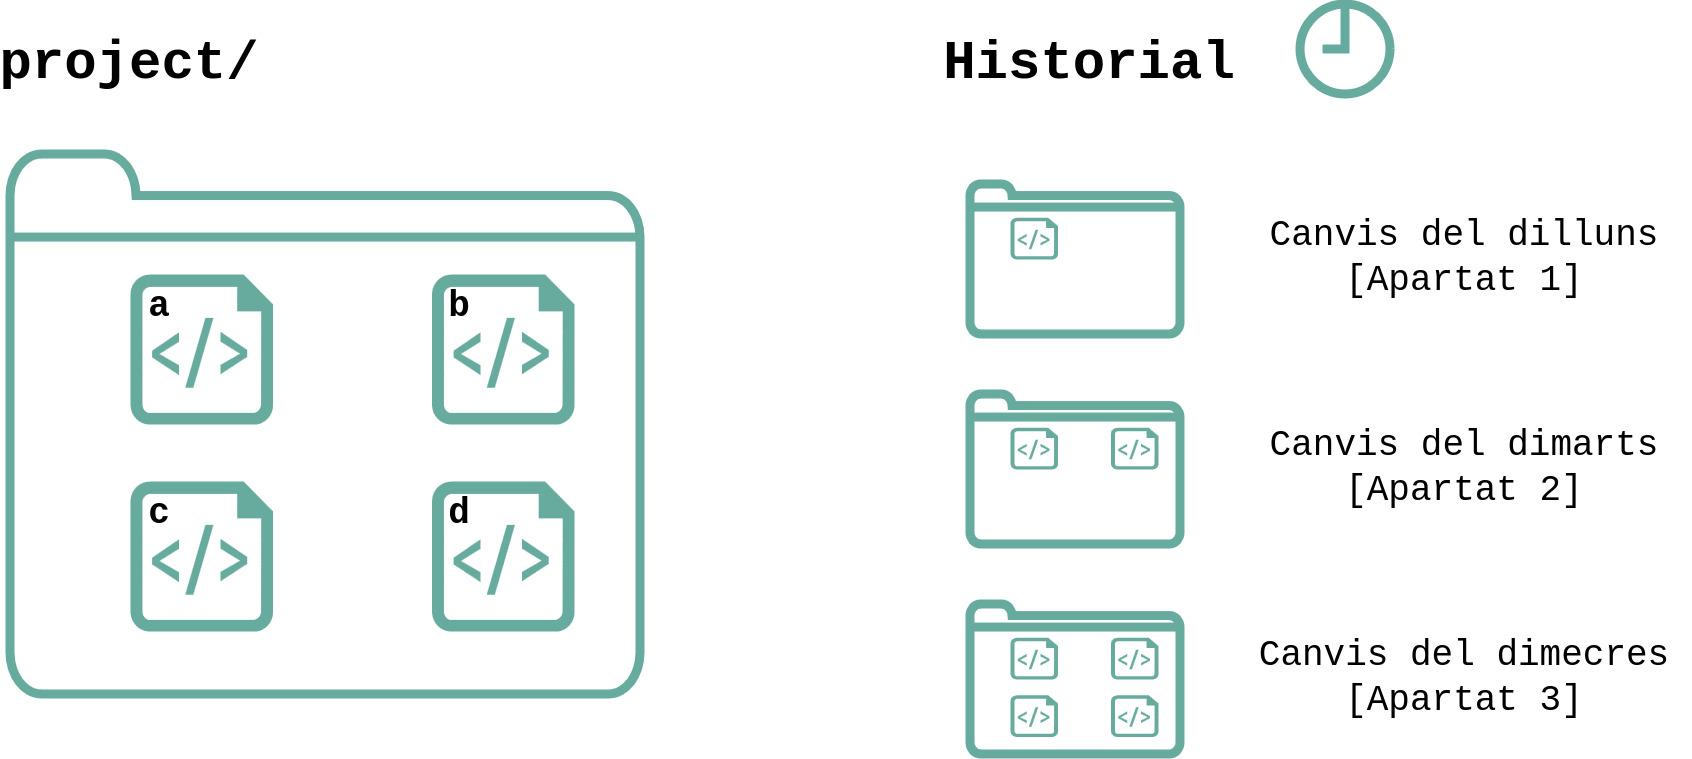
\includegraphics[scale=0.18]{images/perque}}\label{fig:figure}
        \end{figure}
    \end{frame}
    \begin{frame}
        \frametitle{Why Git?}
        \begin{itemize}
            \item \texttt{git init}: Create a new repository in the current directory
            \item \texttt{git add <file>}: Add a file to the staging area (. adds the whole directory)
            \item \texttt{git commit -m "message"}: Commit the changes in the staging area
        \end{itemize}
    \end{frame}
    \begin{frame}
        \frametitle{Why Git?}
        \begin{figure}[H]
            \centering
            \noindent
            \makebox[\textwidth]{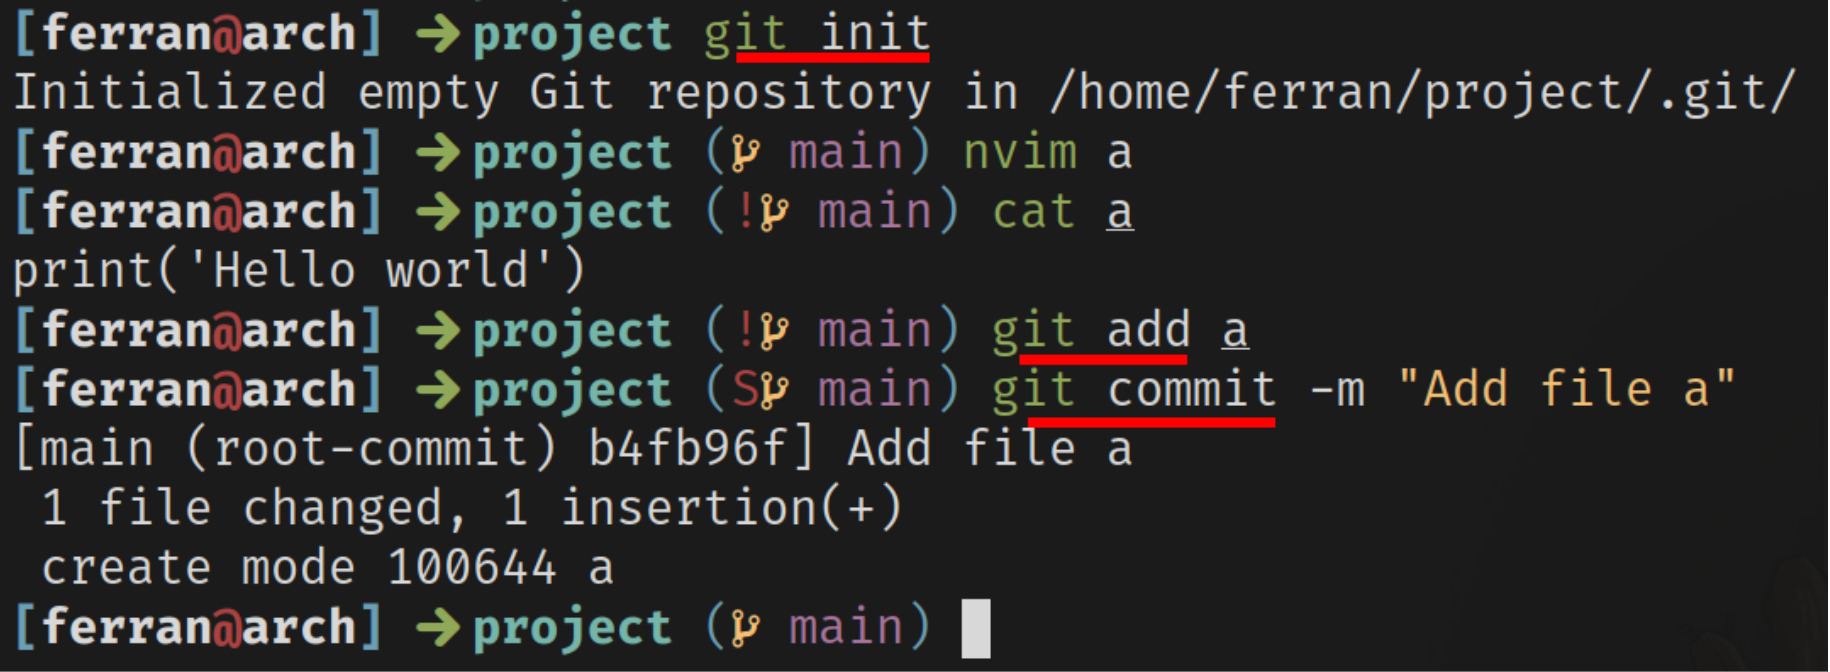
\includegraphics[scale=0.15]{images/com1}}
        \end{figure}
    \end{frame}


    \section{Basics}\label{sec:basics}

    \subsection{Basic commands}\label{subsec:basic-commands}
    \begin{frame}
        \frametitle{Basics}
        \begin{figure}[H]
            \centering
            \noindent
            \makebox[\textwidth]{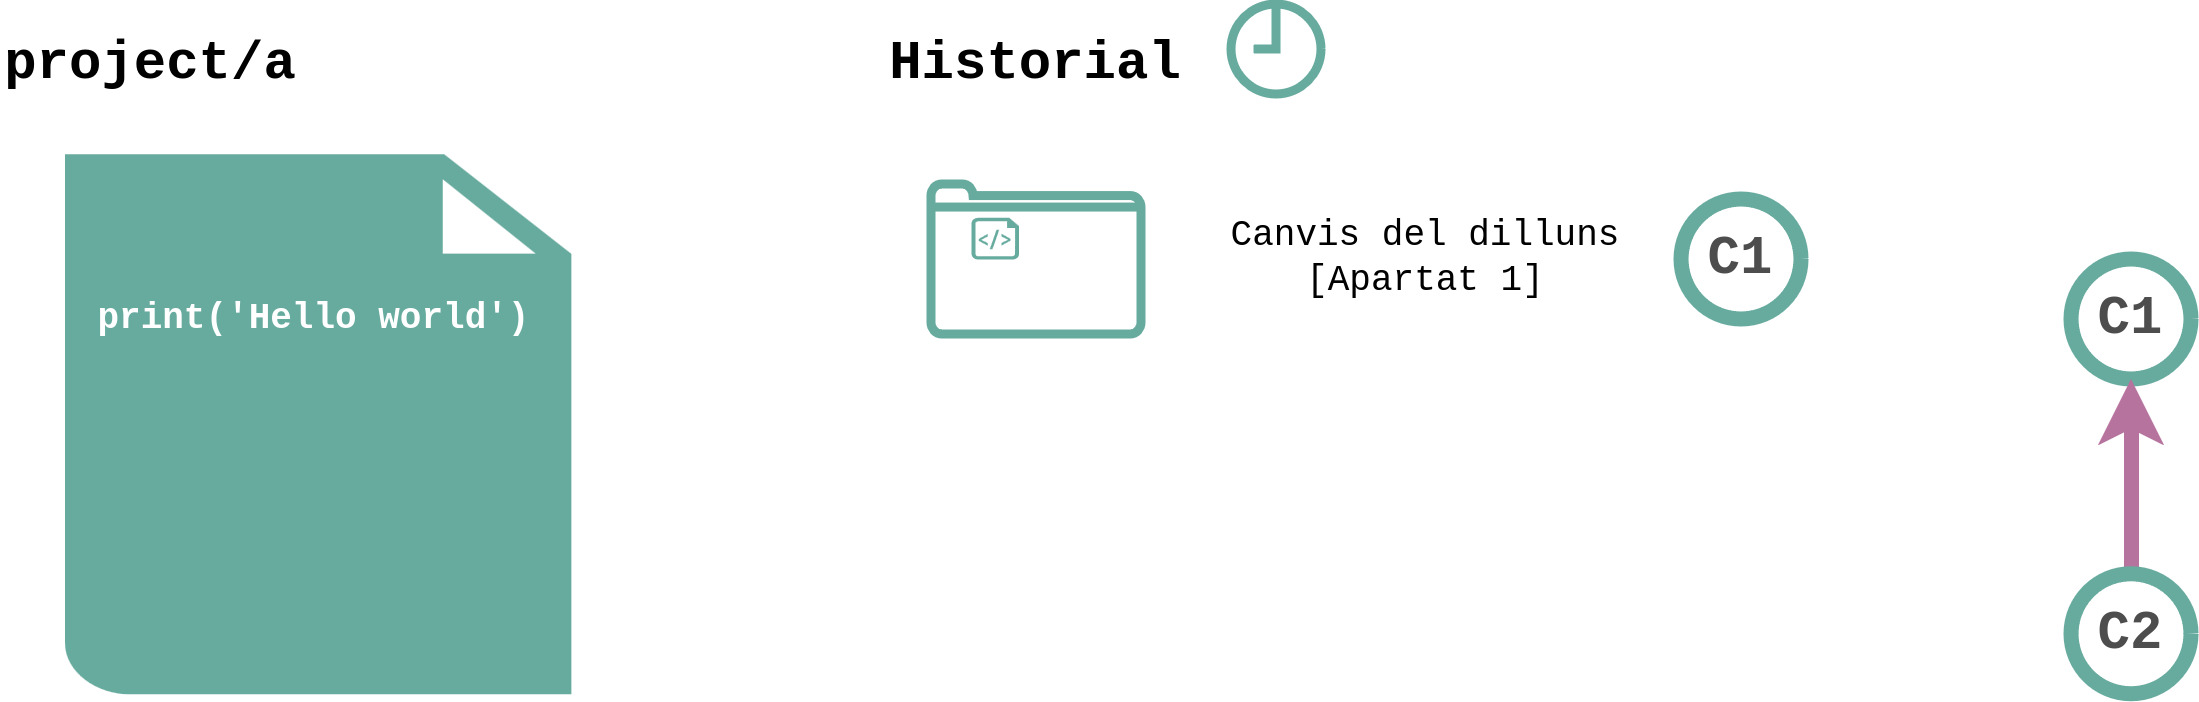
\includegraphics[scale=0.12]{images/basics}}\label{fig:figure2}
        \end{figure}
    \end{frame}
    \begin{frame}
        \begin{itemize}
            \item \texttt{git status}: Check the status of the repository
            \item \texttt{git diff}: Show the changes between the working directory and the staging area
        \end{itemize}
    \end{frame}

    \subsection{Staging}\label{subsec:staging}
    \begin{frame}
        \frametitle{Staging area, git diff and status}
        \begin{figure}[H]
            \centering
            \noindent
            \makebox[\textwidth]{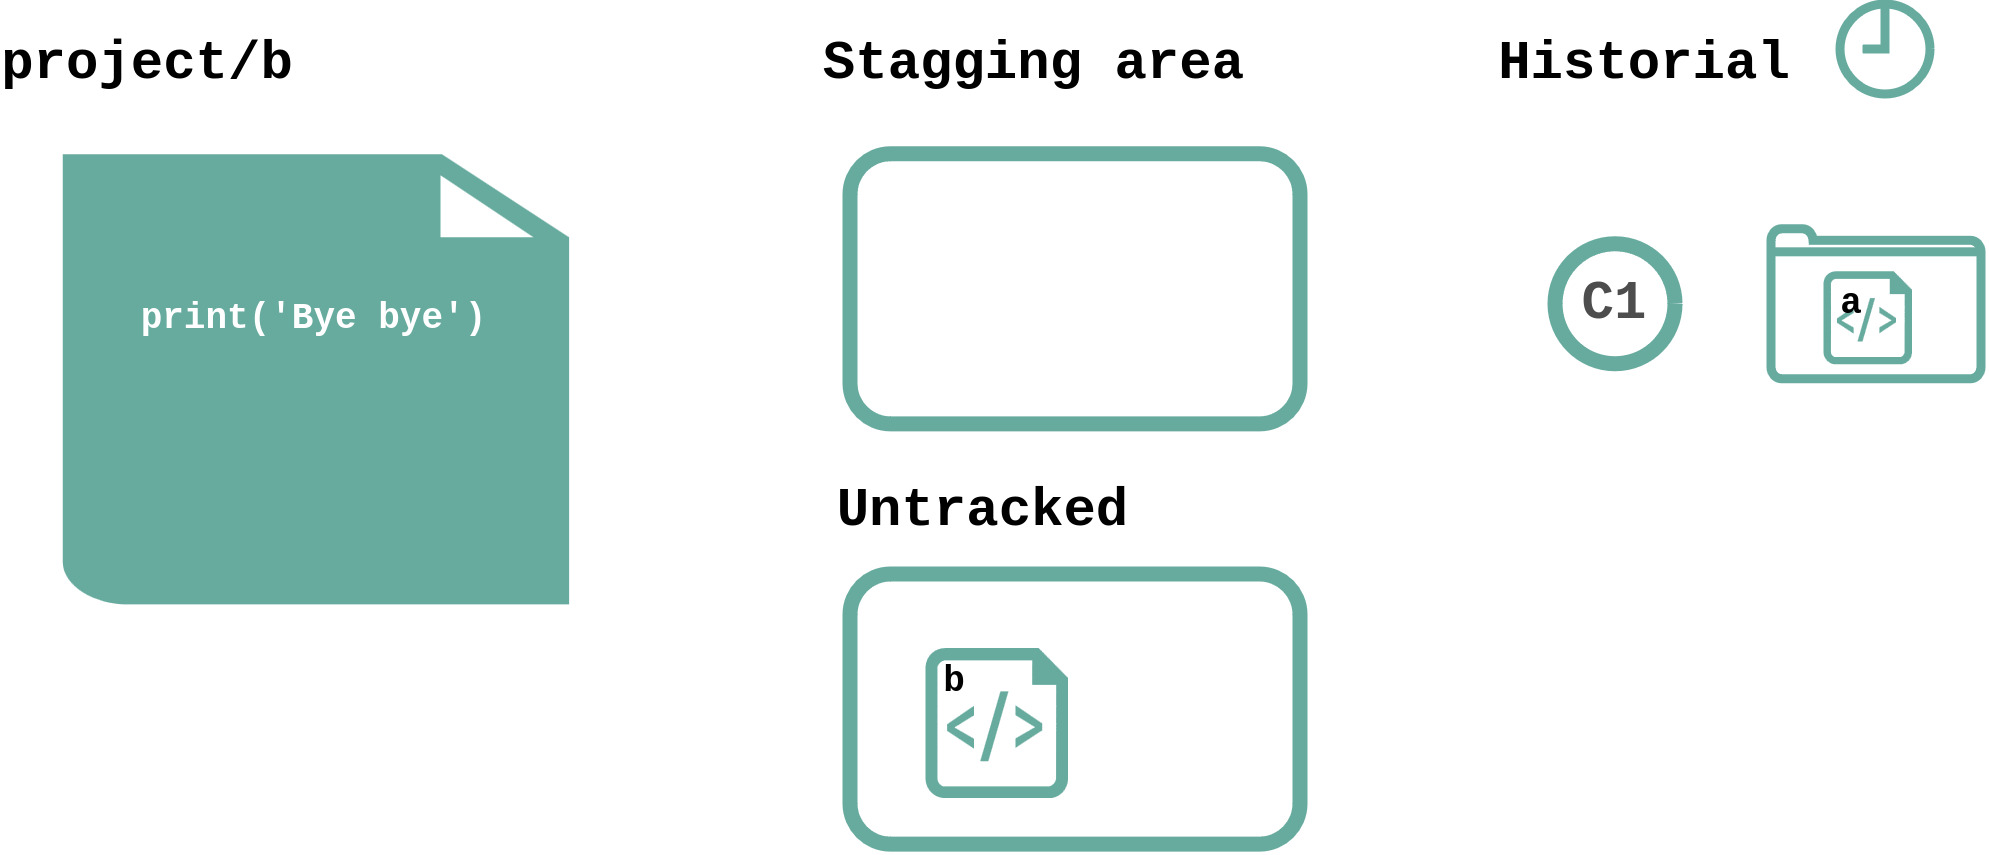
\includegraphics[scale=0.15]{images/staging}}\label{fig:figure3}
        \end{figure}
    \end{frame}
    \begin{frame}
        \frametitle{Staging area, git diff and status}
        \begin{figure}[H]
            \centering
            \noindent
            \makebox[\textwidth]{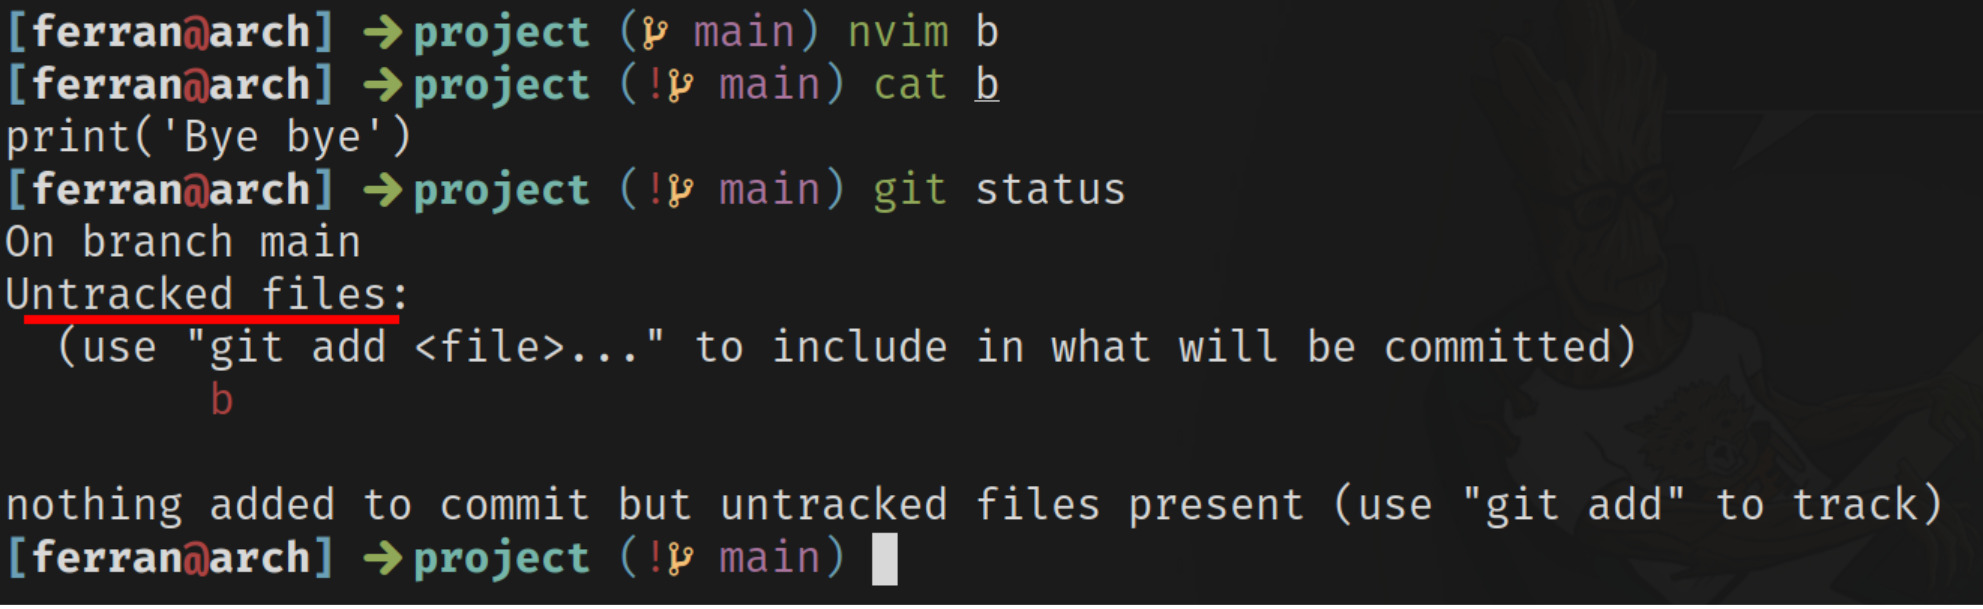
\includegraphics[scale=0.15]{images/com2}}
        \end{figure}
    \end{frame}
    \begin{frame}
        \frametitle{Staging area, git diff and status}
        \begin{figure}[H]
            \centering
            \noindent
            \makebox[\textwidth]{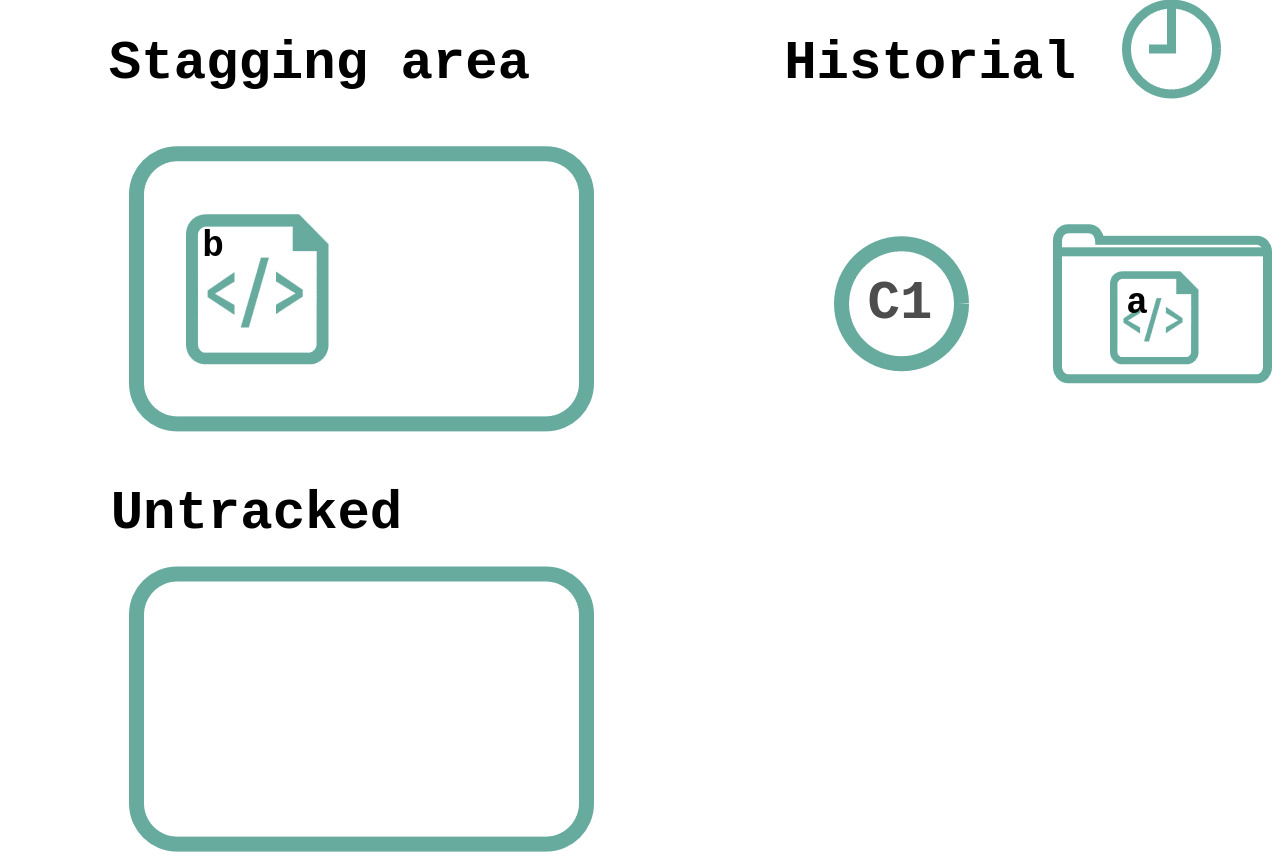
\includegraphics[scale=0.15]{images/staging-2}}\label{fig:figure4}
        \end{figure}
    \end{frame}
    \begin{frame}
        \frametitle{Staging area, git diff and status}
        \begin{figure}[H]
            \centering
            \noindent
            \makebox[\textwidth]{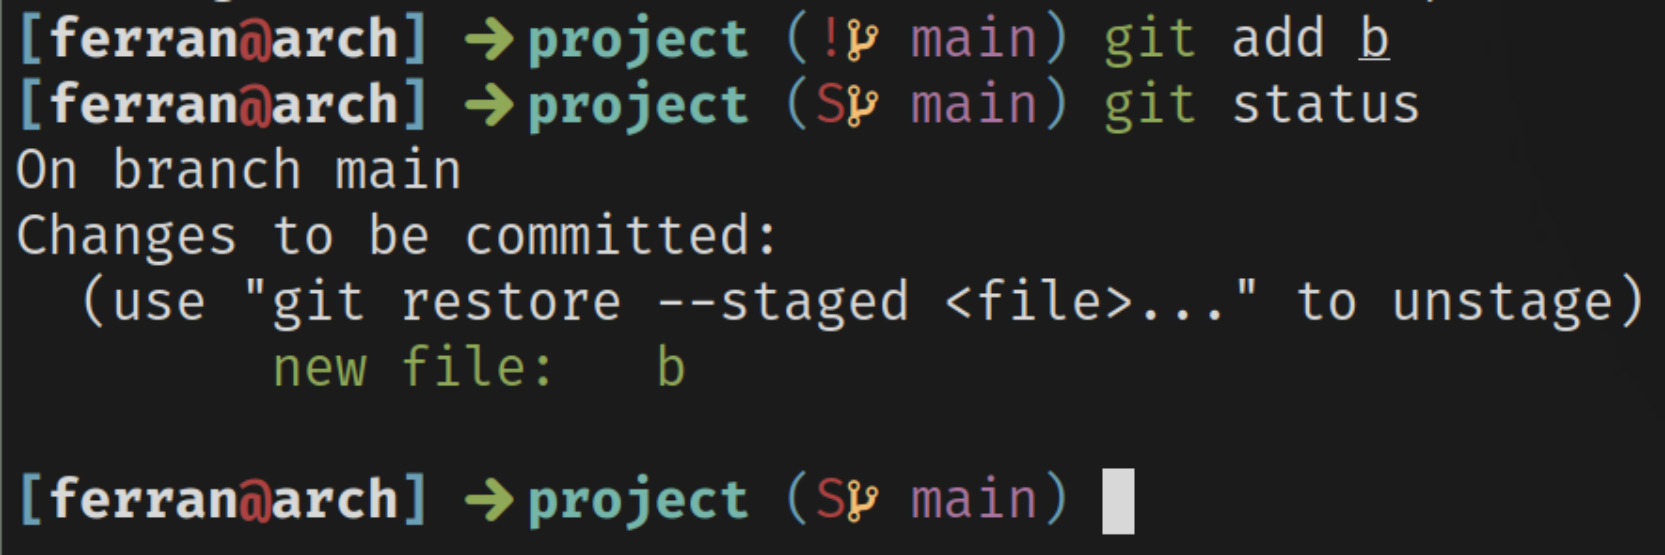
\includegraphics[scale=0.15]{images/com3}}
        \end{figure}
    \end{frame}
    \begin{frame}
        \frametitle{Staging area, git diff and status}
        \begin{figure}[H]
            \centering
            \noindent
            \makebox[\textwidth]{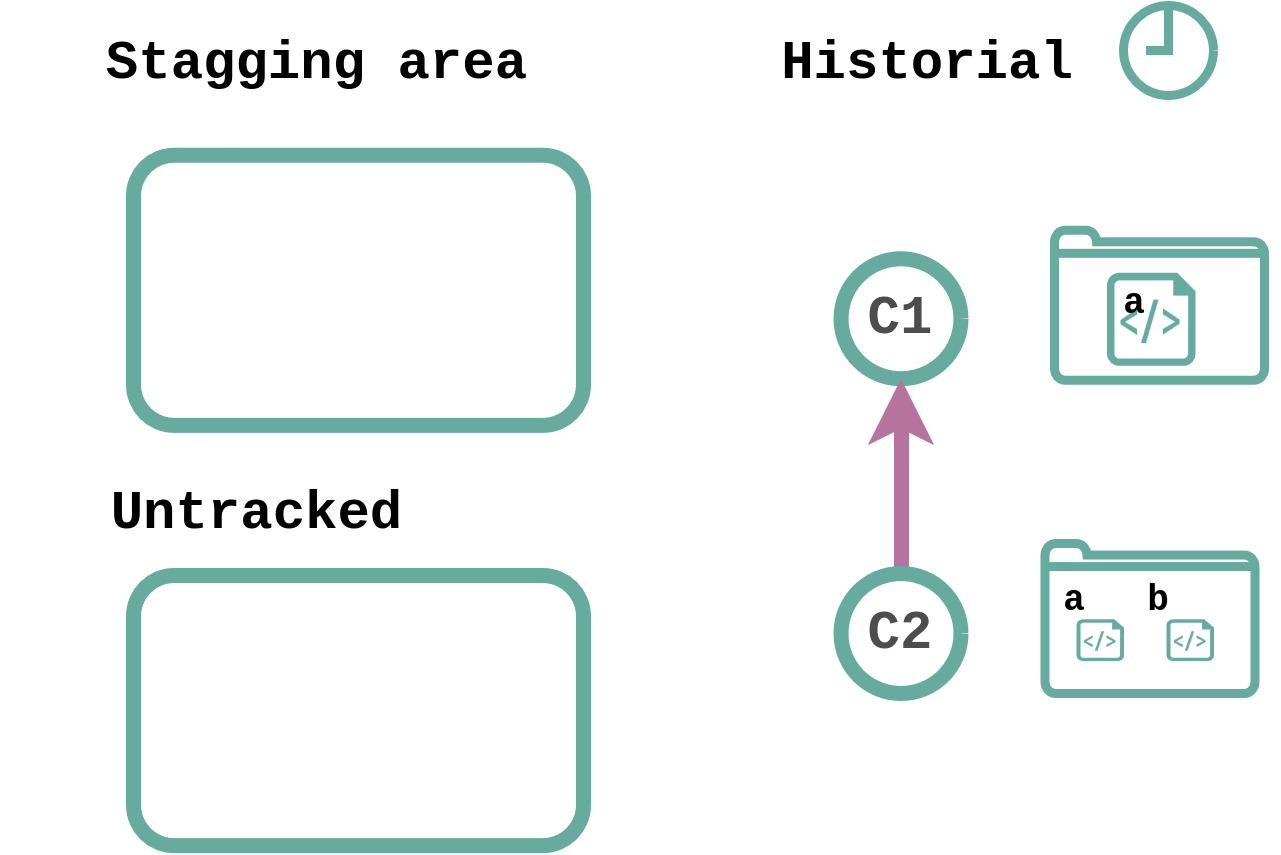
\includegraphics[scale=0.15]{images/staging-3}}\label{fig:figure5}
        \end{figure}
    \end{frame}
    \begin{frame}
        \frametitle{Staging area, git diff and status}
        \begin{figure}[H]
            \centering
            \noindent
            \makebox[\textwidth]{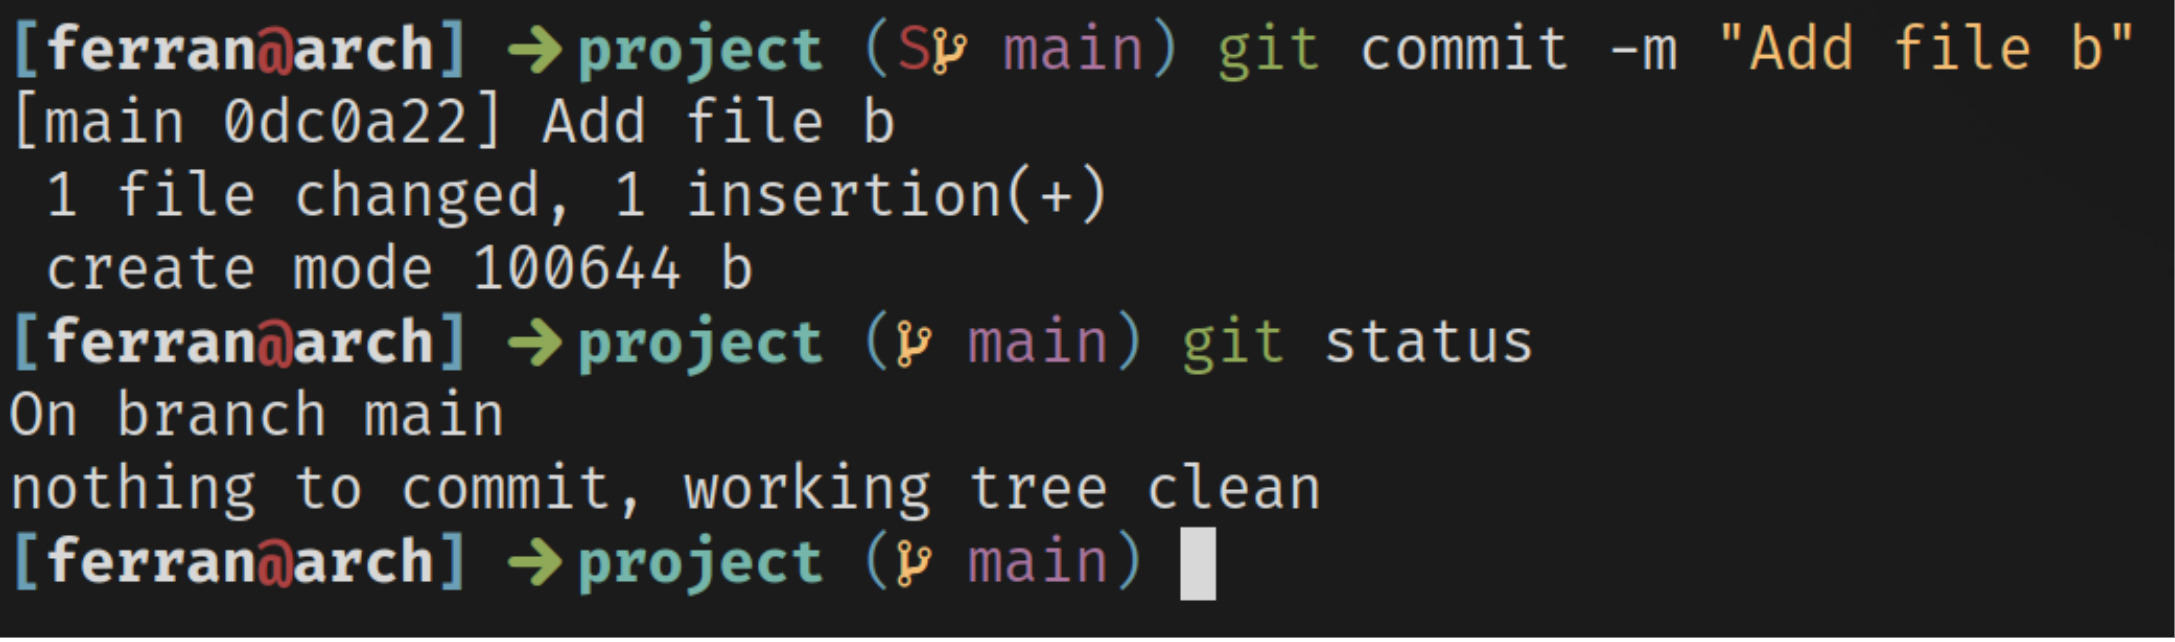
\includegraphics[scale=0.15]{images/com4}}
        \end{figure}
    \end{frame}
    \begin{frame}
        \frametitle{Staging area, git diff and status}
        \begin{figure}[H]
            \centering
            \noindent
            \makebox[\textwidth]{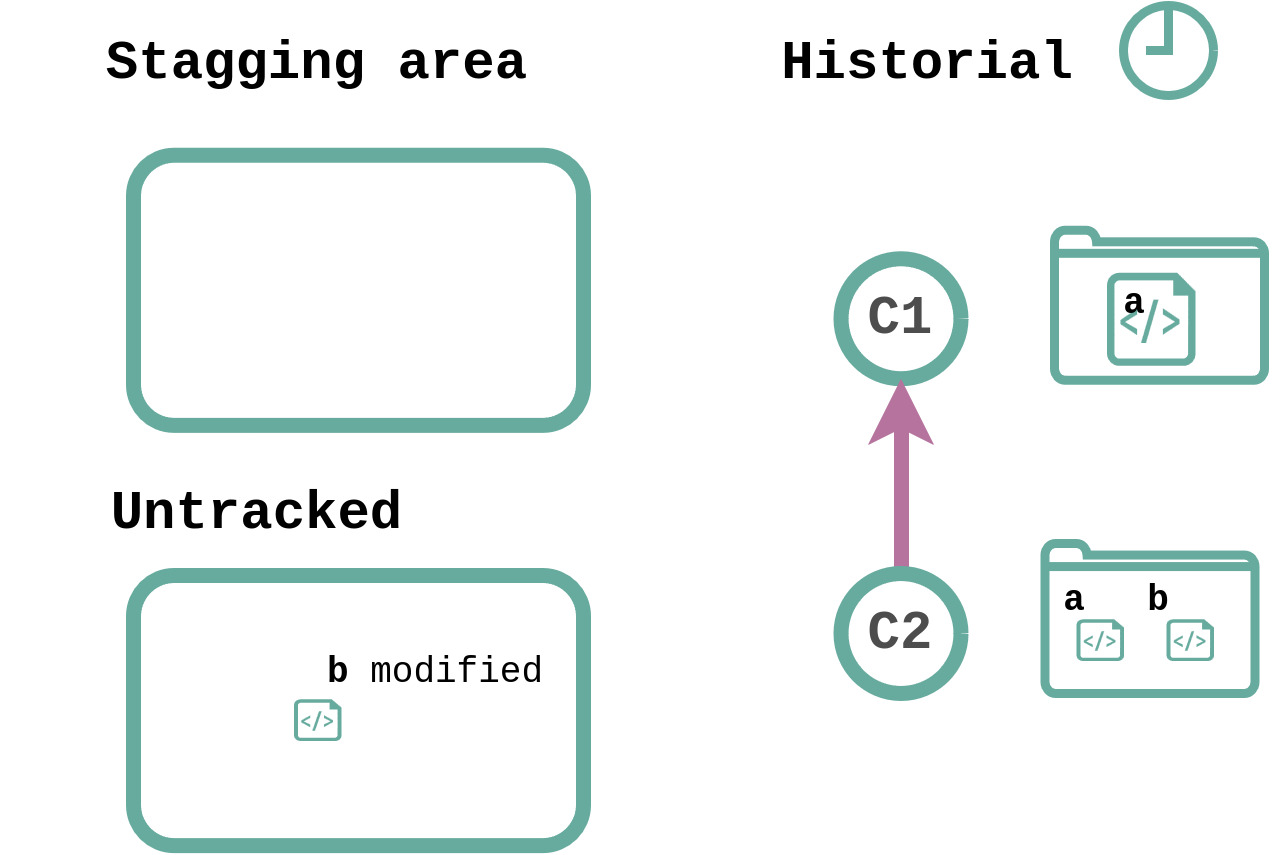
\includegraphics[scale=0.15]{images/staging-4}}\label{fig:figure6}
        \end{figure}
    \end{frame}
    \begin{frame}
        \frametitle{Staging area, git diff and status}
        \begin{figure}[H]
            \centering
            \noindent
            \makebox[\textwidth]{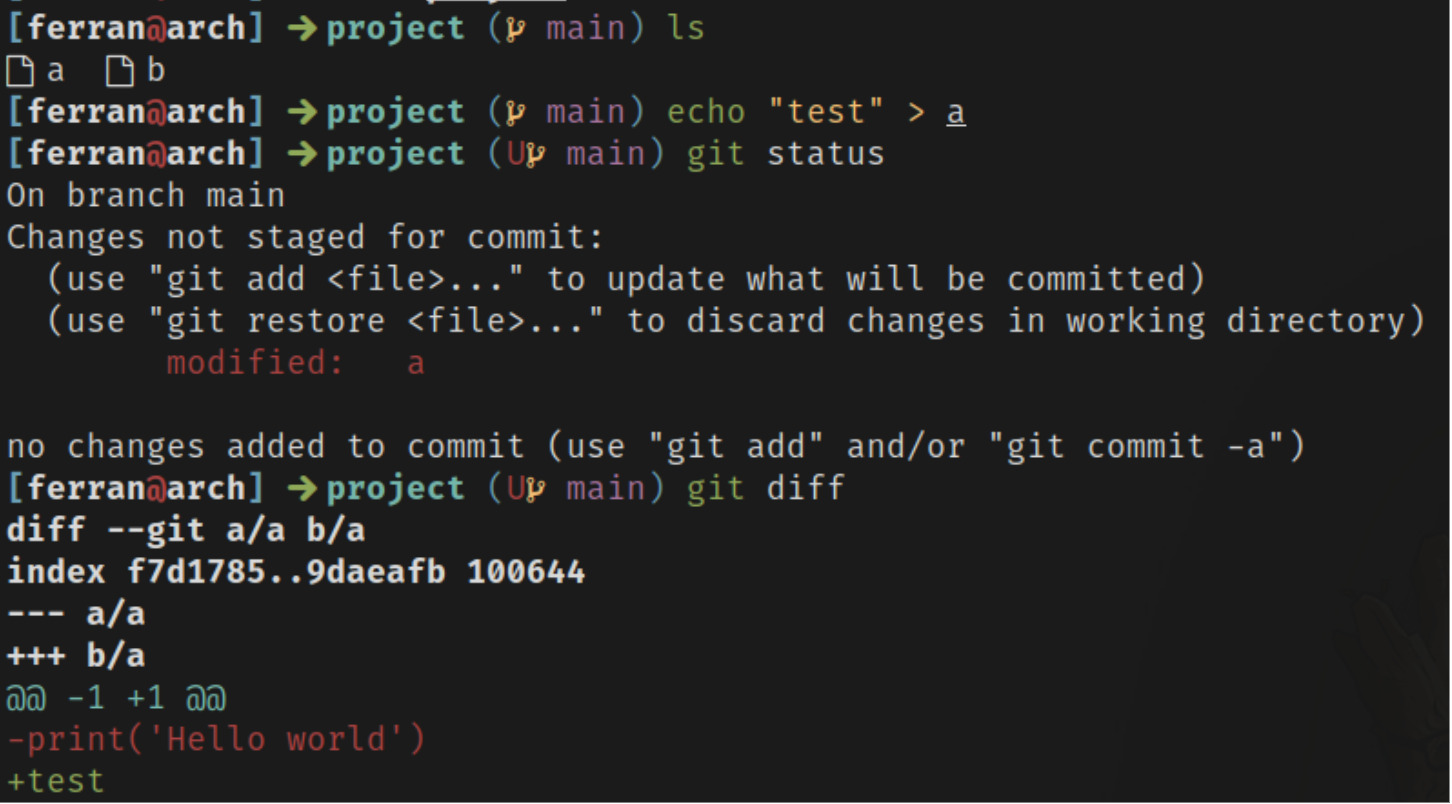
\includegraphics[scale=0.15]{images/com5}}
        \end{figure}
    \end{frame}
    \begin{frame}
        \frametitle{Staging area, git diff and status}
        \begin{figure}[H]
            \centering
            \noindent
            \makebox[\textwidth]{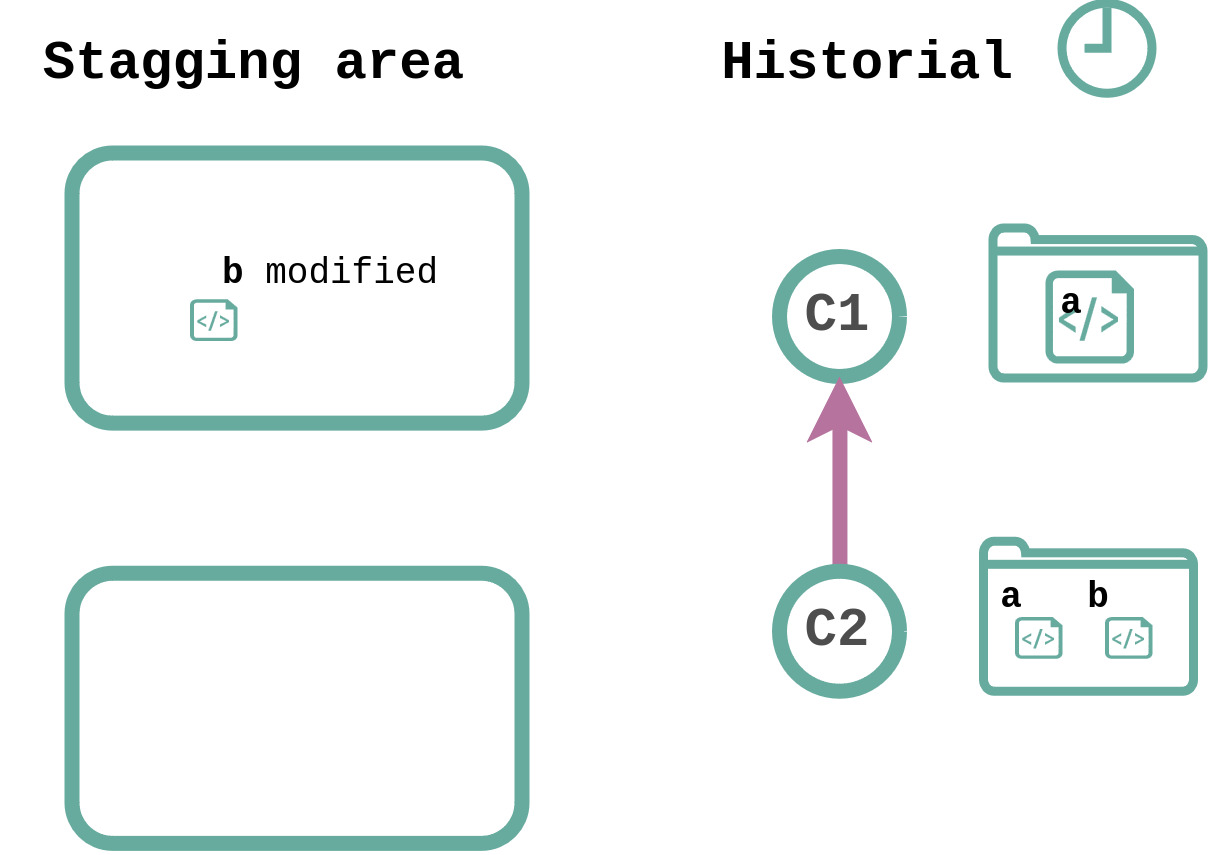
\includegraphics[scale=0.15]{images/staging-5}}\label{fig:figure7}
        \end{figure}
    \end{frame}
    \begin{frame}
        \frametitle{Staging area, git diff and status}
        \begin{figure}[H]
            \centering
            \noindent
            \makebox[\textwidth]{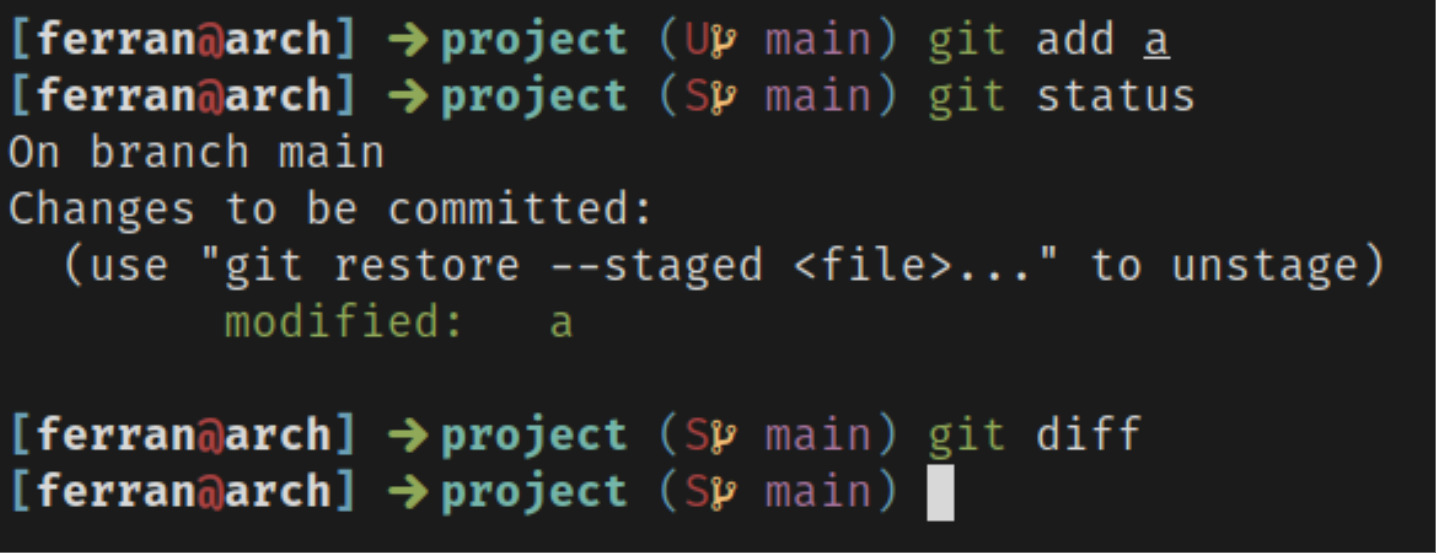
\includegraphics[scale=0.15]{images/com6}}
        \end{figure}
    \end{frame}

    \subsection{Remotes}\label{subsec:remotes}
    \begin{frame}
        \frametitle{Working with remotes}
        \begin{figure}[H]
            \centering
            \noindent
            \makebox[\textwidth]{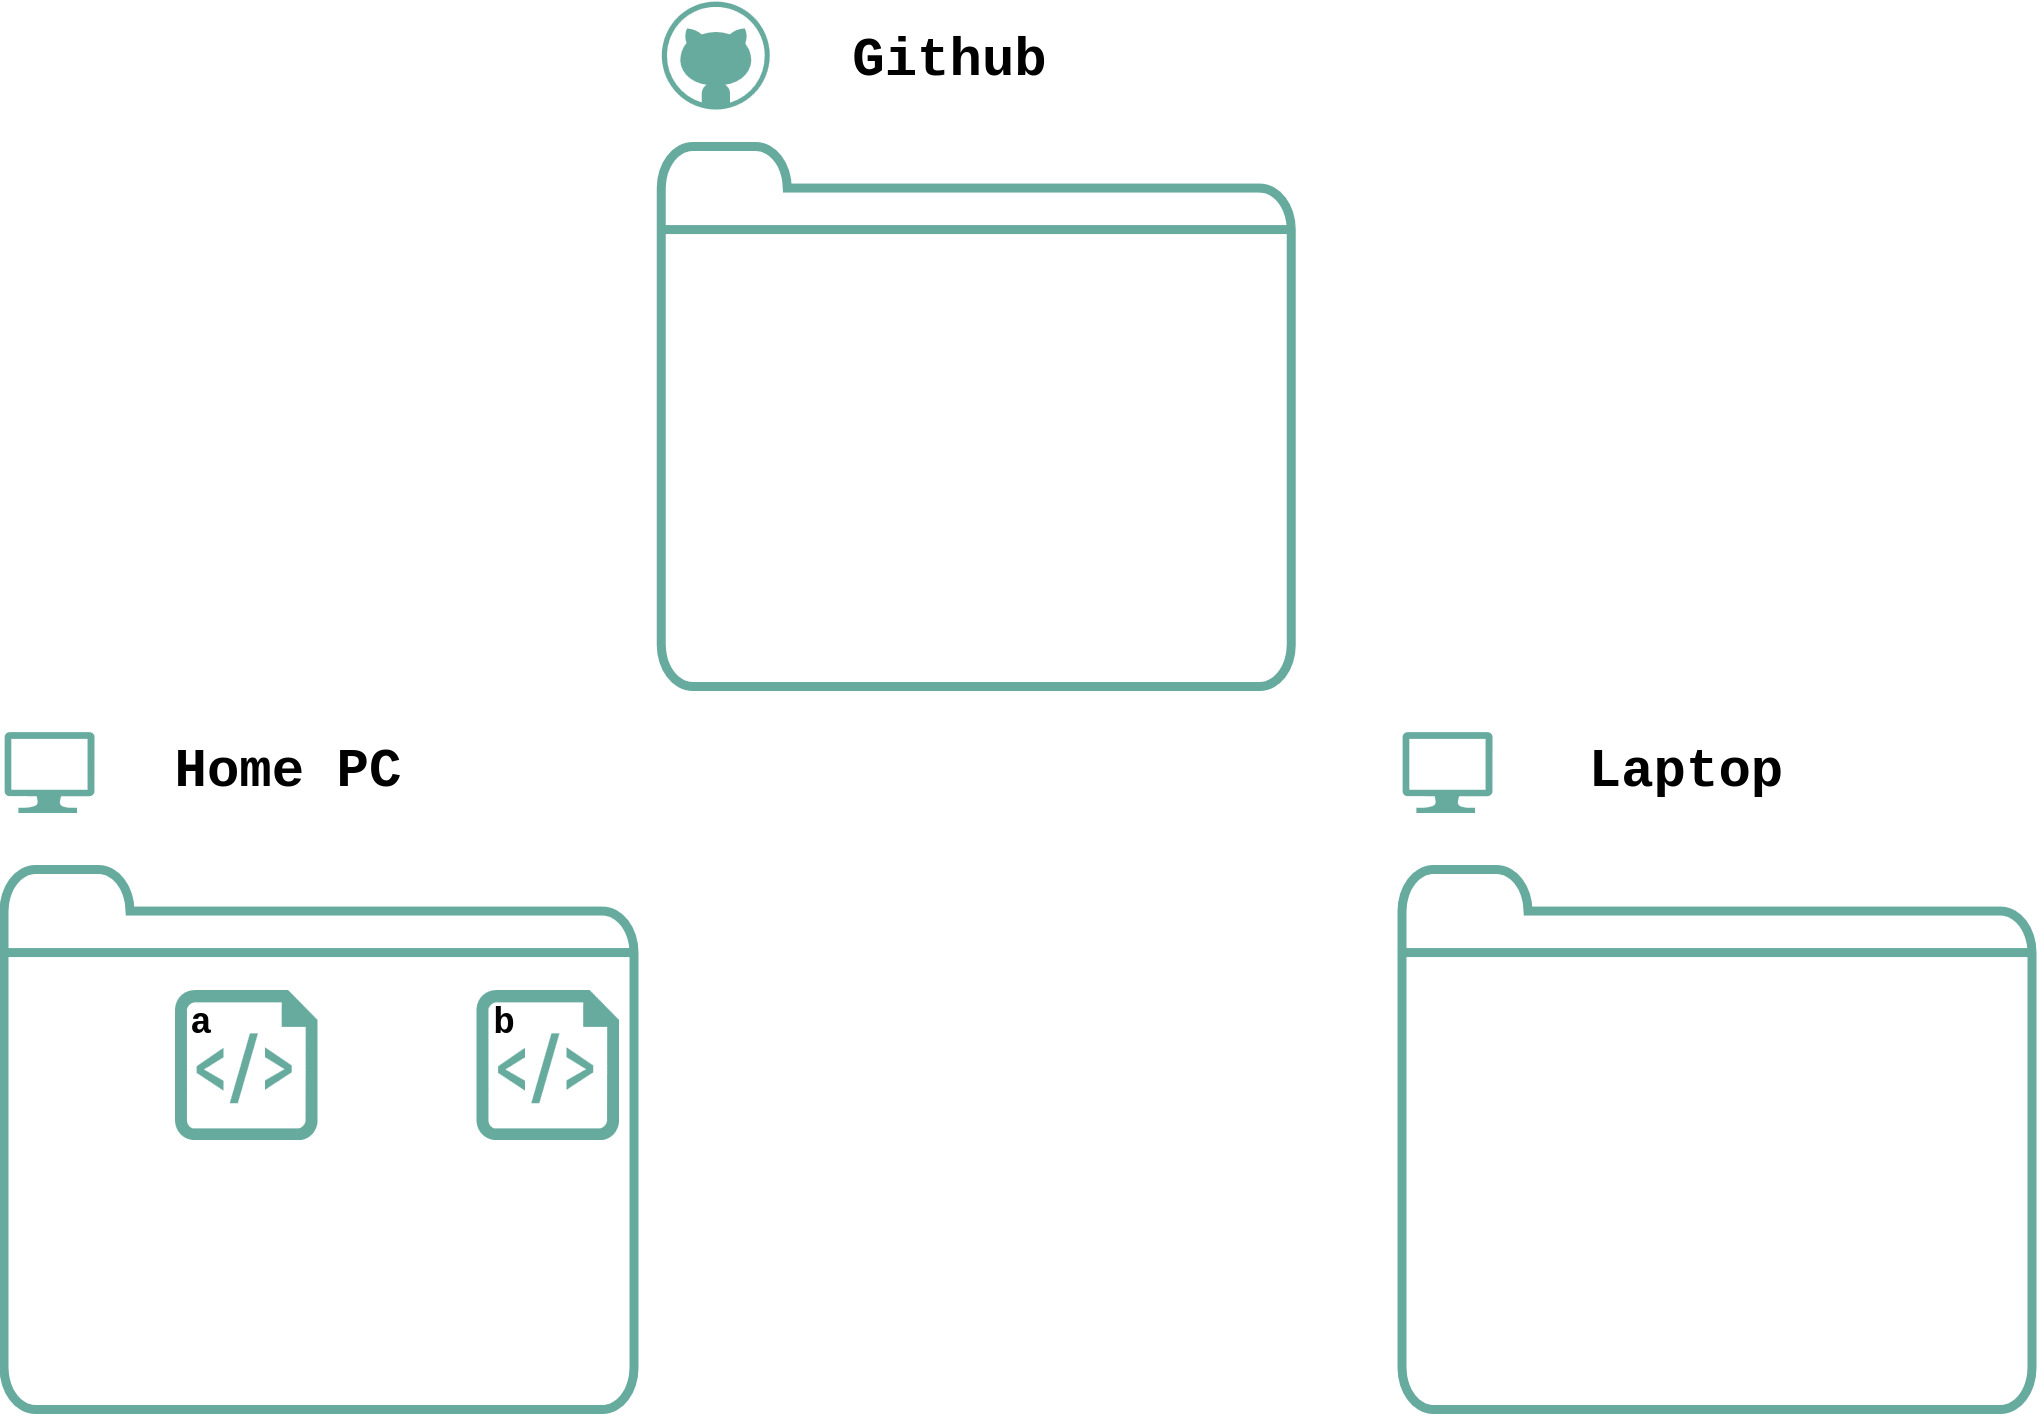
\includegraphics[scale=0.12]{images/remote}}
        \end{figure}
    \end{frame}
    \begin{frame}
        \frametitle{Working with remotes}
        \begin{itemize}
            \item \texttt{git remote add <name> <url>}: Add a remote repository
            \item \texttt{git branch -M main}: Rename the current branch to main
            \item \texttt{git push -u <remote> <branch>}: Push the current branch to the remote repository
            \item \texttt{git pull <remote> <branch>}: Pull the changes from the remote repository
        \end{itemize}
    \end{frame}
    \begin{frame}
        \frametitle{Working with remotes}
        \begin{figure}[H]
            \centering
            \noindent
            \makebox[\textwidth]{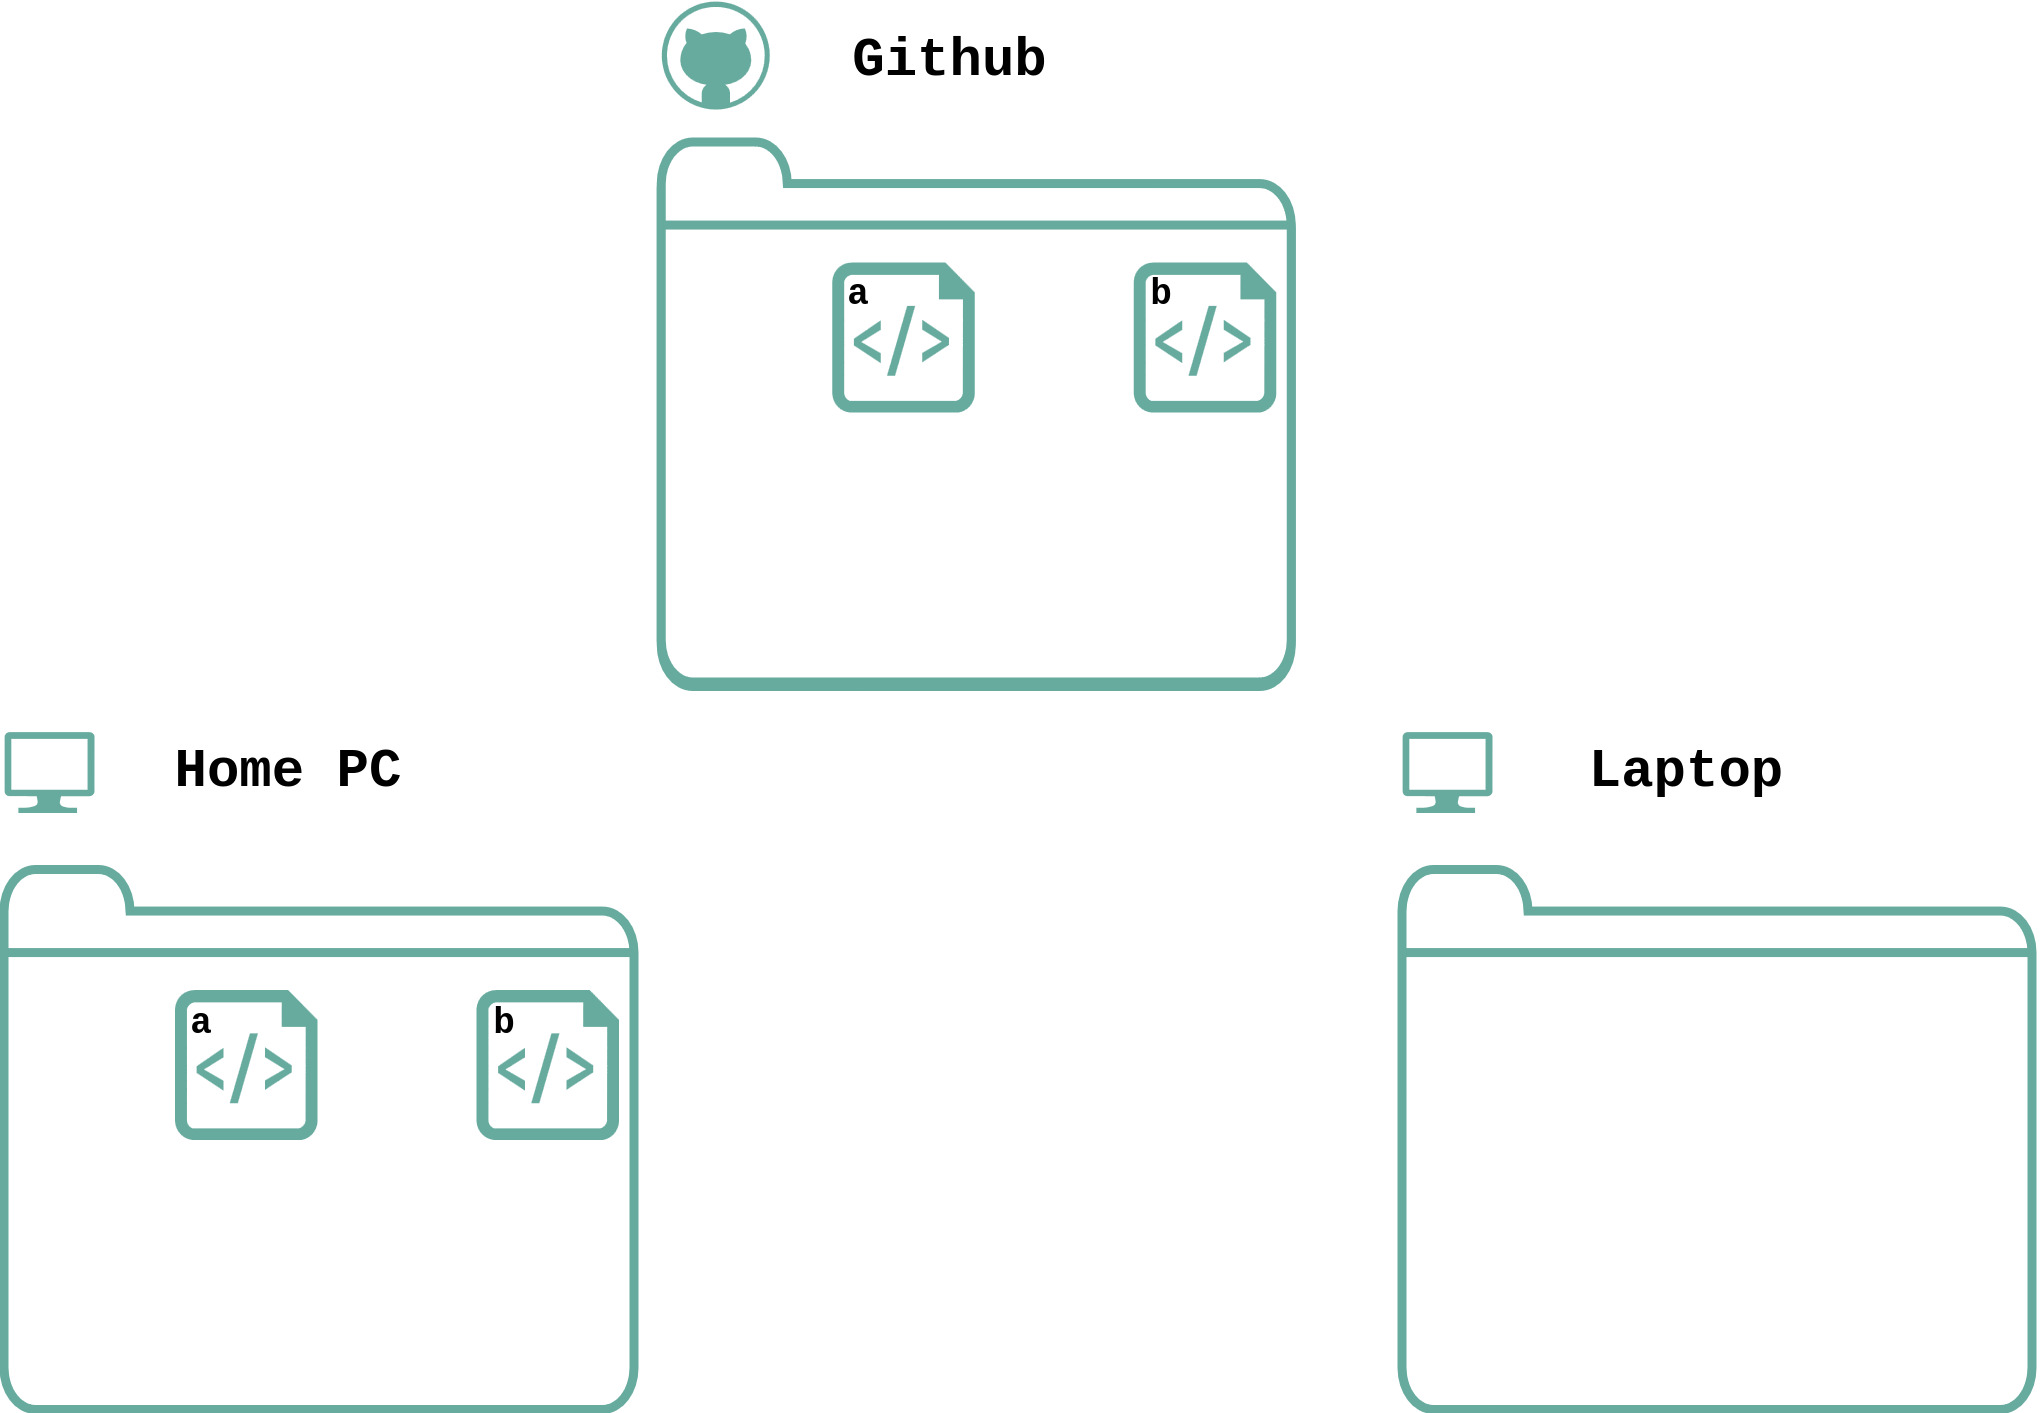
\includegraphics[scale=0.12]{images/remote-2}}
        \end{figure}
    \end{frame}
    \begin{frame}
        \frametitle{Working with remotes}
        \begin{figure}[H]
            \centering
            \noindent
            \makebox[\textwidth]{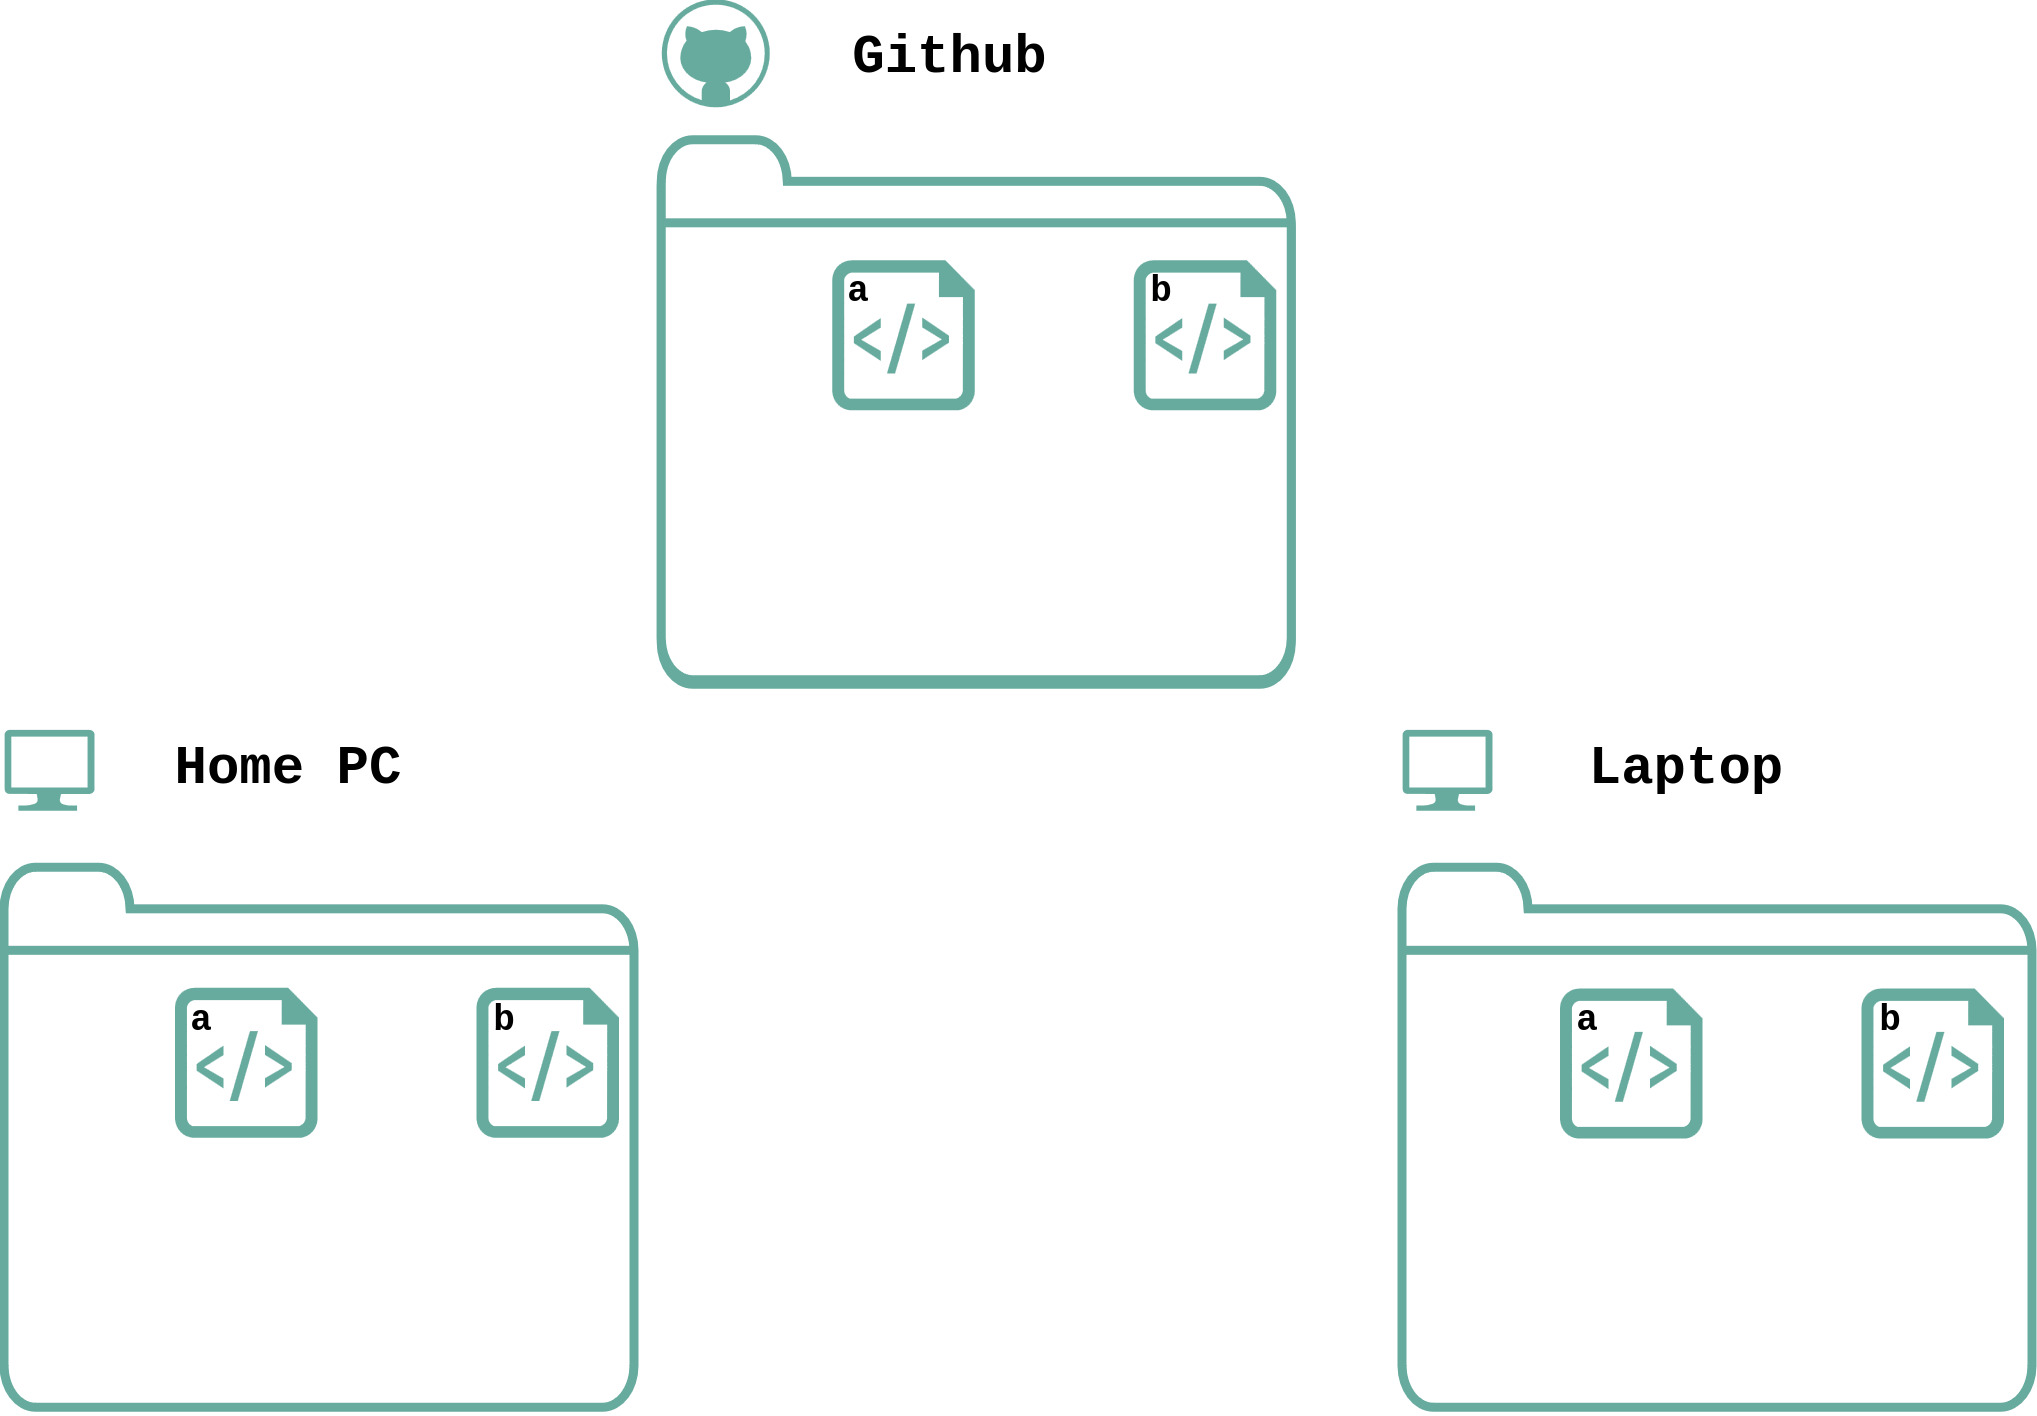
\includegraphics[scale=0.12]{images/remote-3}}
        \end{figure}
    \end{frame}
    \begin{frame}
        \frametitle{Working with remotes}
        \begin{figure}[H]
            \centering
            \noindent
            \makebox[\textwidth]{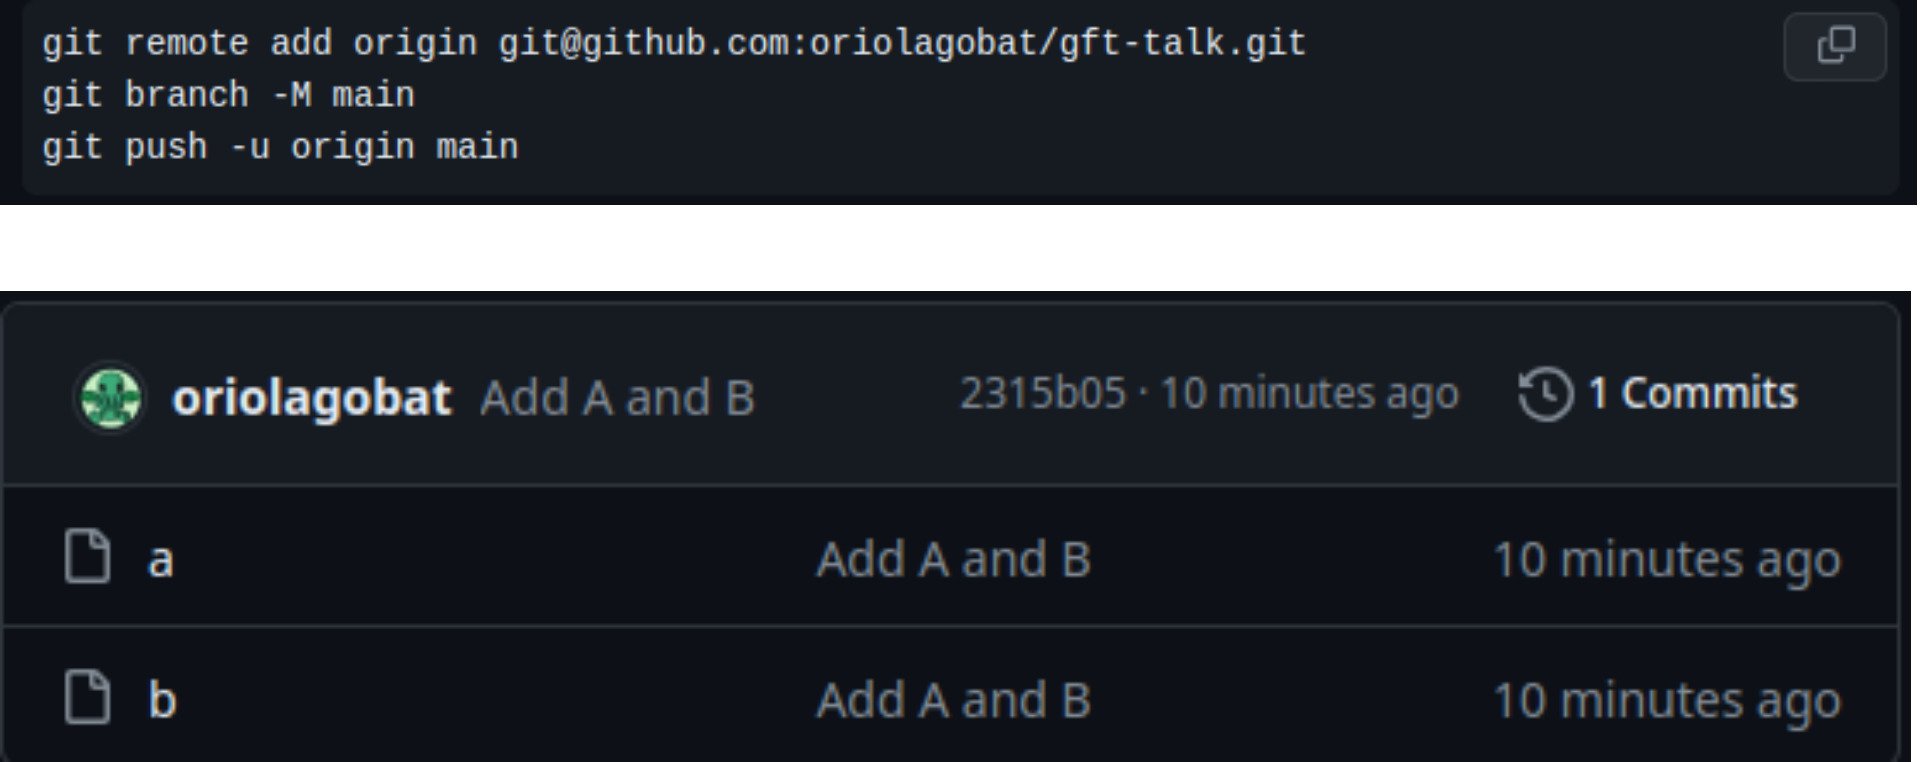
\includegraphics[scale=0.15]{images/com10}}
        \end{figure}
    \end{frame}
    \begin{frame}
        \frametitle{Working with remotes}
        \begin{figure}[H]
            \centering
            \noindent
            \makebox[\textwidth]{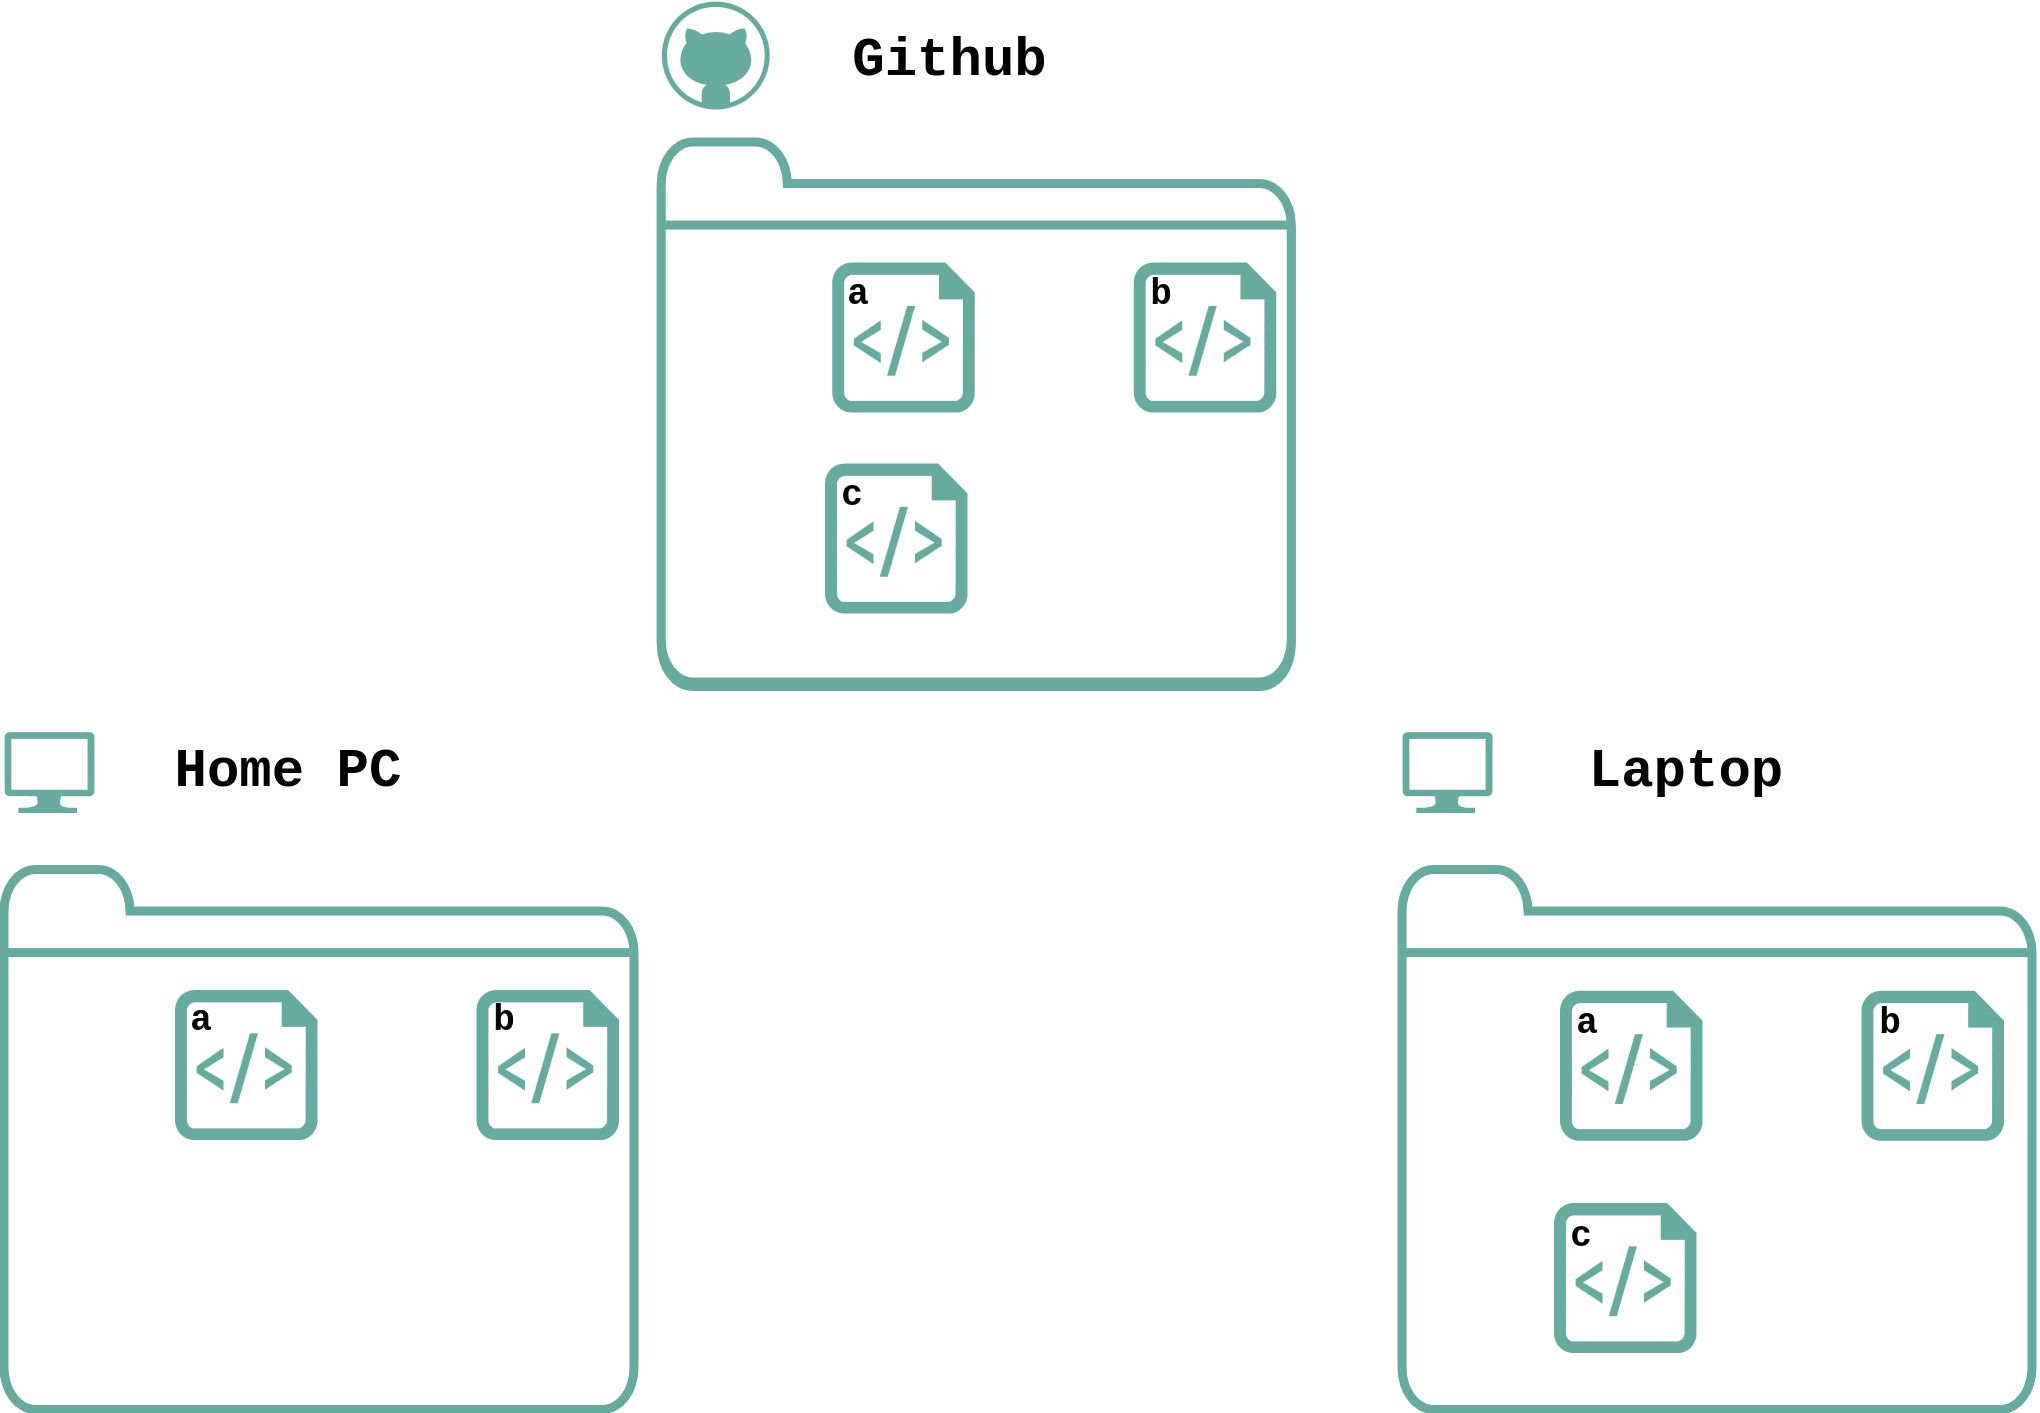
\includegraphics[scale=0.12]{images/remote-4}}
        \end{figure}
    \end{frame}
    \begin{frame}
        \frametitle{Working with remotes}
        \begin{figure}[H]
            \centering
            \noindent
            \makebox[\textwidth]{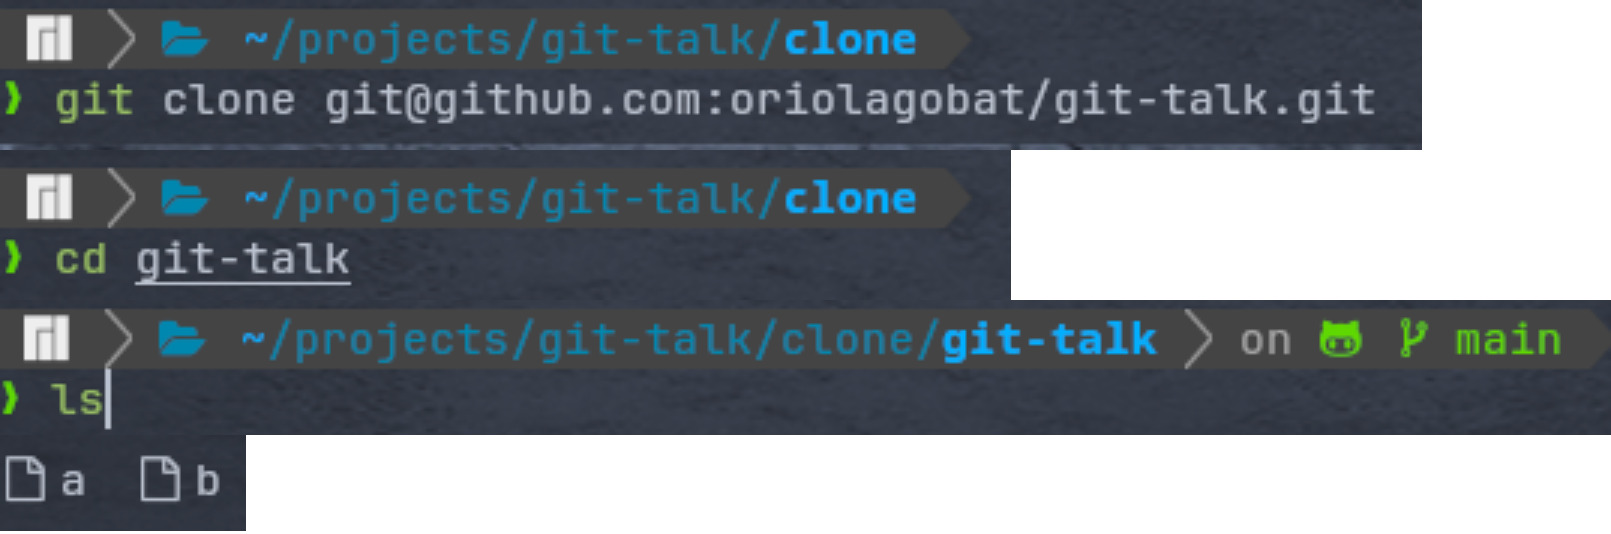
\includegraphics[scale=0.15]{images/com11}}
        \end{figure}
    \end{frame}
    \begin{frame}
        \frametitle{Working with remotes}
        \begin{figure}[H]
            \centering
            \noindent
            \makebox[\textwidth]{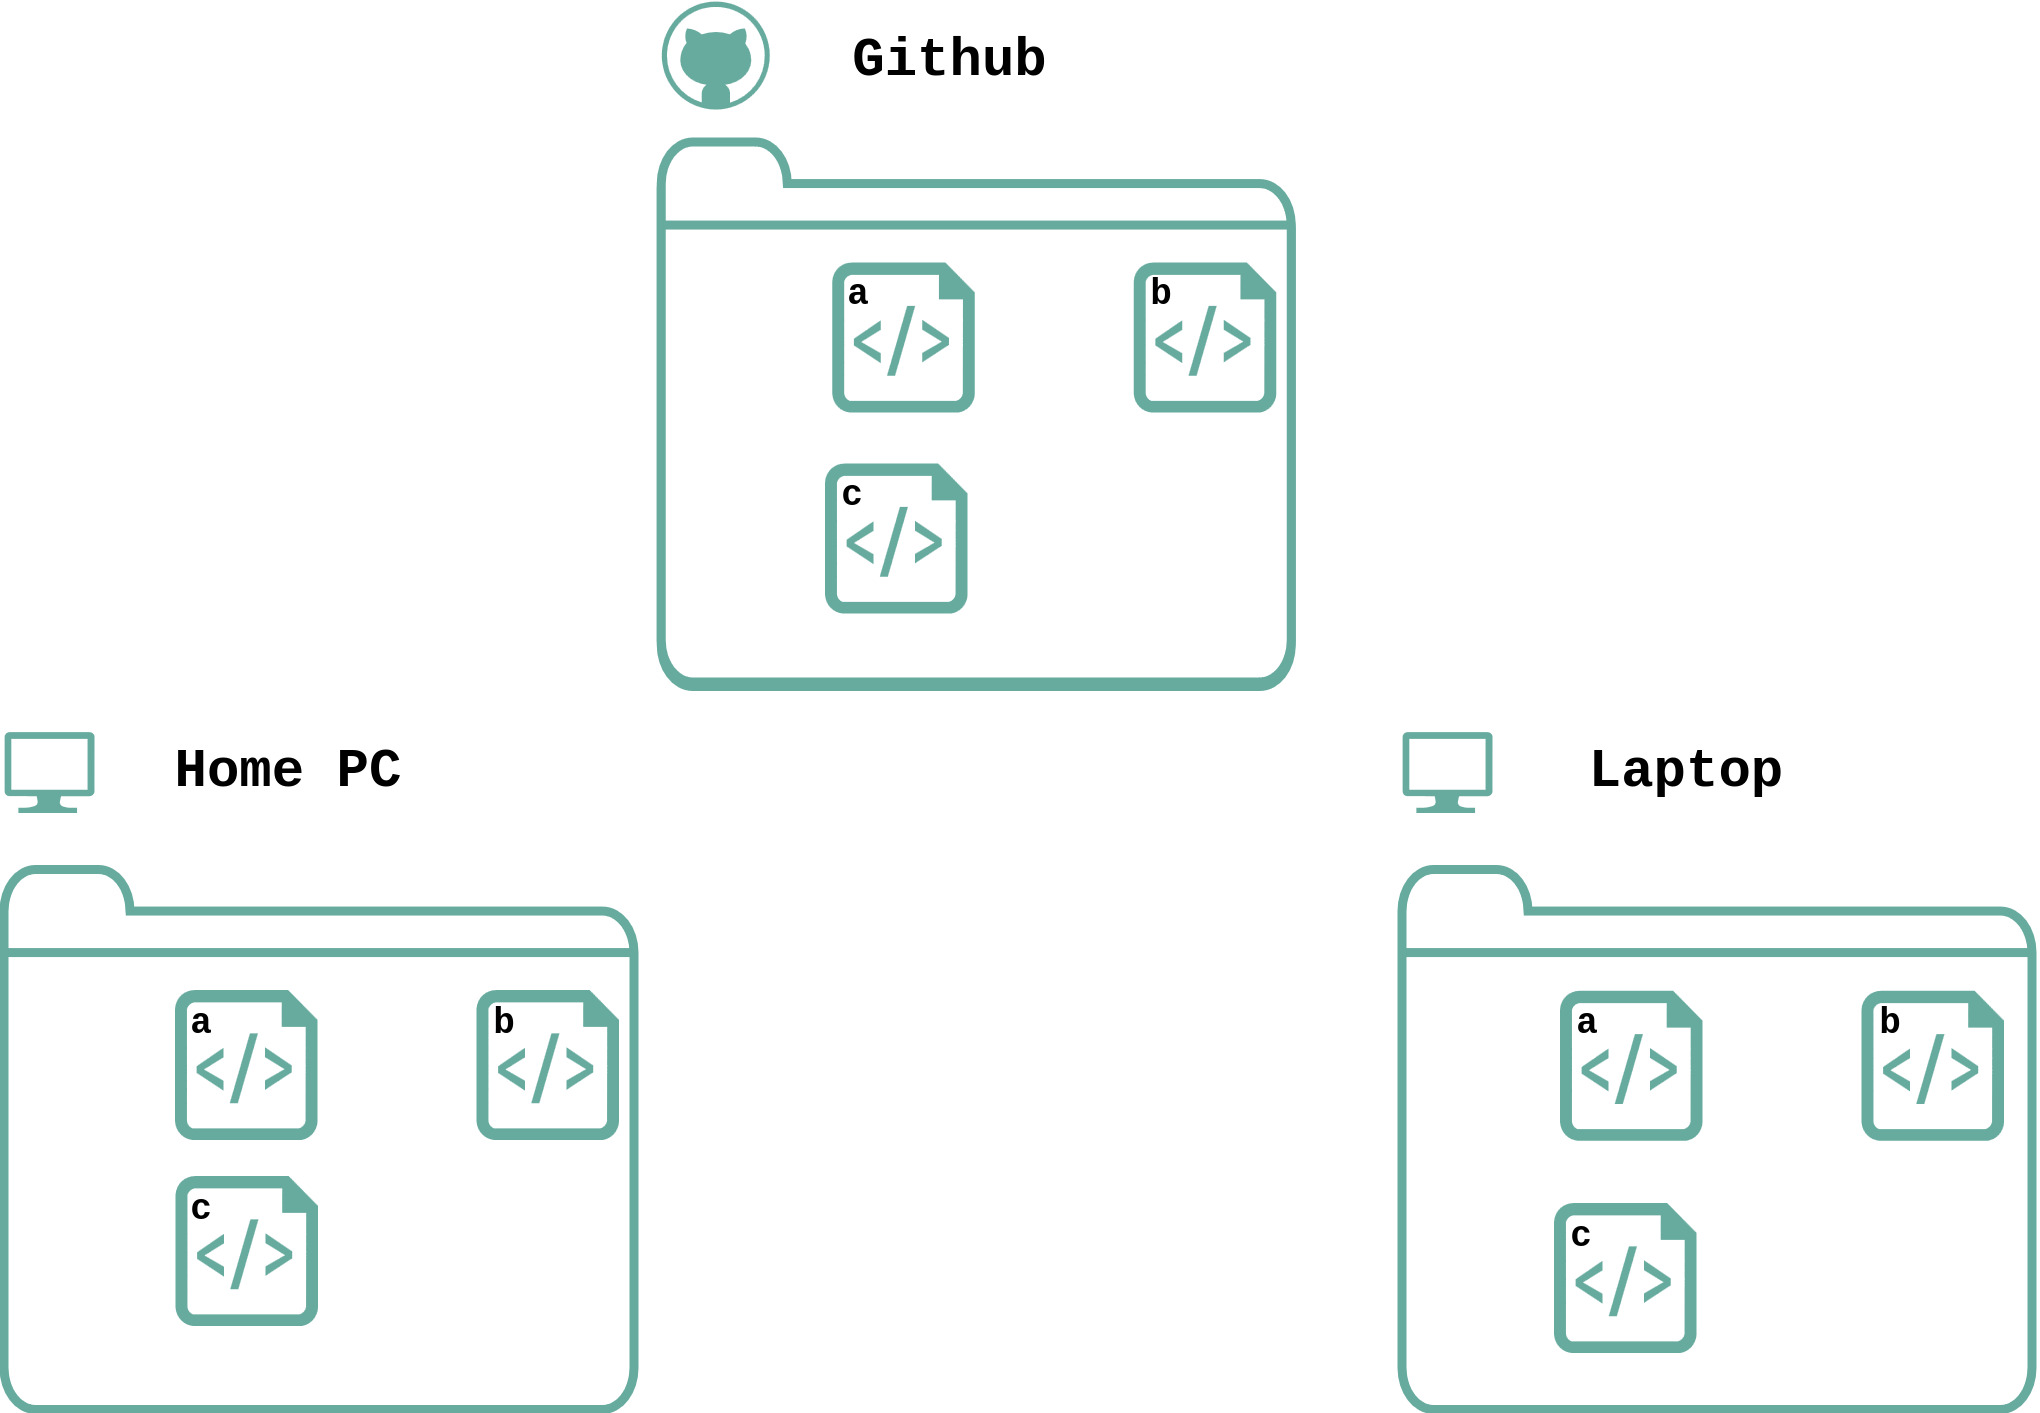
\includegraphics[scale=0.12]{images/remote-5}}
        \end{figure}
    \end{frame}
    \begin{frame}
        \frametitle{Working with remotes}
        \begin{figure}[H]
            \centering
            \noindent
            \makebox[\textwidth]{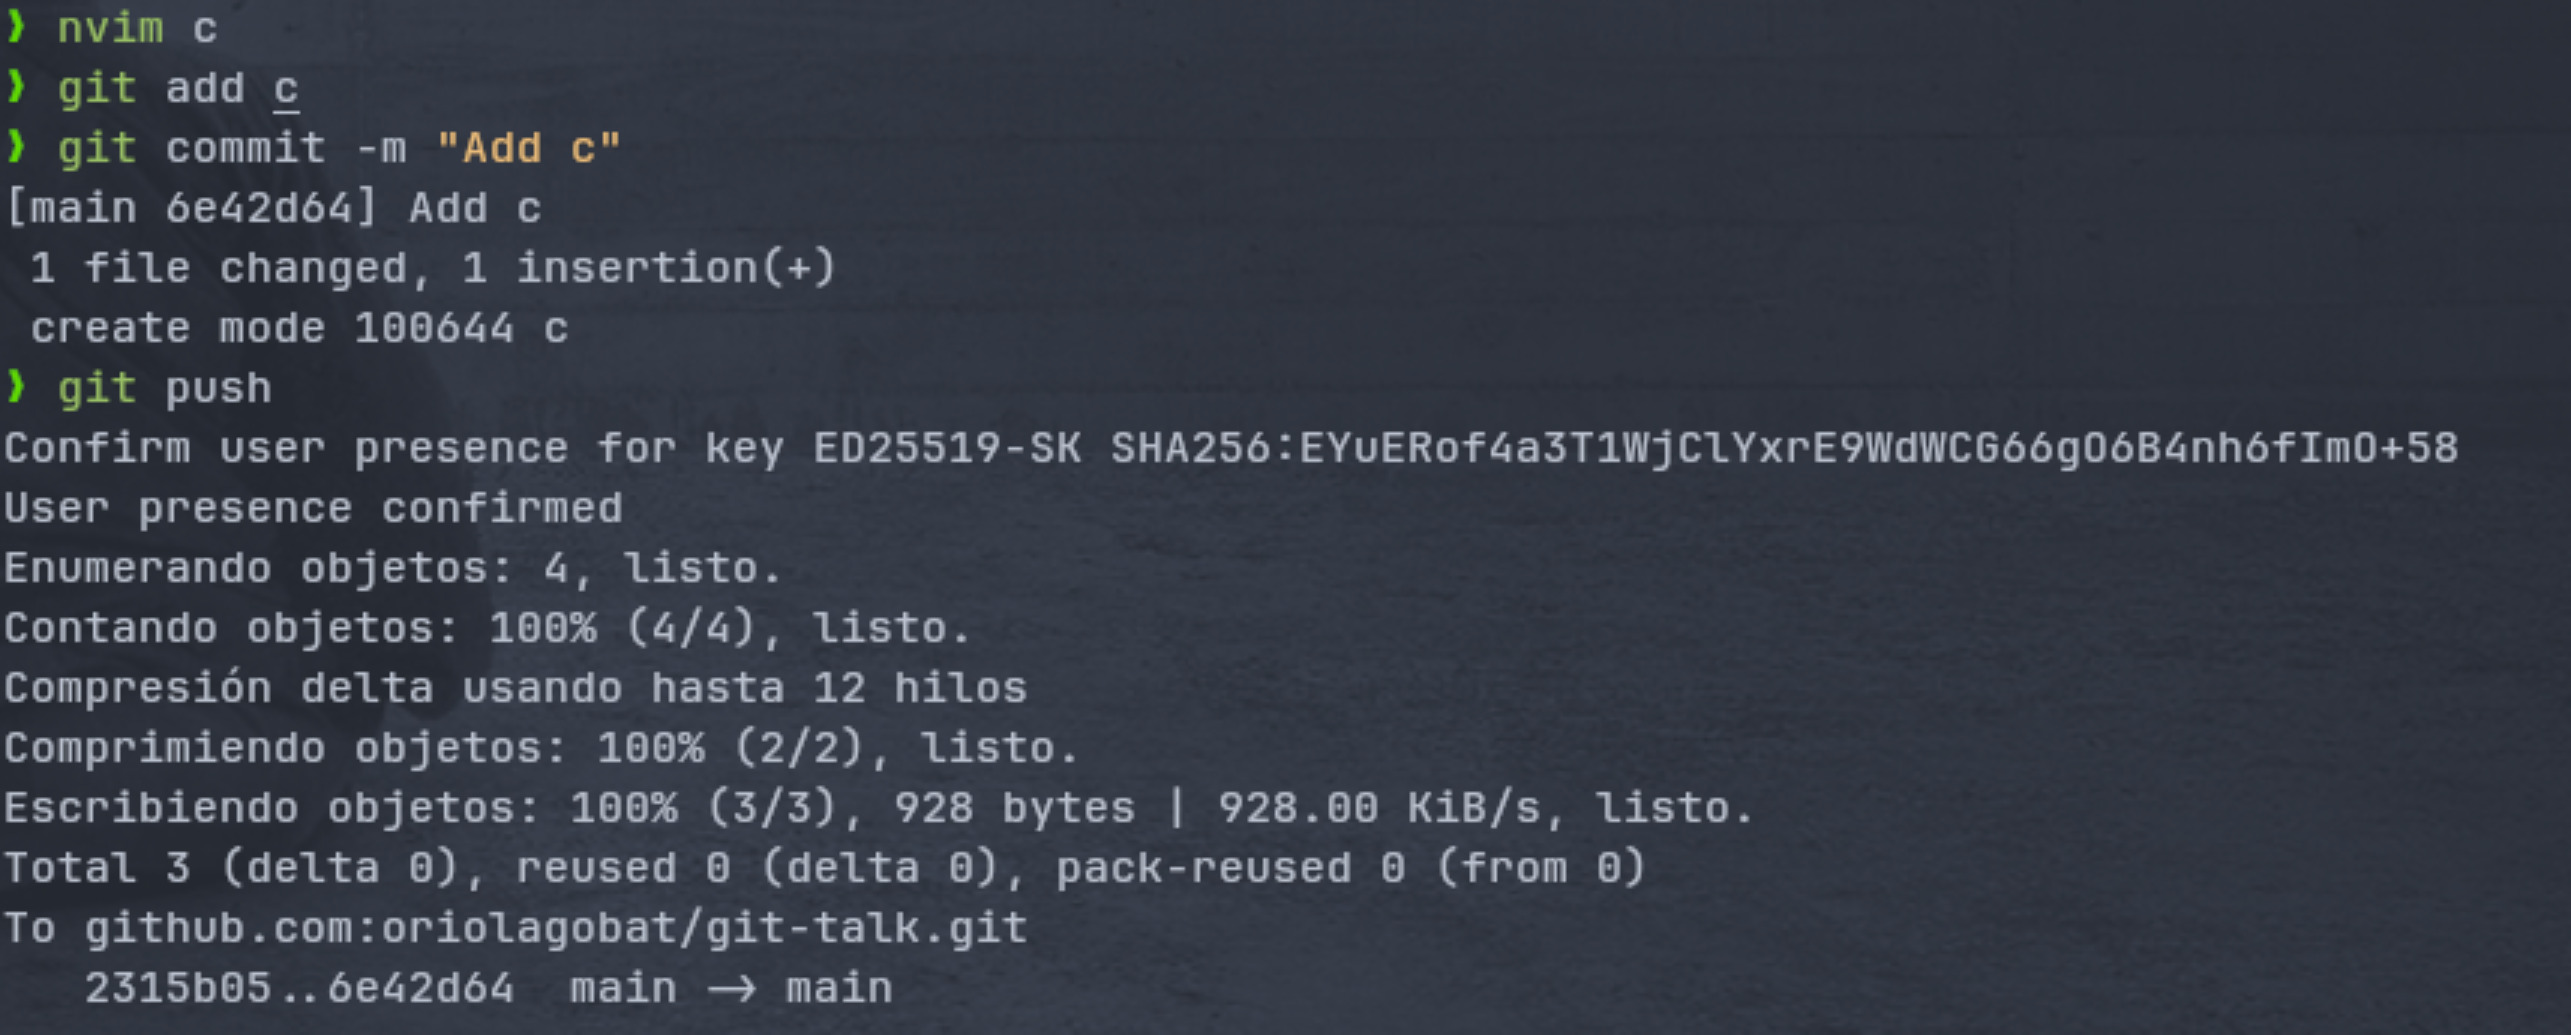
\includegraphics[scale=0.1]{images/com12}}
        \end{figure}
    \end{frame}


    \section{Mid}\label{sec:mid}

    \subsection{Log and resets}\label{subsec:log-and-resets}
    \begin{frame}
        \frametitle{Log and resets}
        \begin{figure}[H]
            \centering
            \noindent
            \makebox[\textwidth]{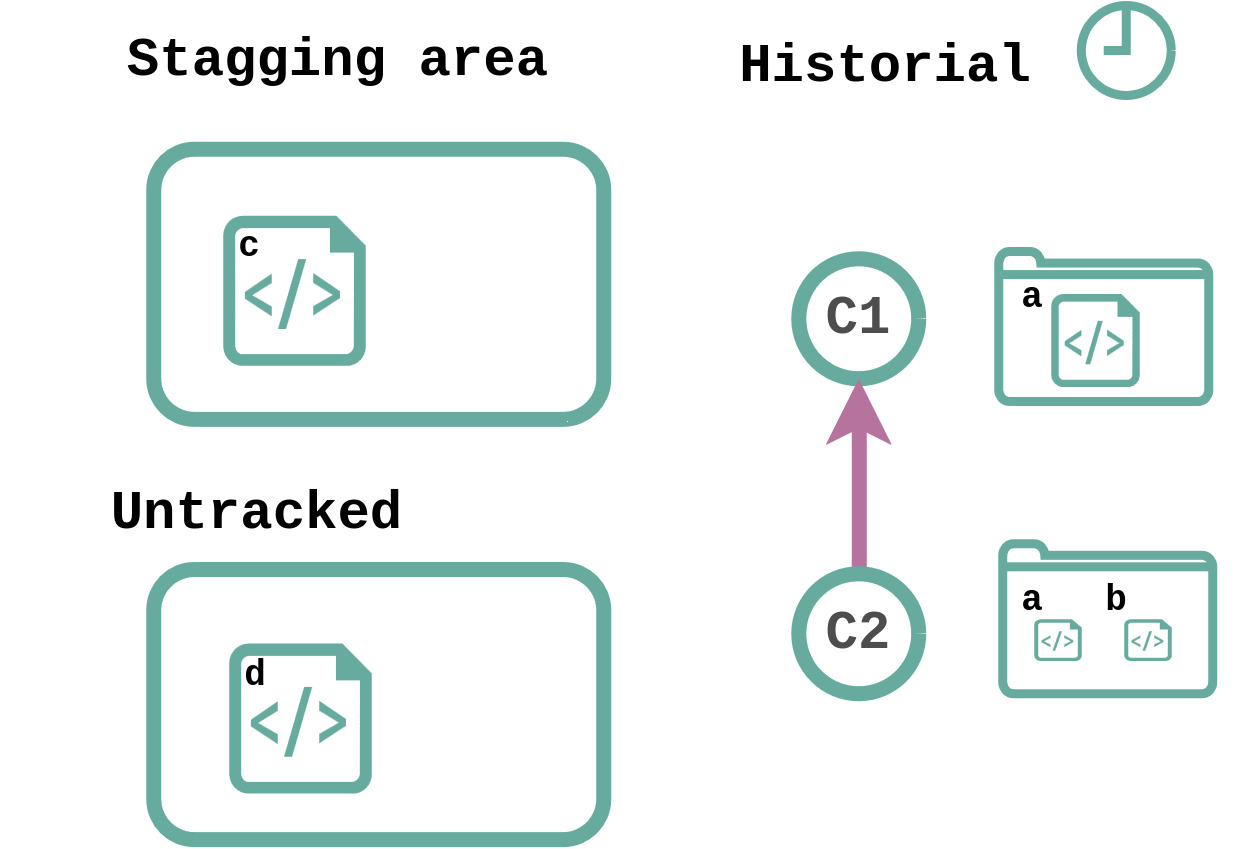
\includegraphics[scale=0.15]{images/log}}
        \end{figure}
    \end{frame}
    \begin{frame}
        \frametitle{Log and resets}
        \begin{itemize}
            \item \texttt{git log}: Show the commit history
            \item \texttt{git checkout <commit>}: Move the HEAD to the specified commit
            \item \texttt{git reset --hard <commit>}: Move the HEAD to the specified commit and reset the working directory
            \item \texttt{git reset --soft <commit>}: Move the HEAD to the specified commit and keep the working directory
        \end{itemize}
    \end{frame}
    \begin{frame}
        \frametitle{Log and resets}
        \begin{figure}[H]
            \centering
            \noindent
            \makebox[\textwidth]{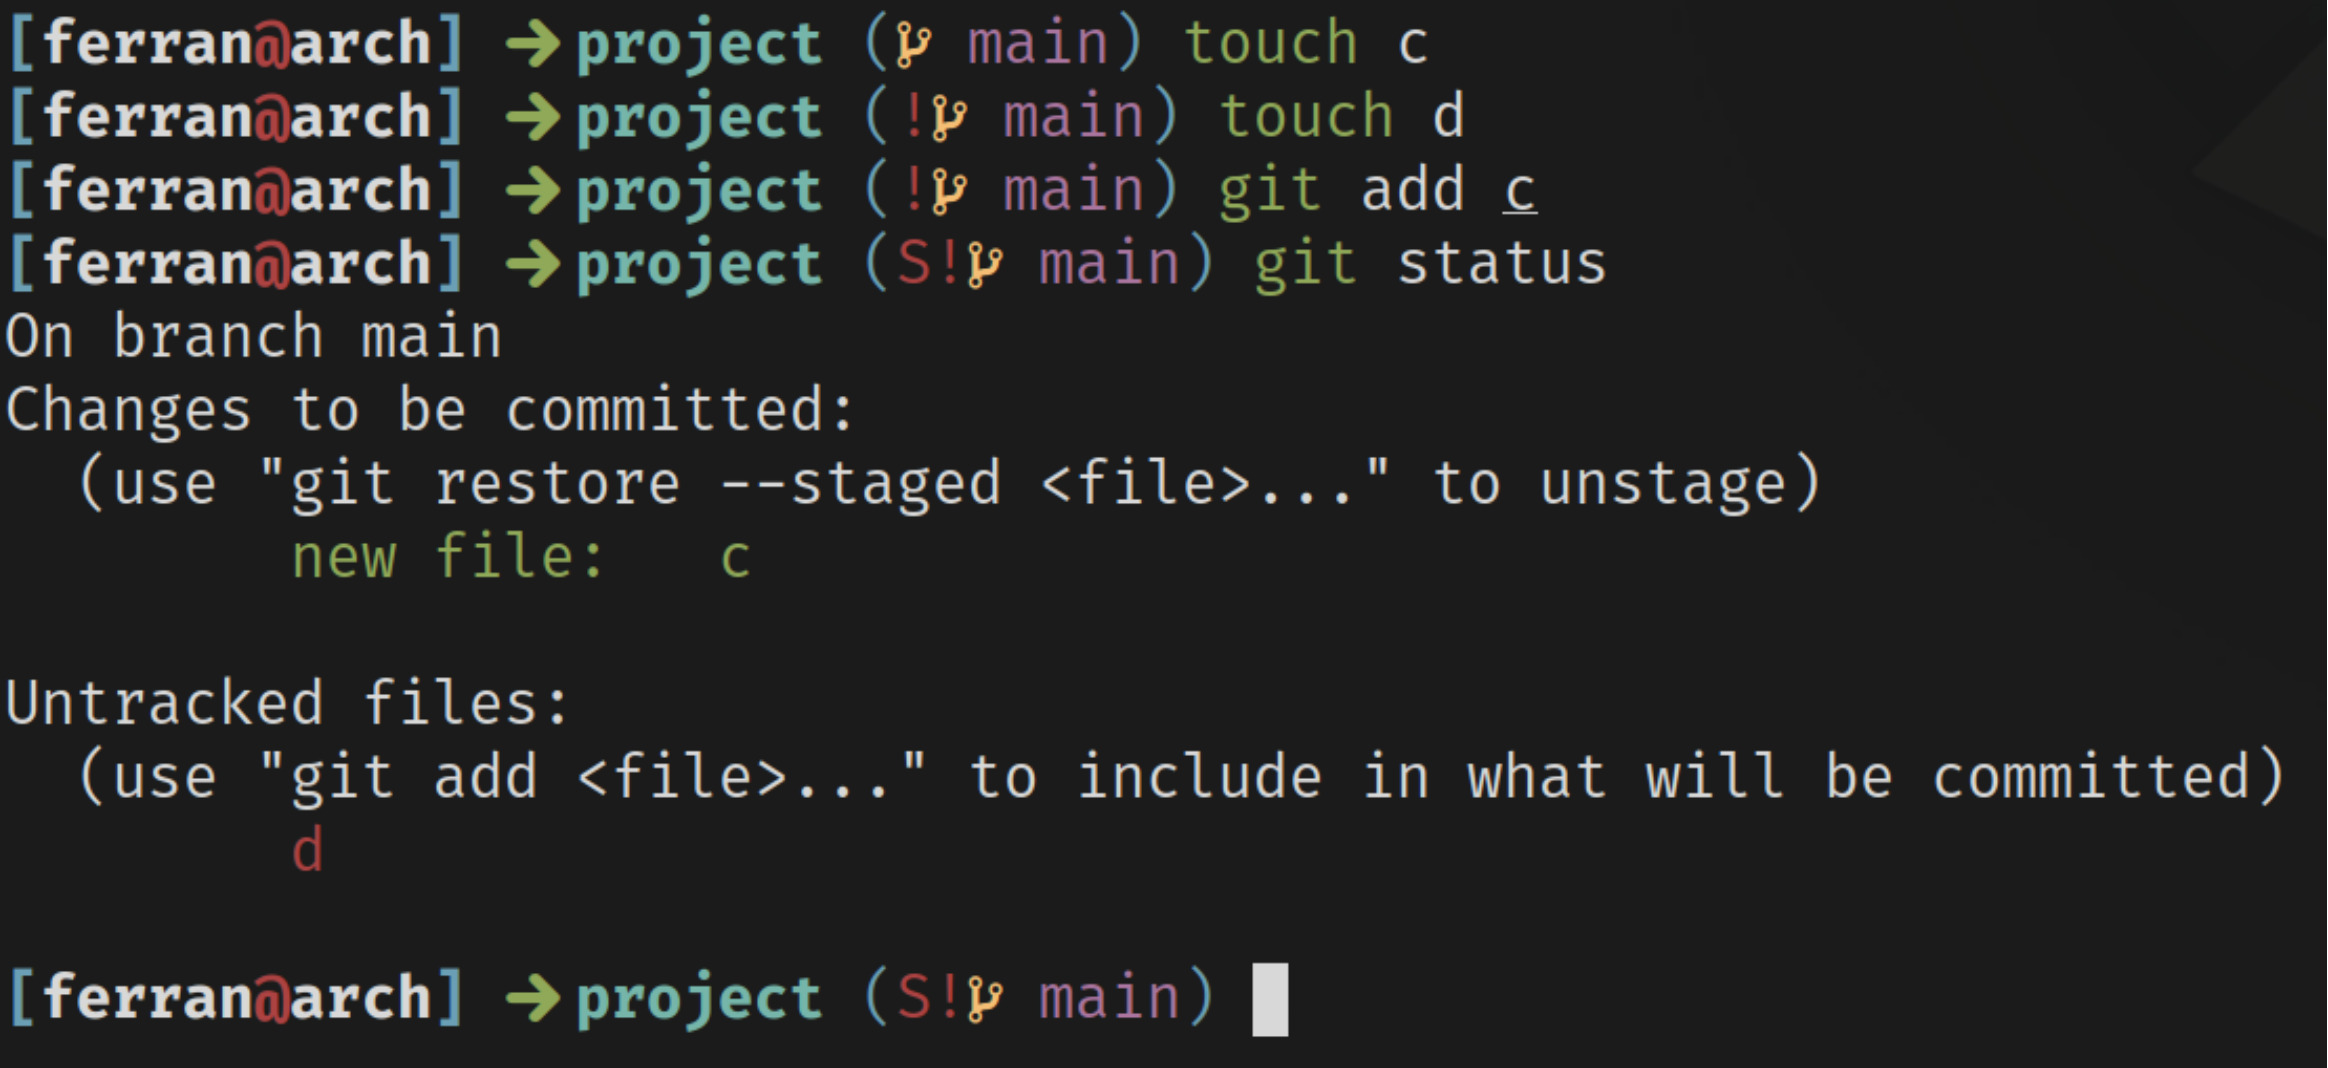
\includegraphics[scale=0.15]{images/com20}}
        \end{figure}
    \end{frame}
    \begin{frame}
        \frametitle{Log and resets}
        \begin{figure}[H]
            \centering
            \noindent
            \makebox[\textwidth]{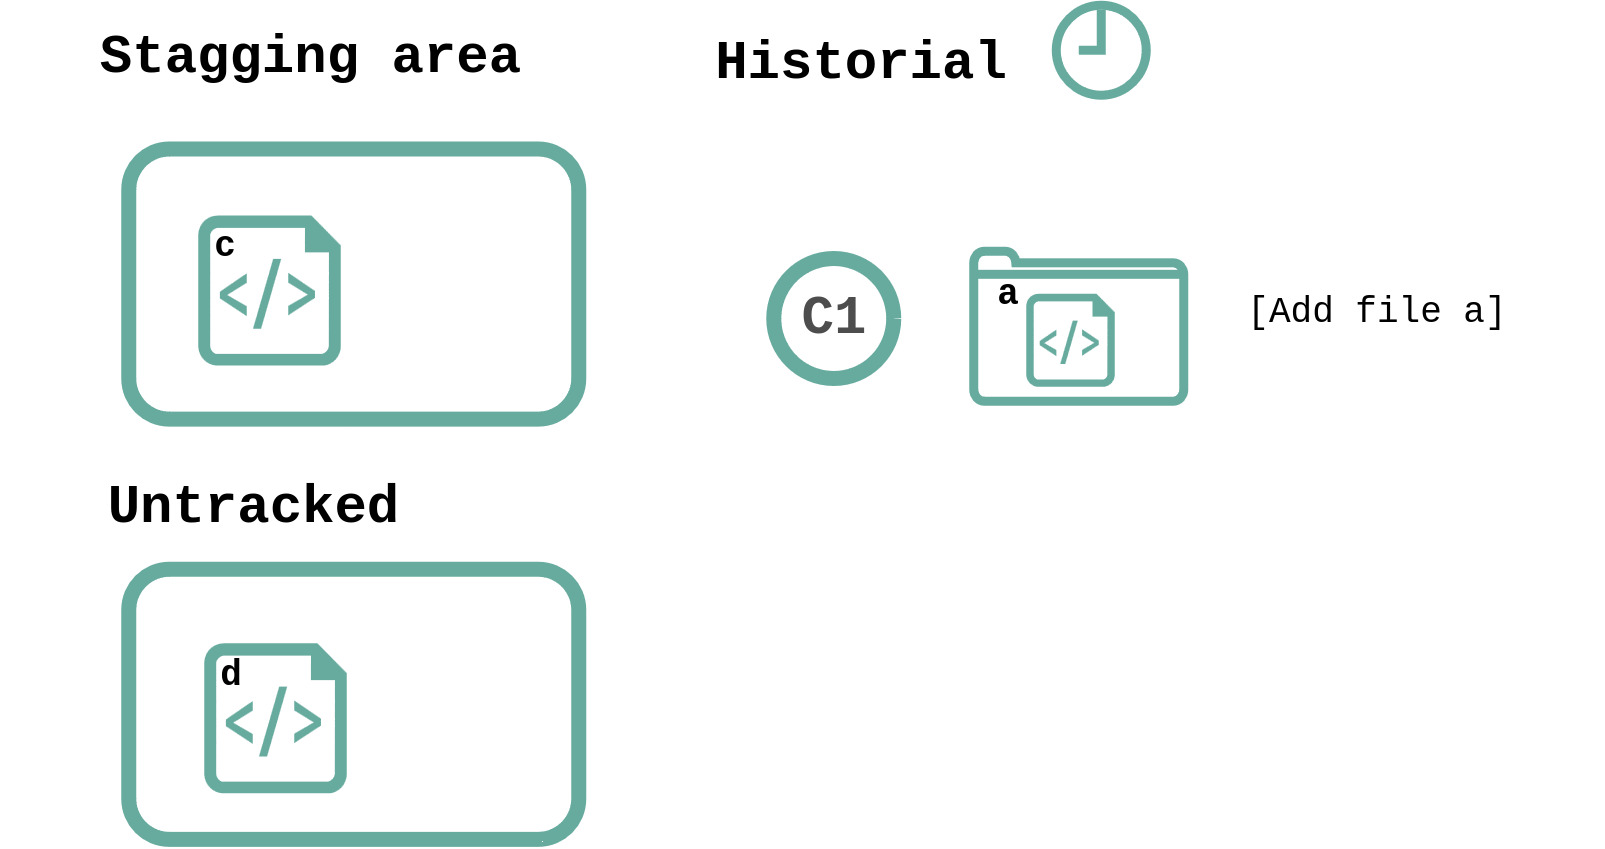
\includegraphics[scale=0.15]{images/log-2}}
        \end{figure}
    \end{frame}
    \begin{frame}
        \frametitle{Log and resets}
        \begin{figure}[H]
            \centering
            \noindent
            \makebox[\textwidth]{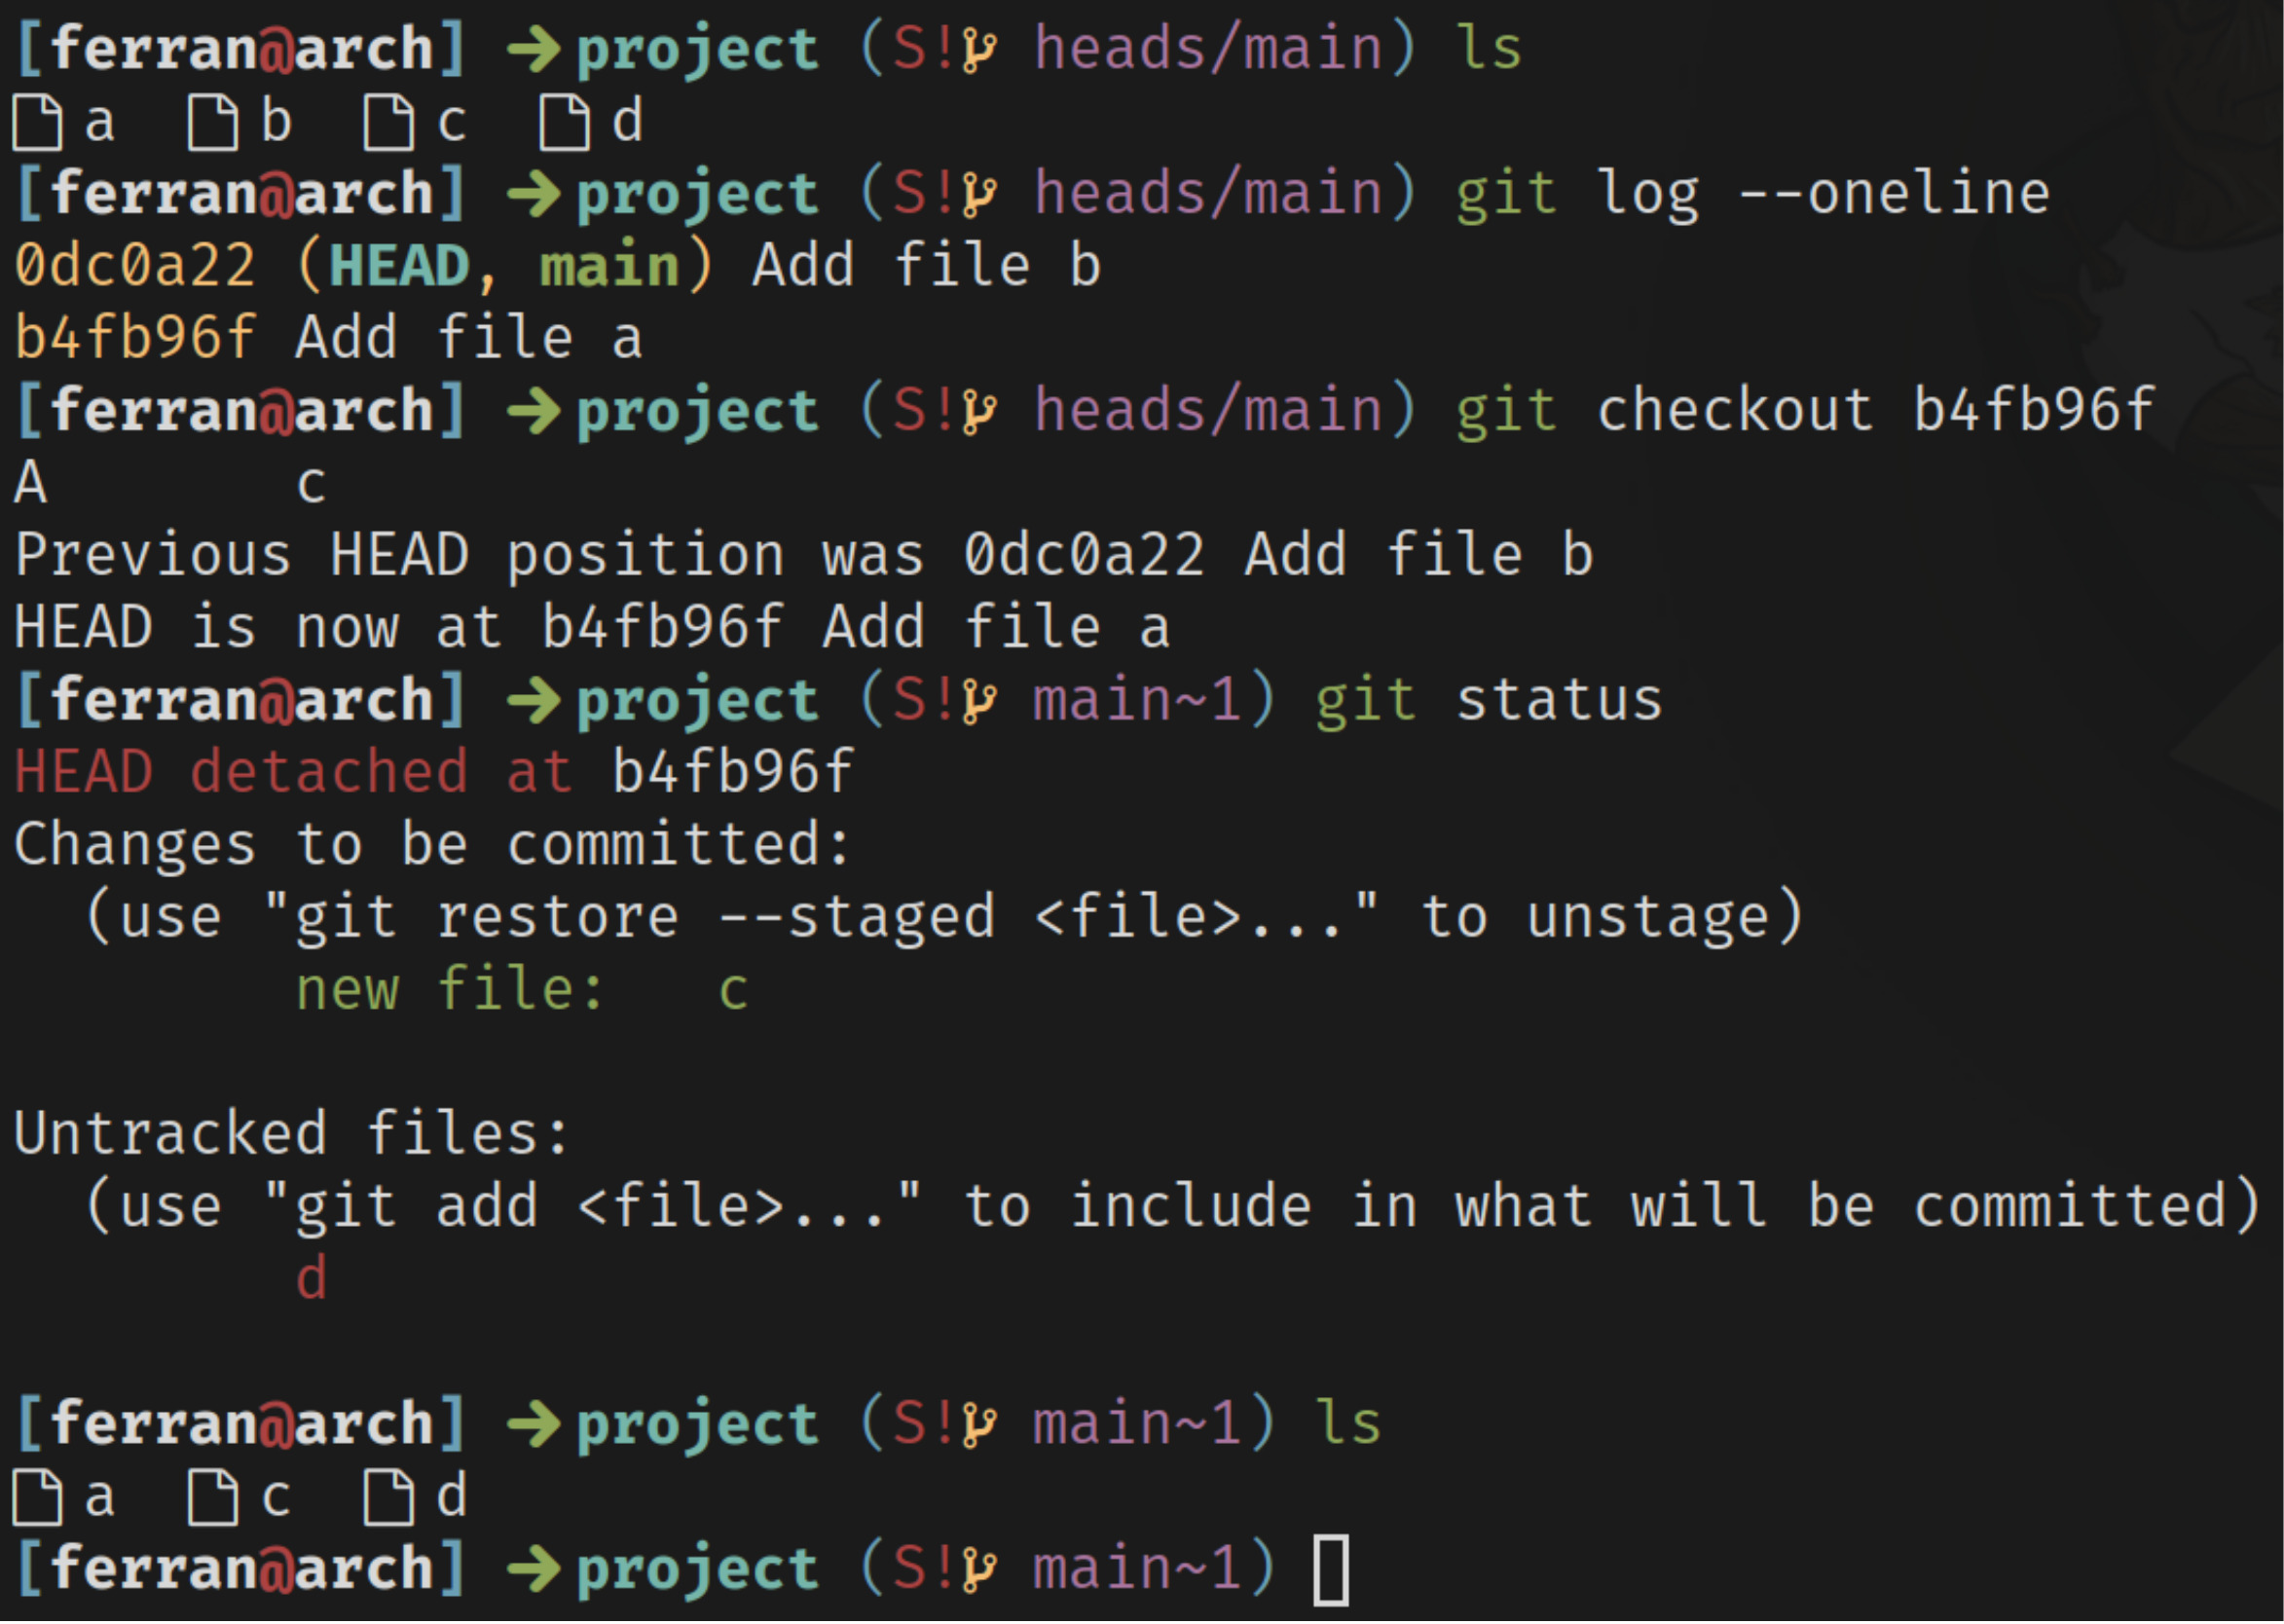
\includegraphics[scale=0.10]{images/com21}}
        \end{figure}
    \end{frame}
    \begin{frame}
        \frametitle{Log and resets}
        \begin{figure}[H]
            \centering
            \noindent
            \makebox[\textwidth]{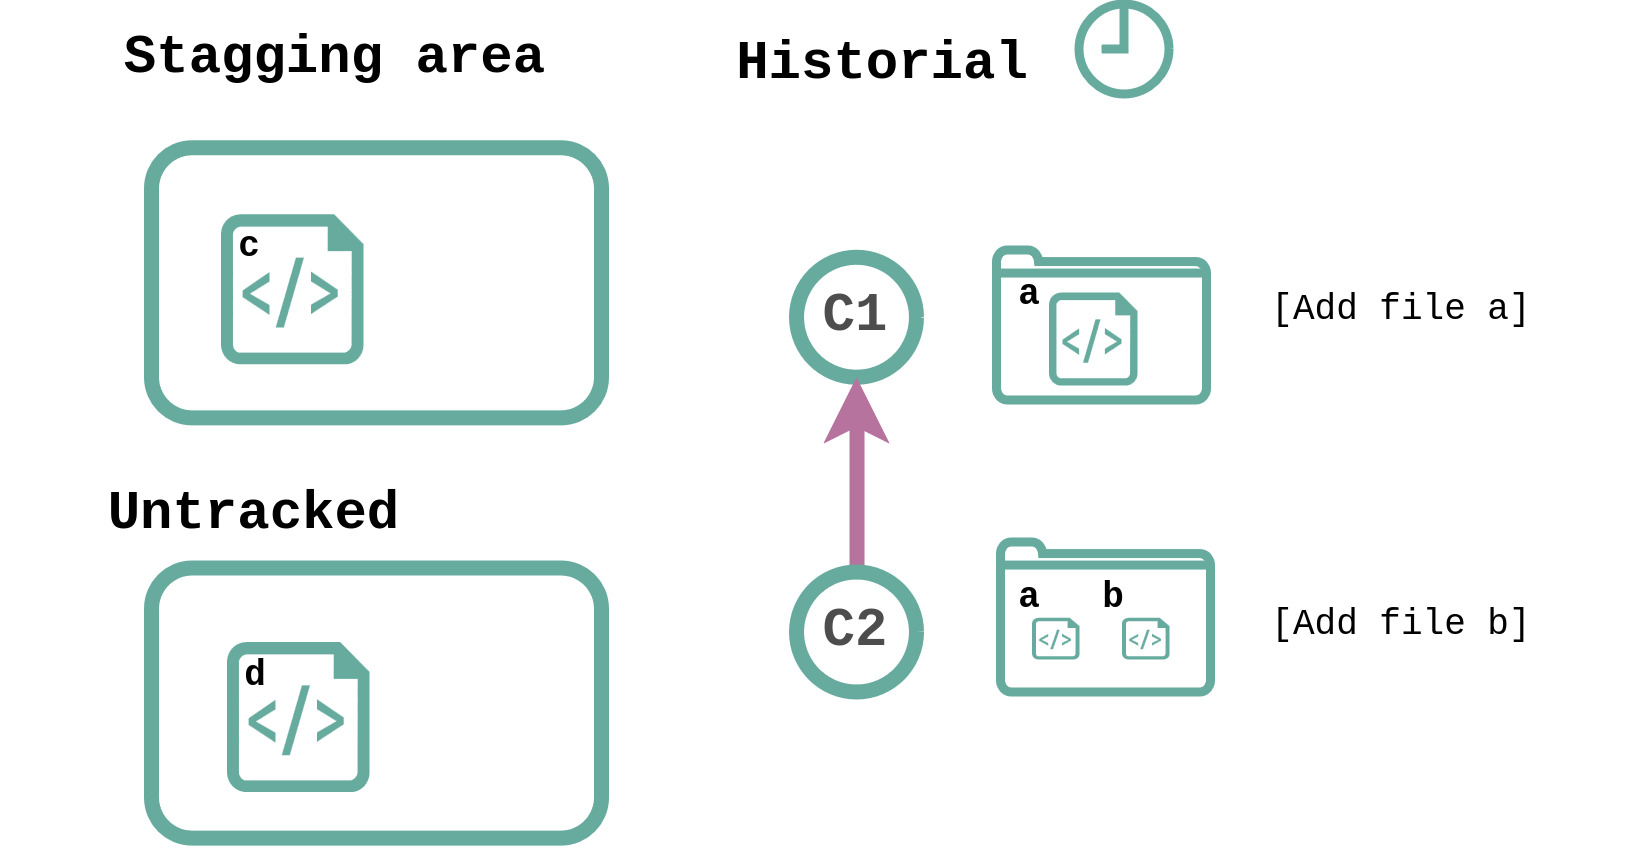
\includegraphics[scale=0.15]{images/log-3}}
        \end{figure}
    \end{frame}
    \begin{frame}
        \frametitle{Log and resets}
        \begin{figure}[H]
            \centering
            \noindent
            \makebox[\textwidth]{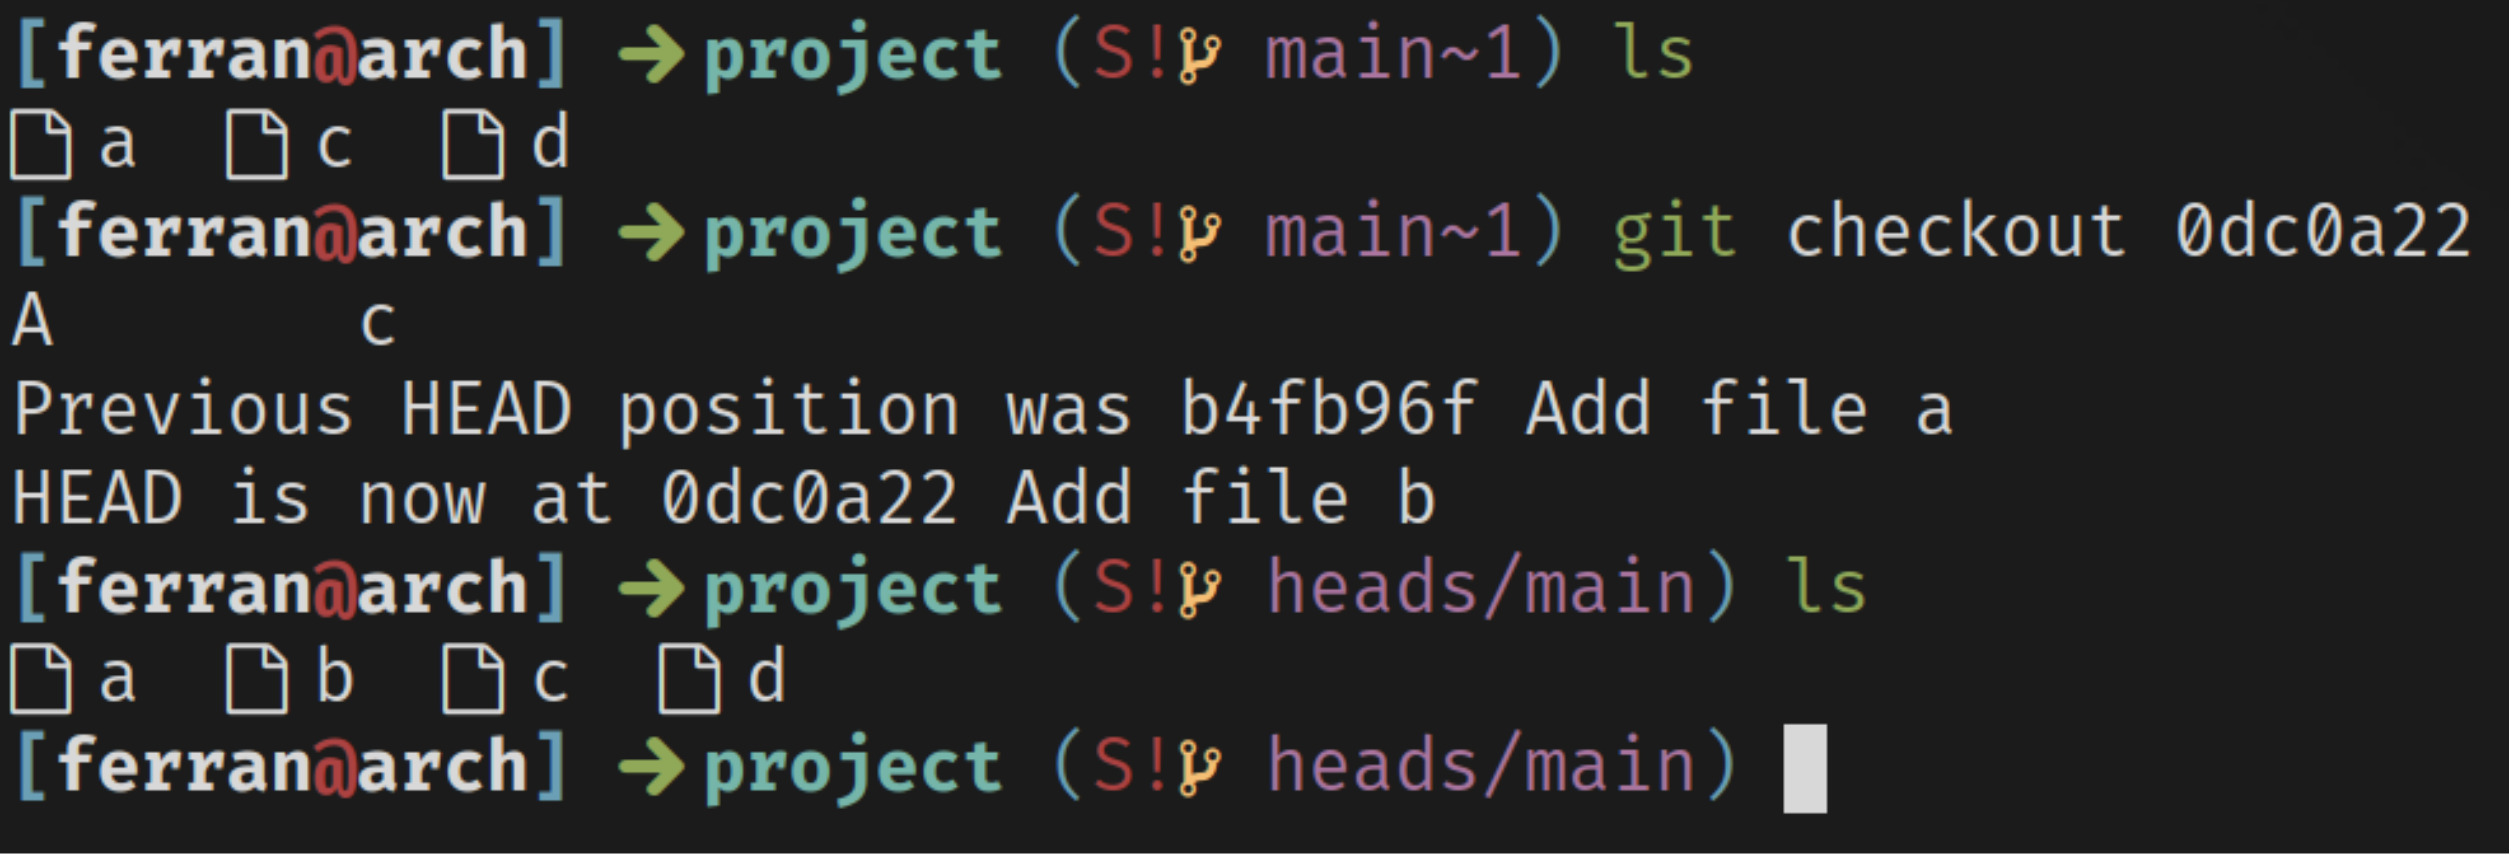
\includegraphics[scale=0.1]{images/com23}}
        \end{figure}
    \end{frame}
    \begin{frame}
        \frametitle{Log and resets}
        \begin{figure}[H]
            \centering
            \noindent
            \makebox[\textwidth]{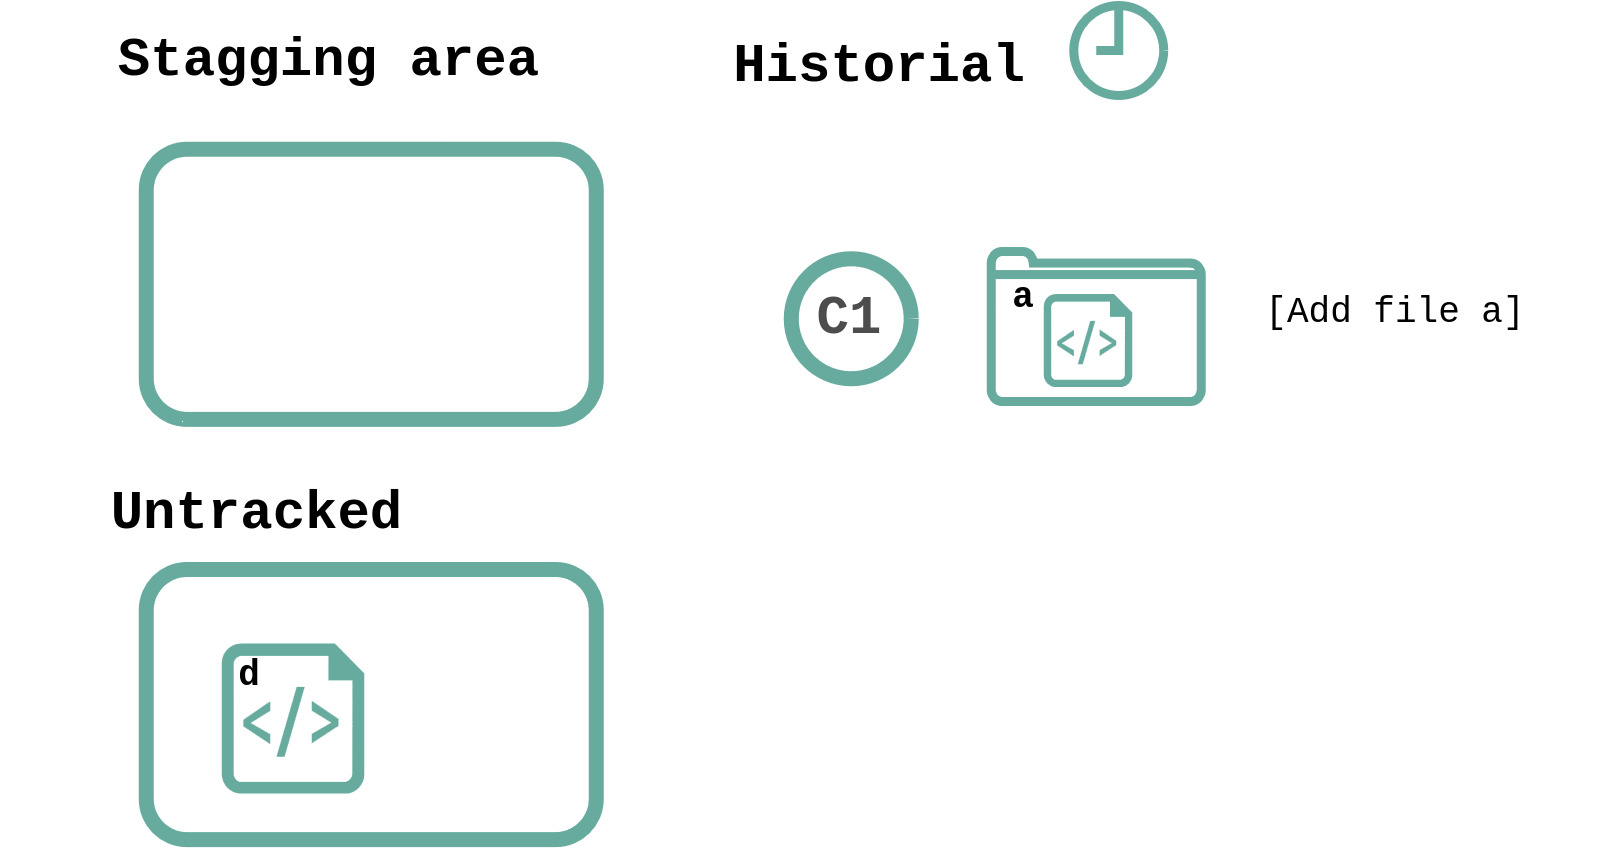
\includegraphics[scale=0.15]{images/log-4}}
        \end{figure}
    \end{frame}
    \begin{frame}
        \frametitle{Log and resets}
        \begin{figure}[H]
            \centering
            \noindent
            \makebox[\textwidth]{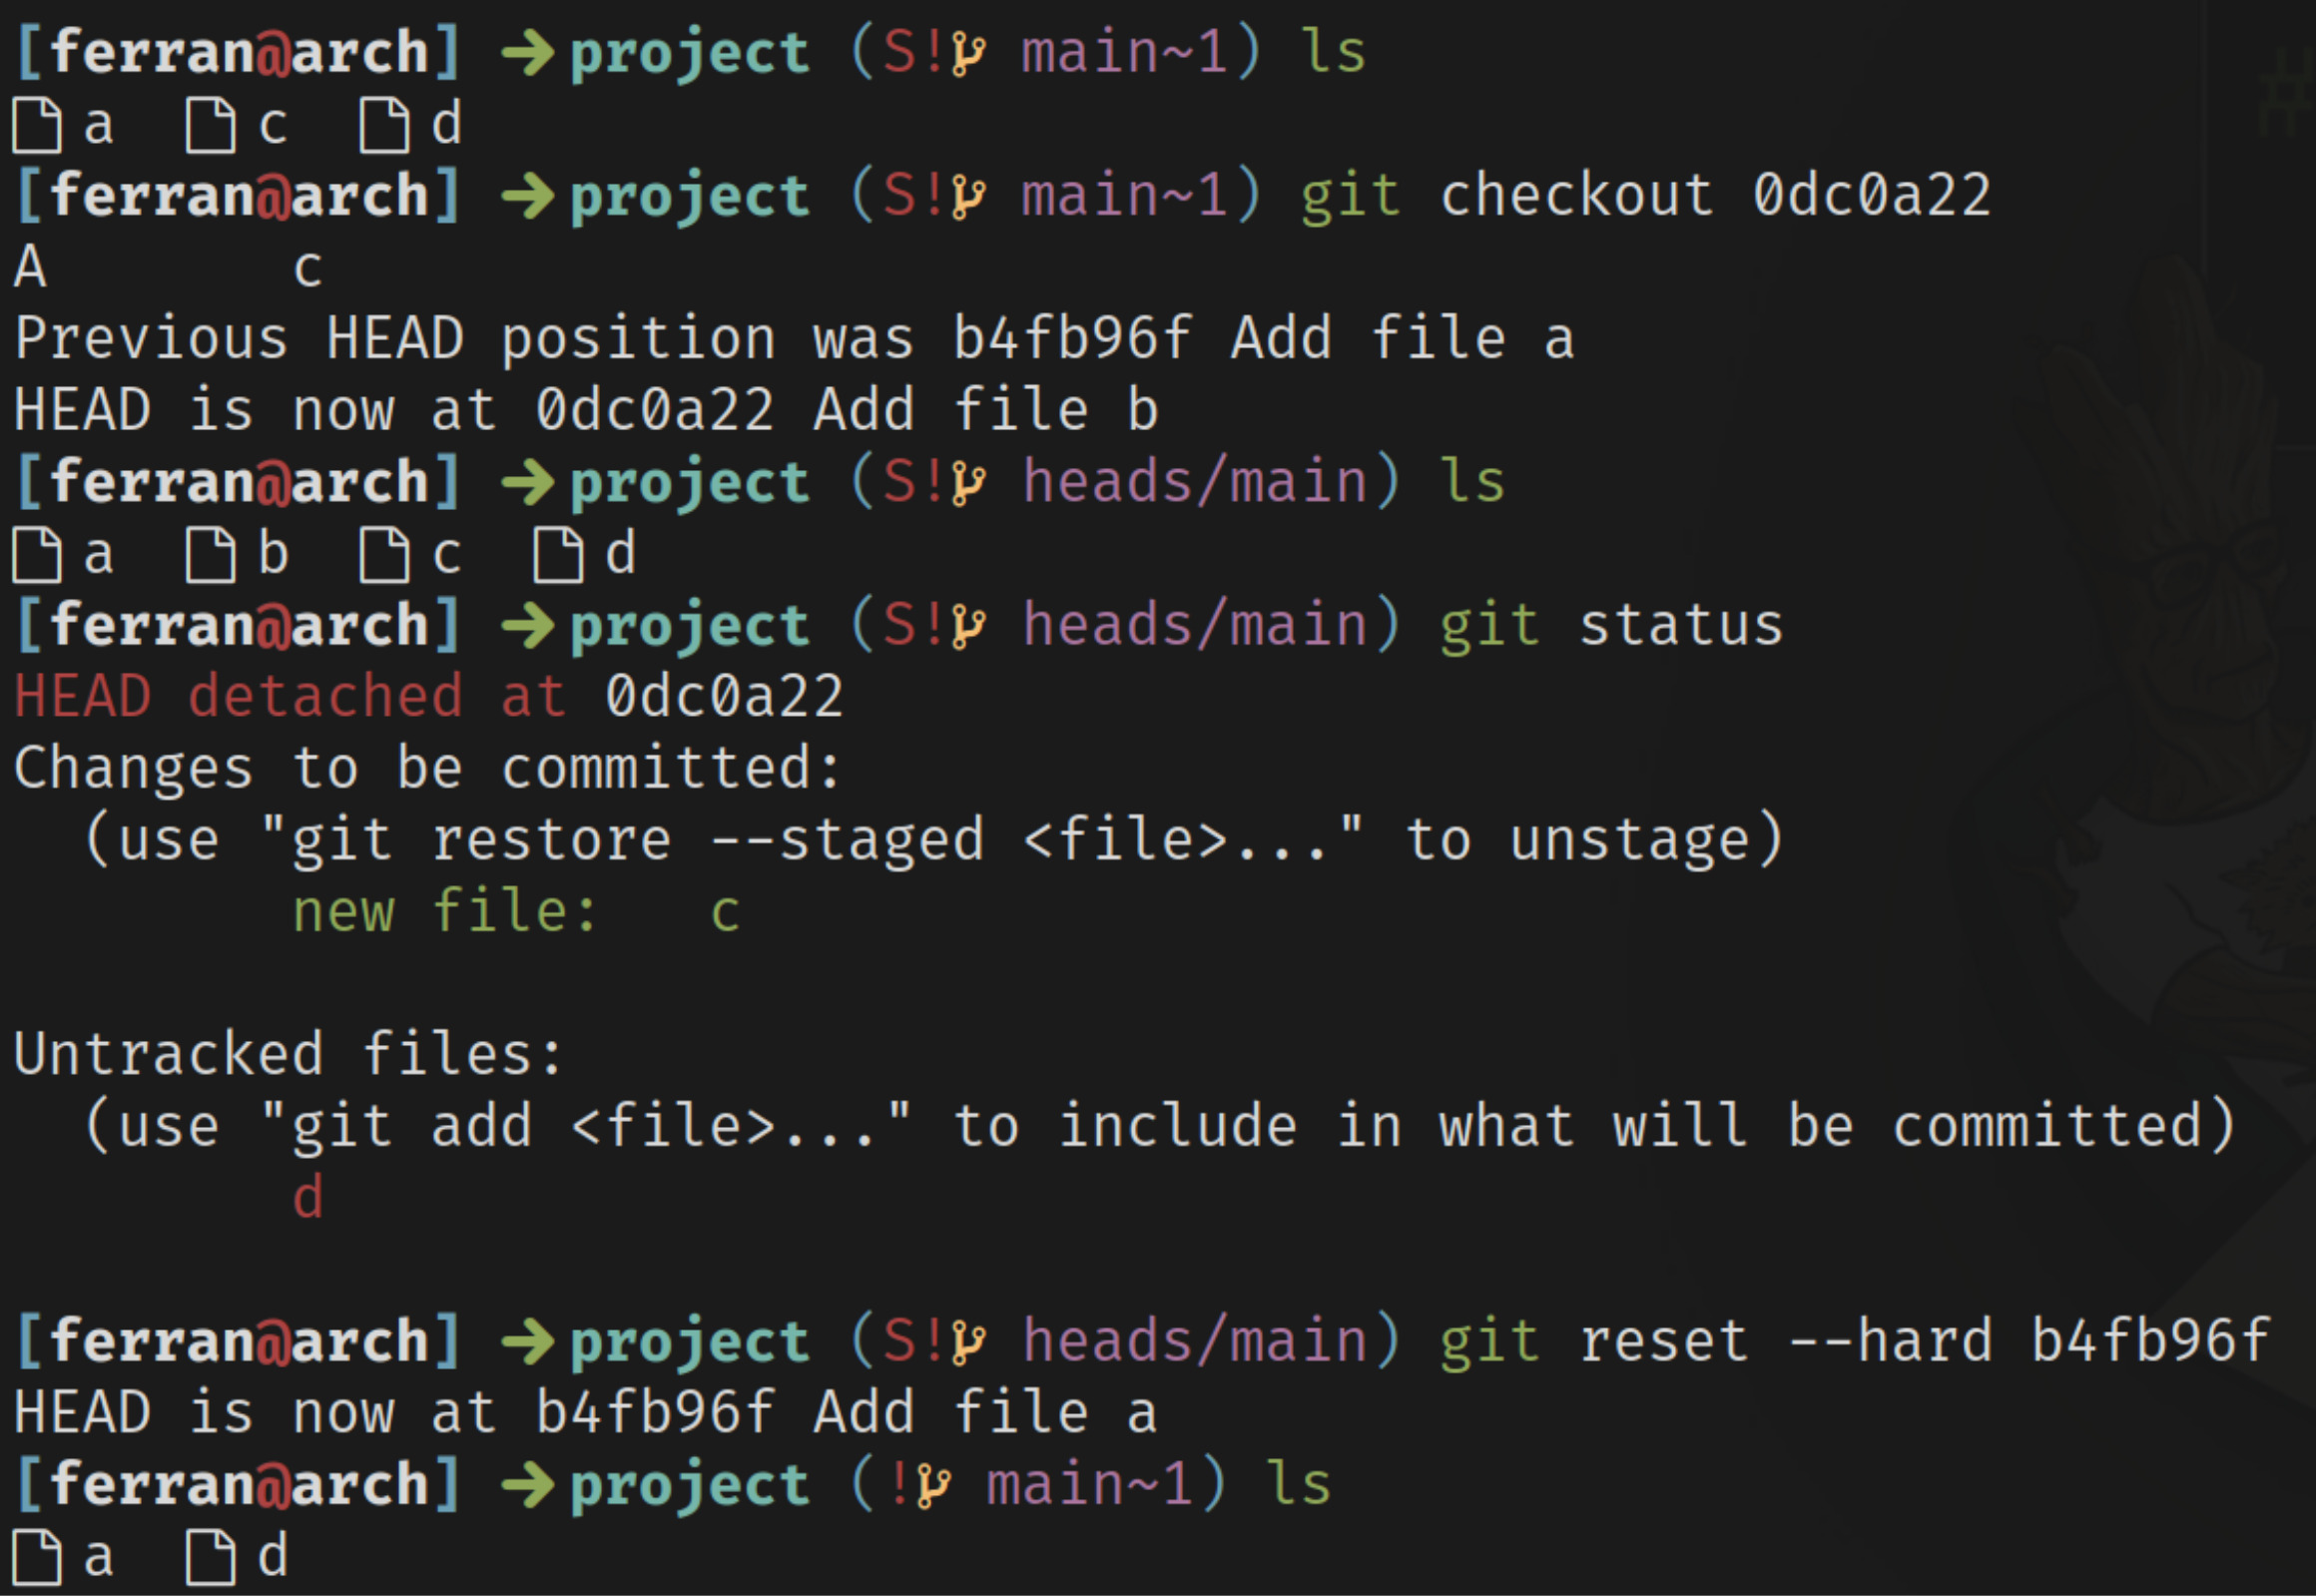
\includegraphics[scale=0.08]{images/com24}}
        \end{figure}
    \end{frame}

    \subsection{Branches}\label{subsec:branches}
    \begin{frame}
        \frametitle{Branches}
        \begin{figure}[H]
            \centering
            \noindent
            \makebox[\textwidth]{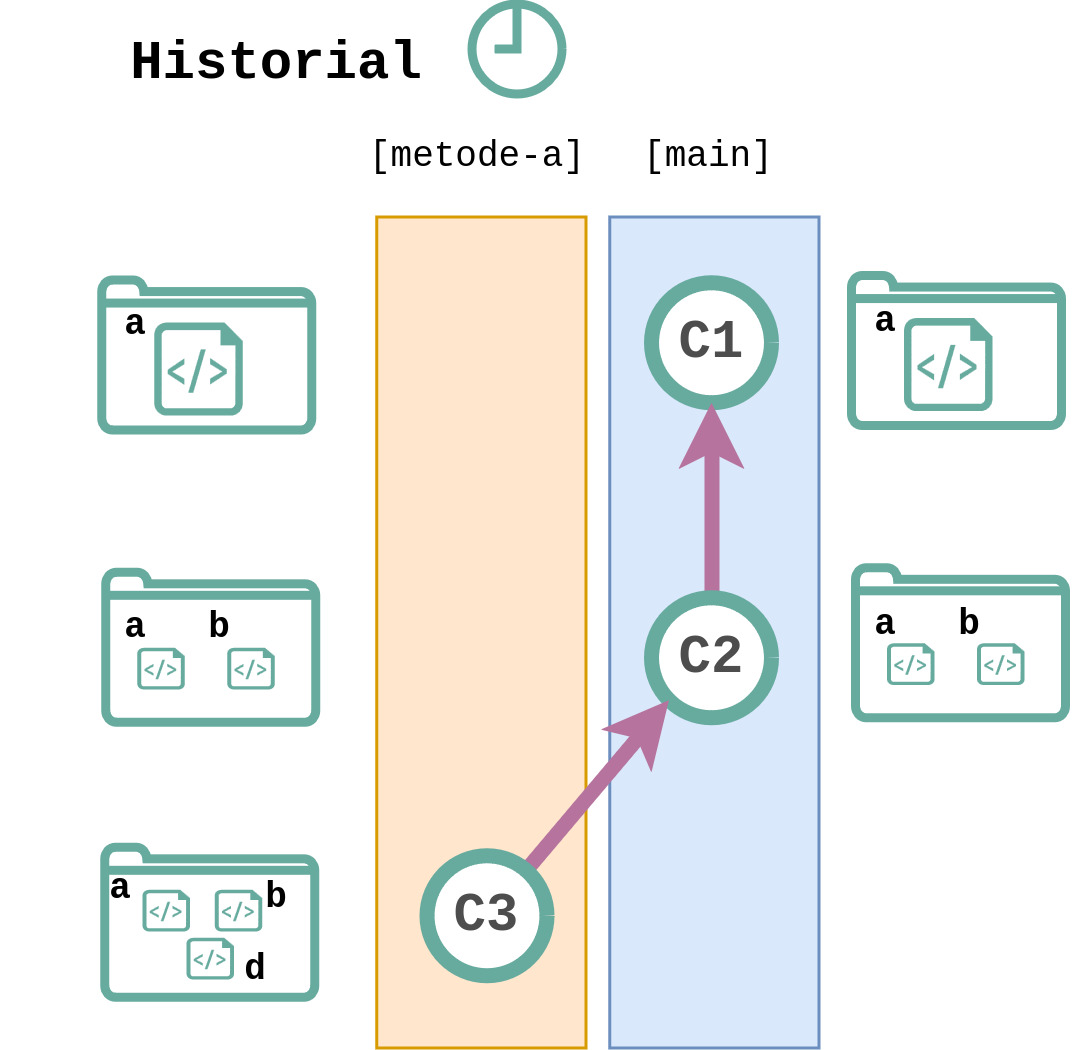
\includegraphics[scale=0.15]{images/branch1}}
        \end{figure}
    \end{frame}
    \begin{frame}
        \frametitle{Branches}
        \begin{itemize}
            \item \texttt{git branch}: List the branches
            \item \texttt{git checkout -b <branch>}: Create a new branch and switch to it
            \item \texttt{git checkout}: Switch to another branch
        \end{itemize}
    \end{frame}
    \begin{frame}
        \frametitle{Branches}
        \begin{figure}[H]
            \centering
            \noindent
            \makebox[\textwidth]{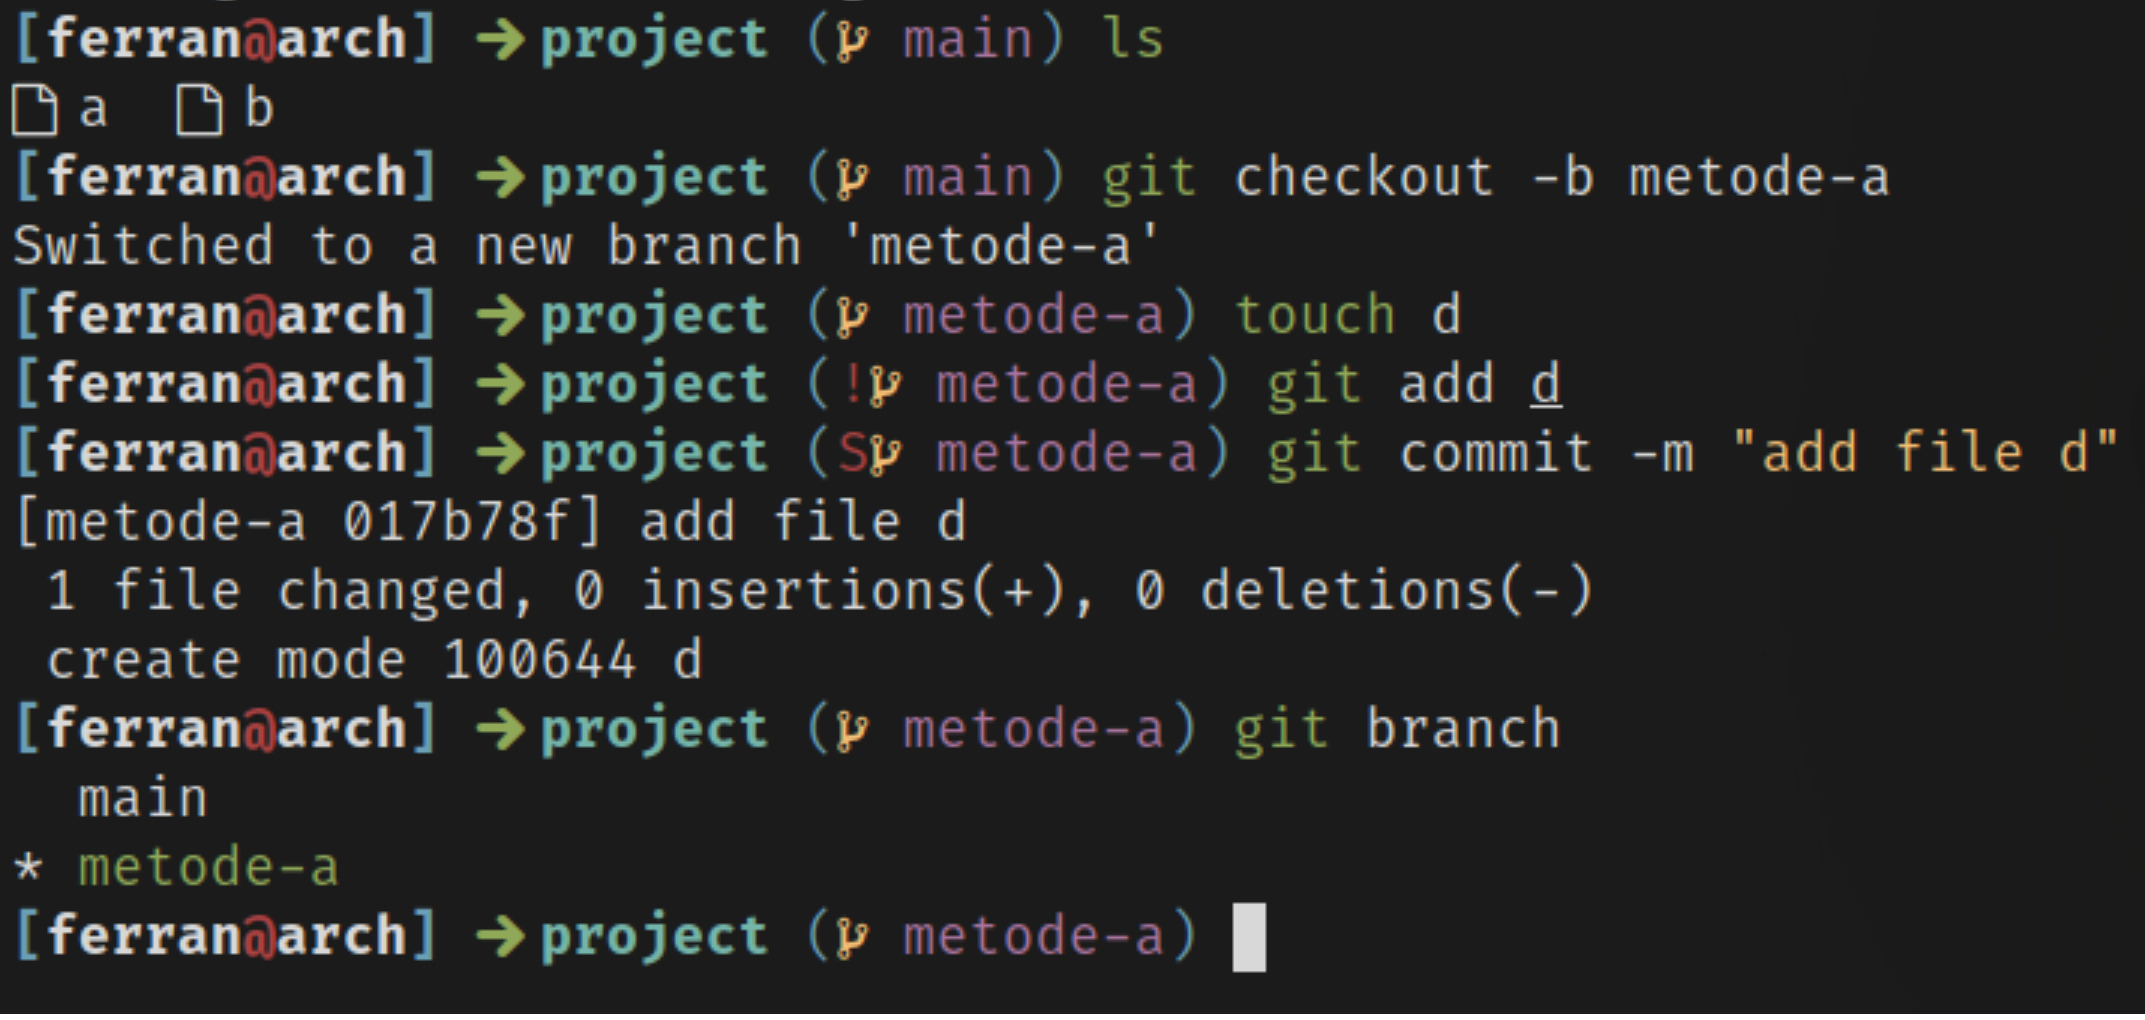
\includegraphics[scale=0.15]{images/branch-com-1}}
        \end{figure}
    \end{frame}
    \begin{frame}
        \frametitle{Branches}
        \begin{figure}[H]
            \centering
            \noindent
            \makebox[\textwidth]{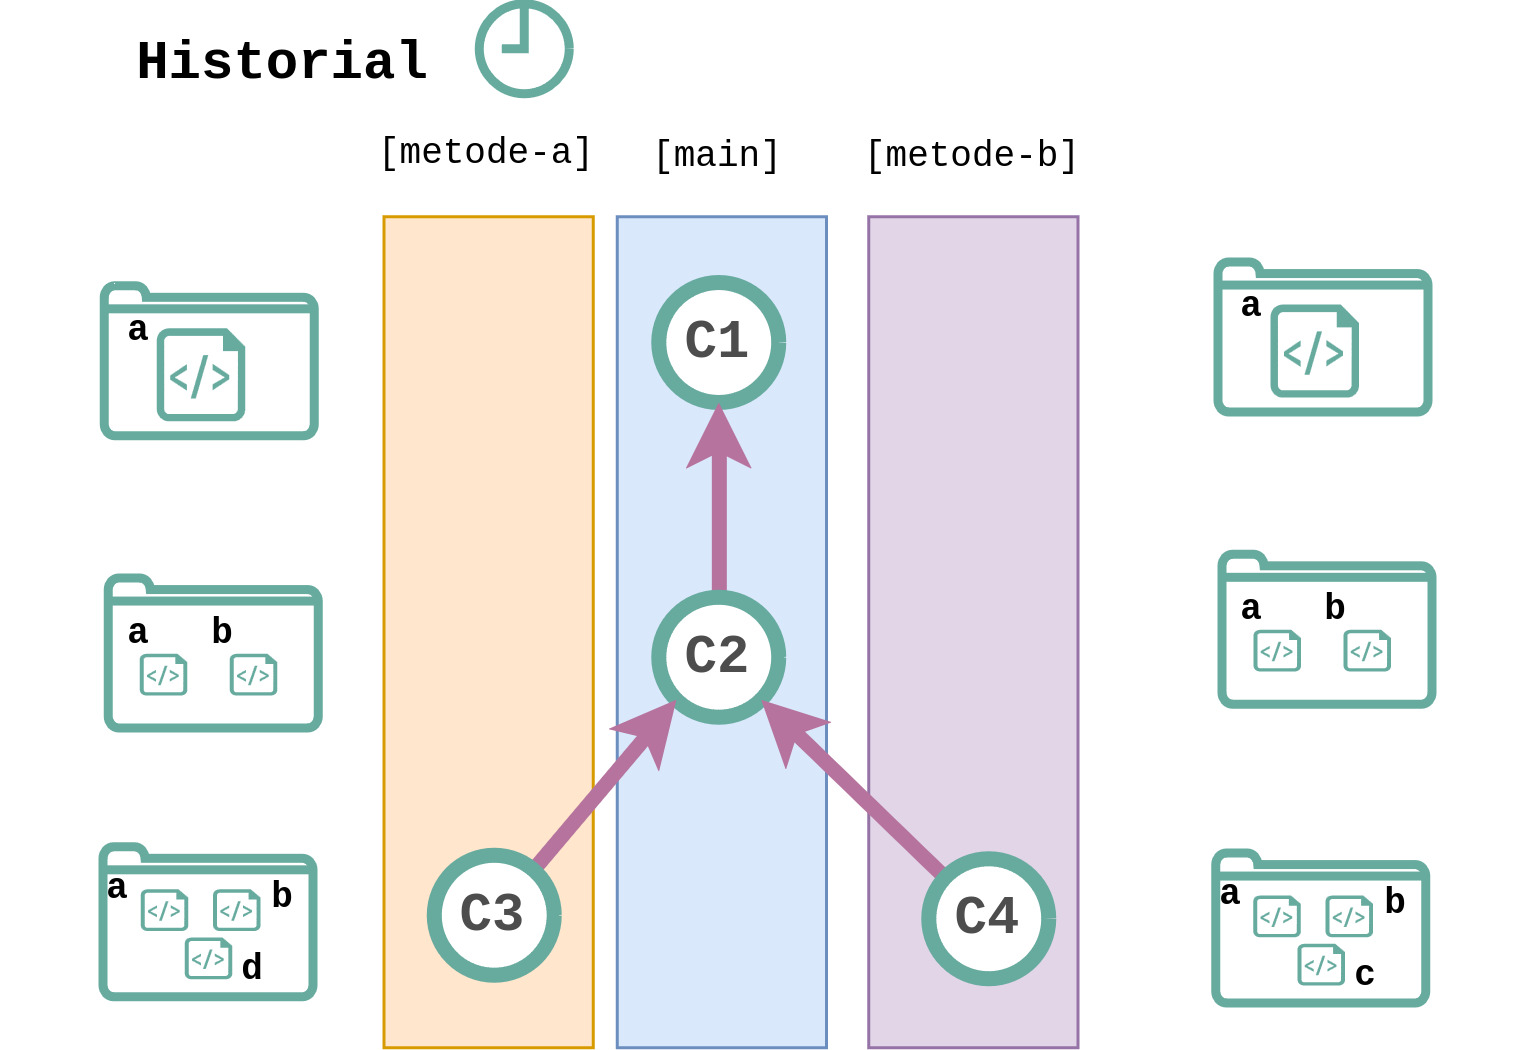
\includegraphics[scale=0.15]{images/branch2}}
        \end{figure}
    \end{frame}
    \begin{frame}
        \frametitle{Branches}
        \begin{figure}[H]
            \centering
            \noindent
            \makebox[\textwidth]{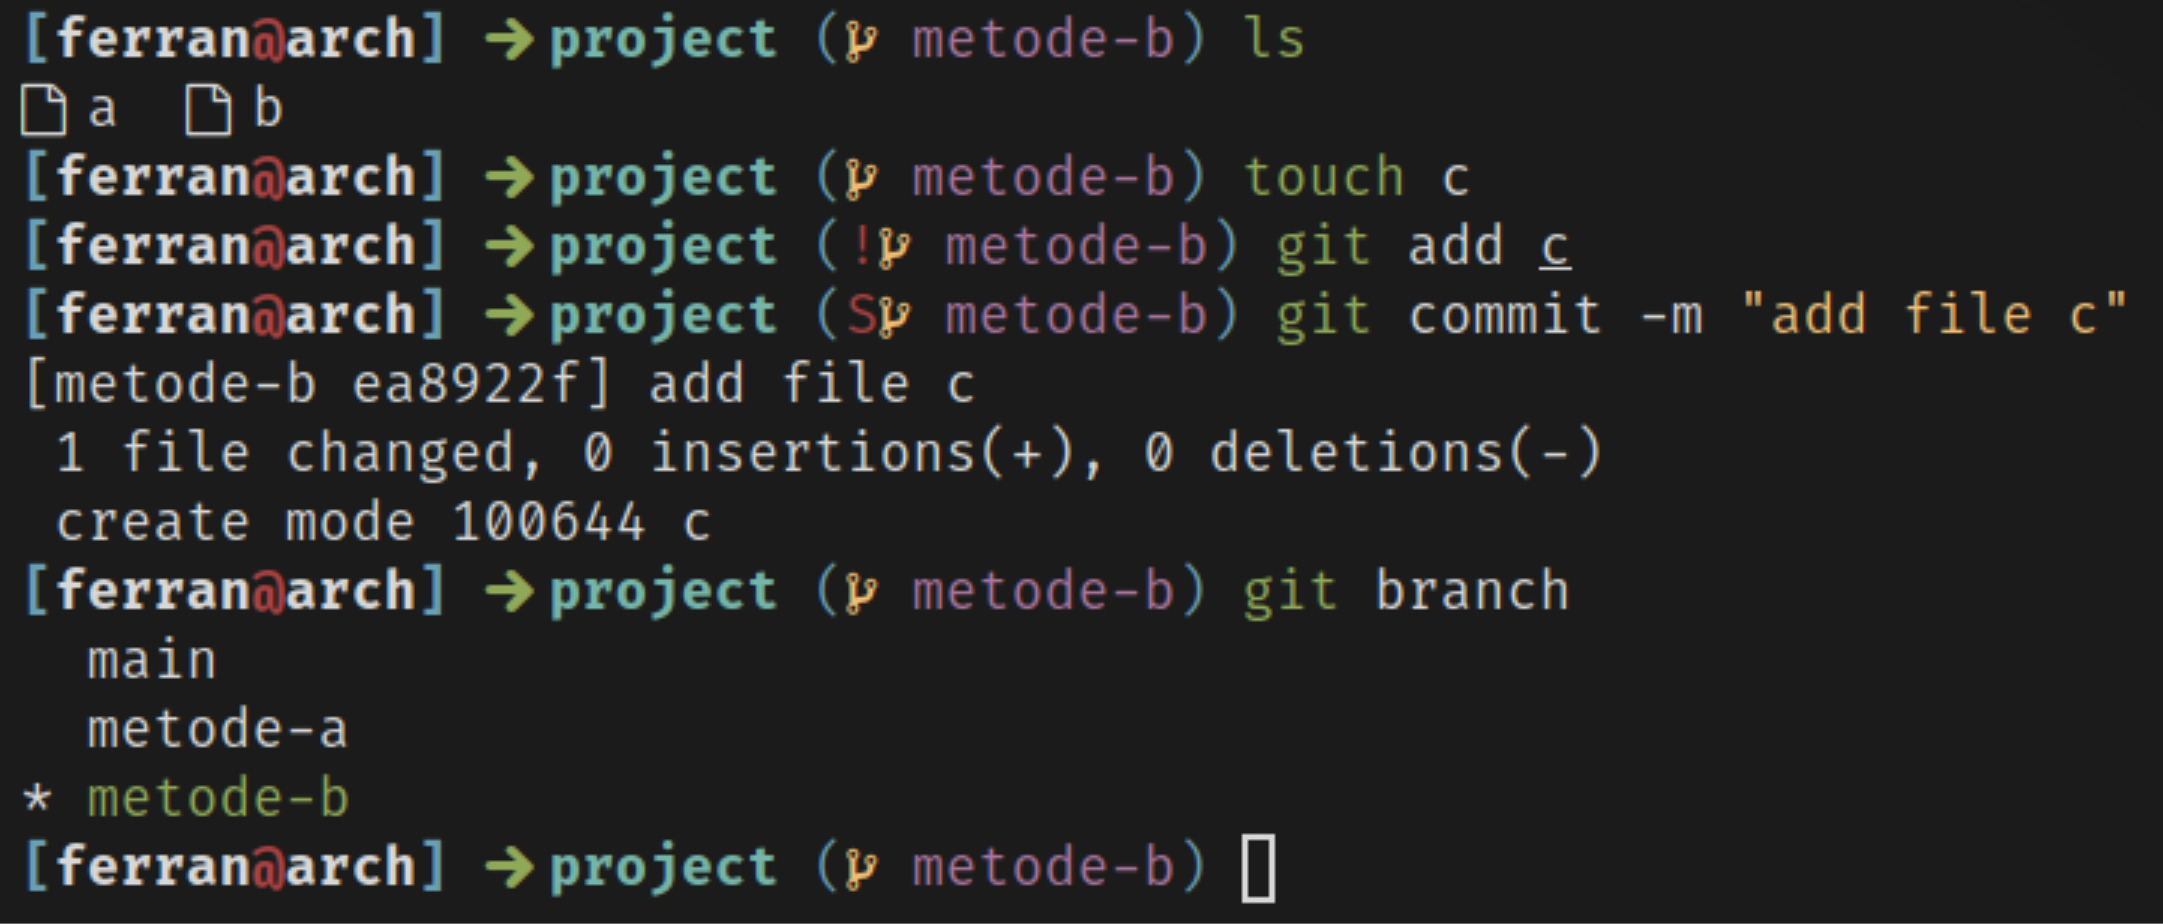
\includegraphics[scale=0.15]{images/branch-com2}}
        \end{figure}
    \end{frame}

    \subsection{Merge/rebase}\label{subsec:merge/rebase}
    \begin{frame}
        \frametitle{Merge and rebase}
        \begin{figure}[H]
            \centering
            \noindent
            \makebox[\textwidth]{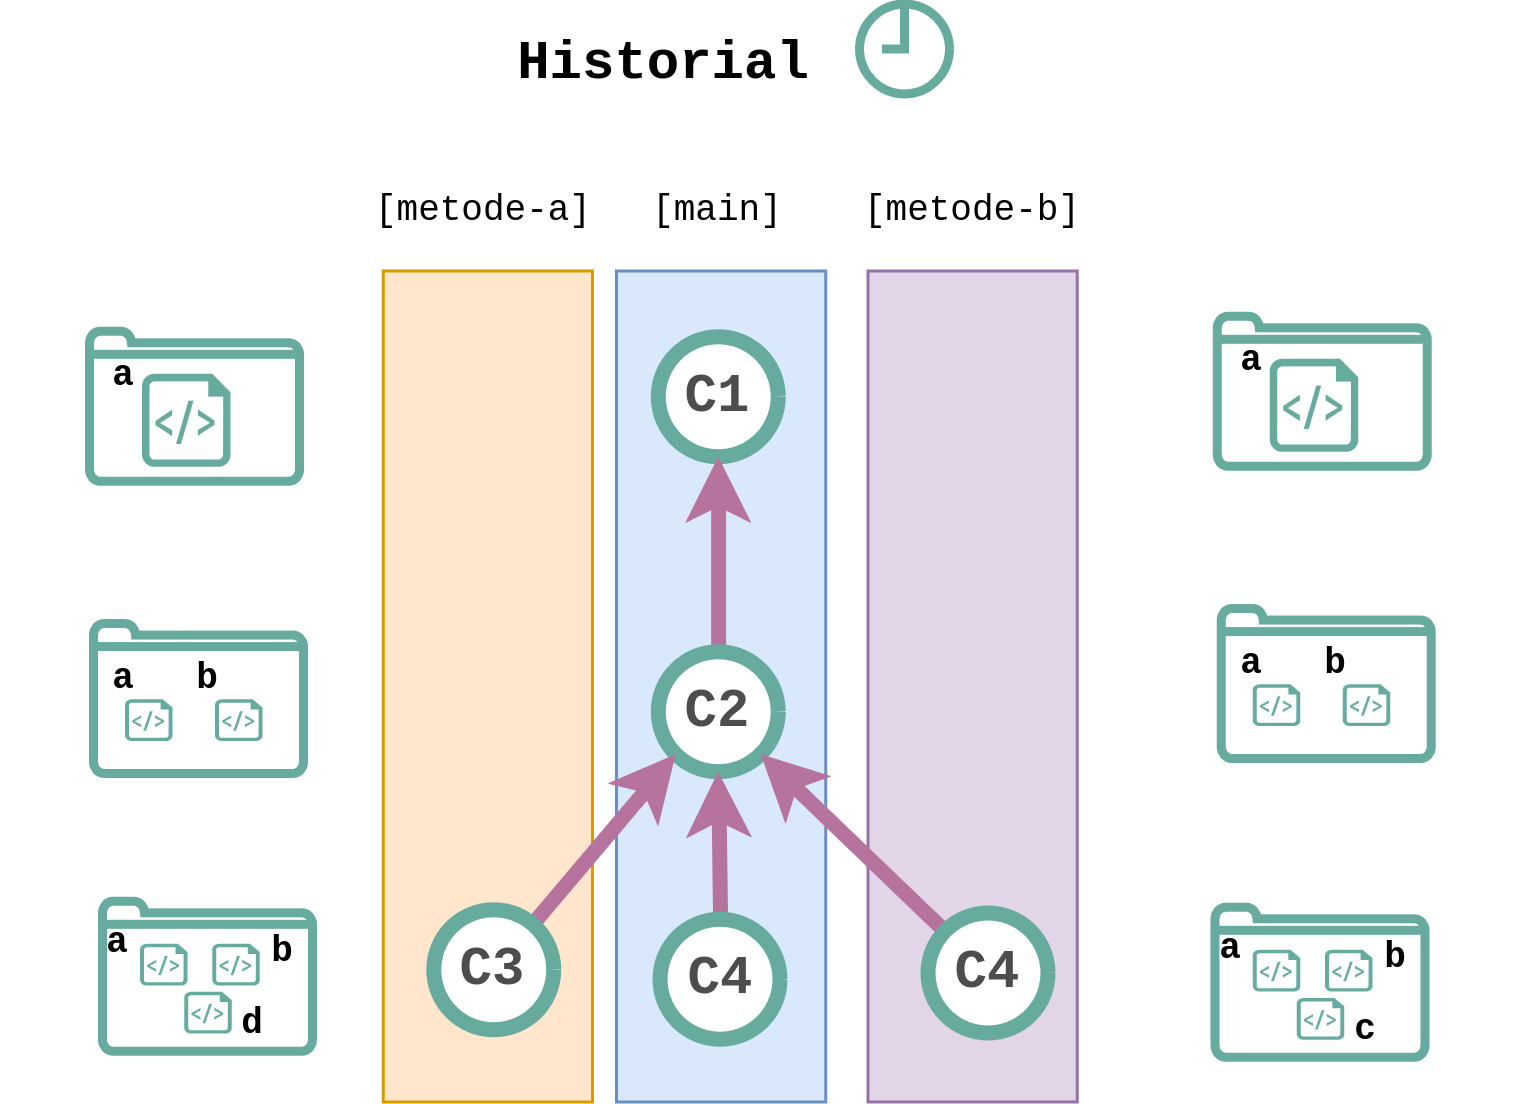
\includegraphics[scale=0.15]{images/merge}}
        \end{figure}
    \end{frame}
    \begin{frame}
        \frametitle{Merge and rebase}
        \begin{itemize}
            \item \texttt{git merge <branch>}: Merge the specified branch into the current branch
            \item \texttt{git rebase <branch>}: Rebase the current branch onto the specified branch
        \end{itemize}
    \end{frame}
    \begin{frame}
        \frametitle{Merge and rebase}
        \begin{figure}[H]
            \centering
            \noindent
            \makebox[\textwidth]{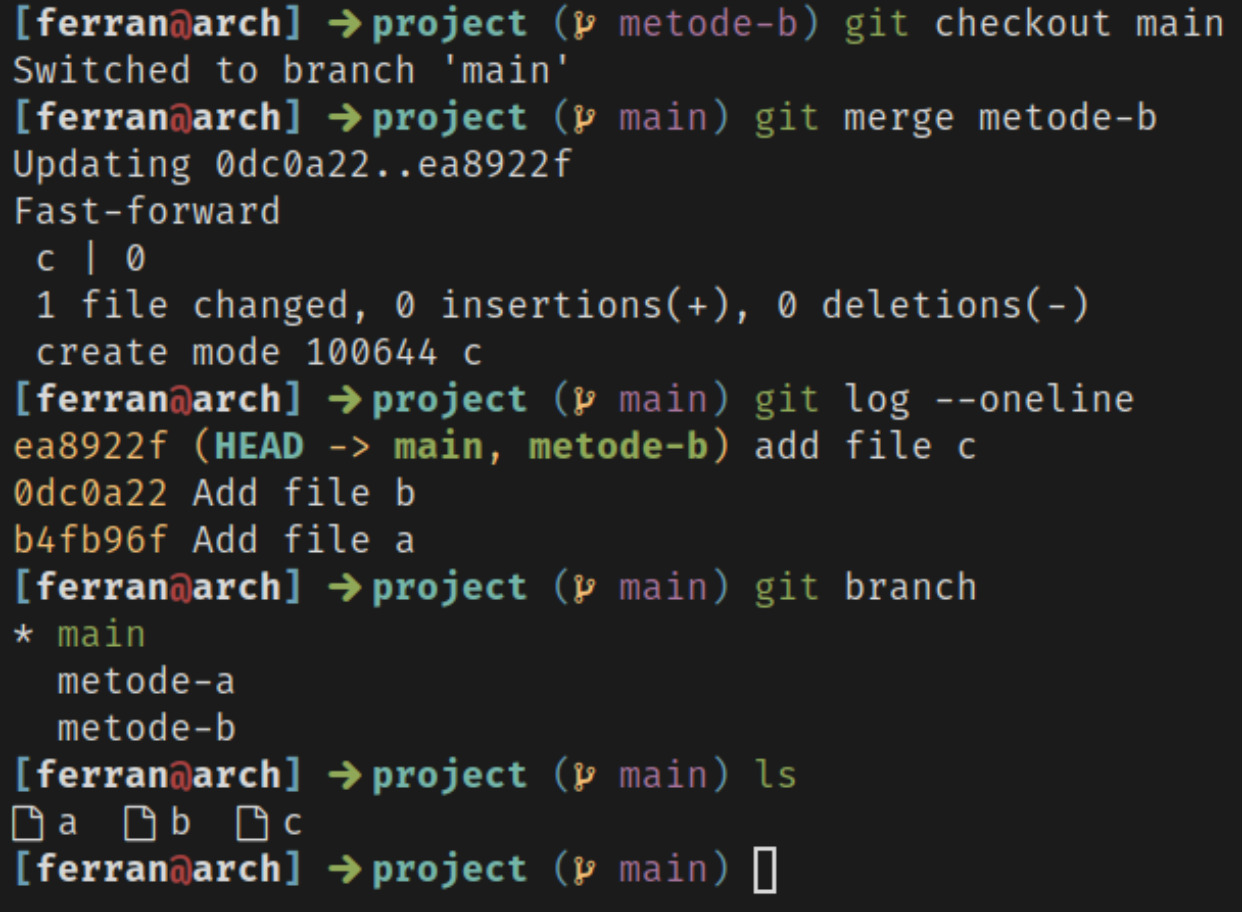
\includegraphics[scale=0.15]{images/merge-com-1}}
        \end{figure}
    \end{frame}
    \begin{frame}
        \frametitle{Merge and rebase}
        \begin{figure}[H]
            \centering
            \noindent
            \makebox[\textwidth]{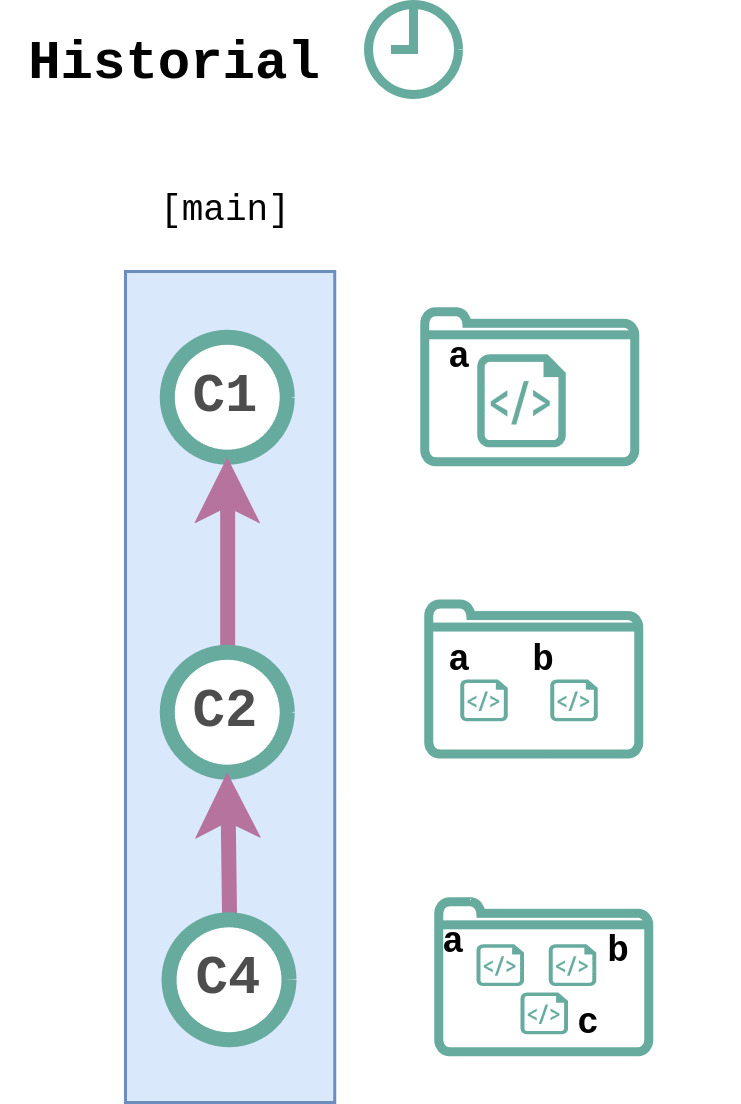
\includegraphics[scale=0.15]{images/merge-2}}
        \end{figure}
    \end{frame}
    \begin{frame}
        \frametitle{Merge and rebase}
        \begin{figure}[H]
            \centering
            \noindent
            \makebox[\textwidth]{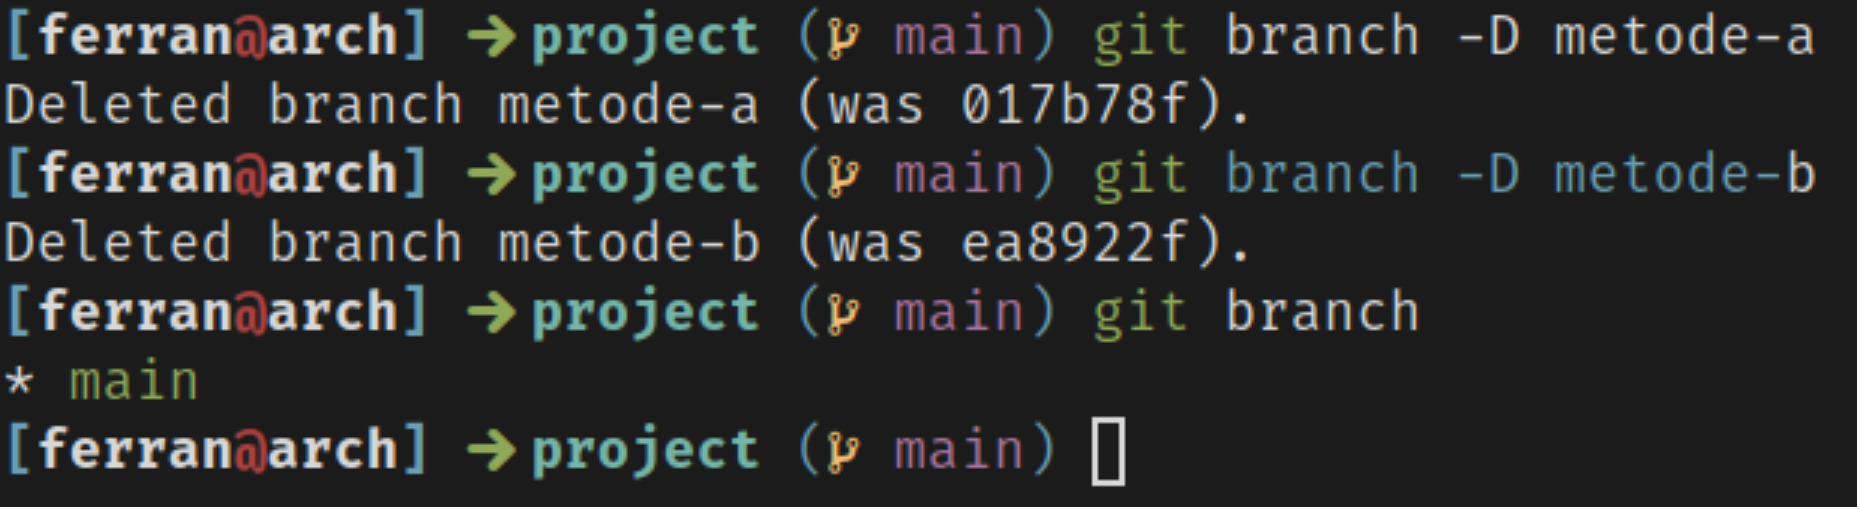
\includegraphics[scale=0.15]{images/merge-com-2}}
        \end{figure}
    \end{frame}

    \subsection{Standard commits}\label{subsec:standard-commits}
    \begin{frame}
        \frametitle{Standard commits}
        Standard commits are a set of rules to write commit messages that makes them more readable and easier to understand.
        They are based on the following structure:
        \begin{itemize}
            \item \texttt{<type>(<scope>): <subject>}
            \item \texttt{<body>}
            \item \texttt{<footer>}
        \end{itemize}
        The different types are:
        \begin{itemize}
            \item \texttt{feat}: A new feature
            \item \texttt{fix}: A bug fix
            \item \texttt{docs}: Documentation changes
            \item \texttt{refactor}: A code change that neither fixes a bug nor adds a feature
            \item \texttt{ci}: Changes to the CI configuration files and scripts
            \item \texttt{test}: Adding missing tests
        \end{itemize}
    \end{frame}
    \begin{frame}
        \frametitle{Standard commits}
        \begin{figure}[H]
            \centering
            \noindent
            \makebox[\textwidth]{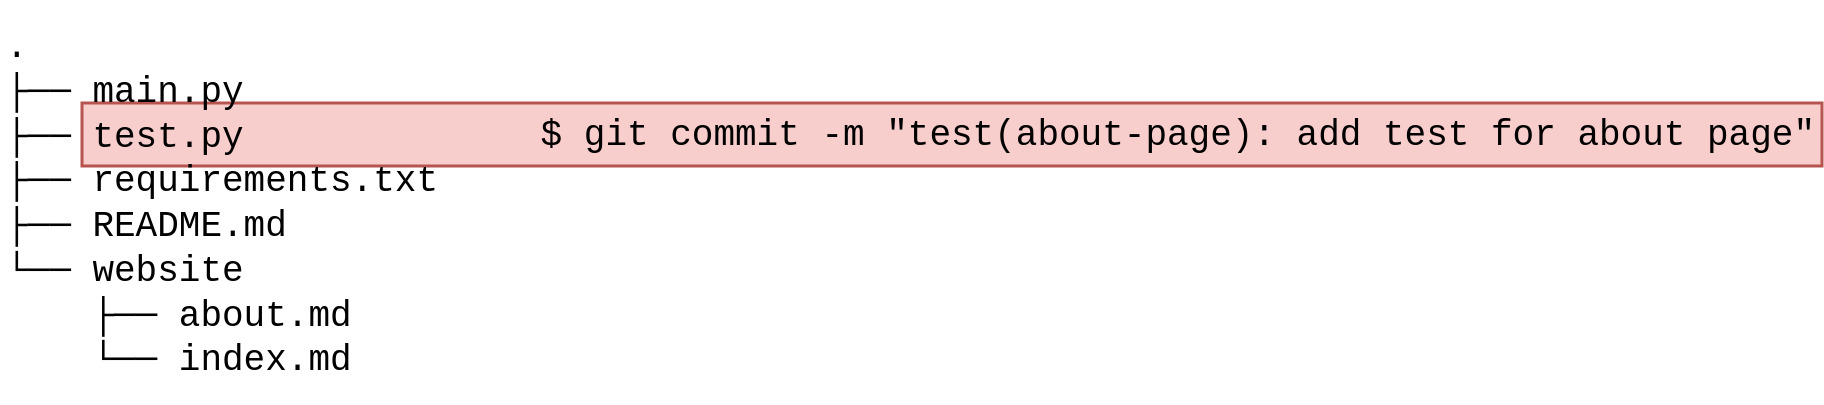
\includegraphics[scale=0.15]{images/st1}}
        \end{figure}
    \end{frame}
    \begin{frame}
        \frametitle{Standard commits}
        \begin{figure}[H]
            \centering
            \noindent
            \makebox[\textwidth]{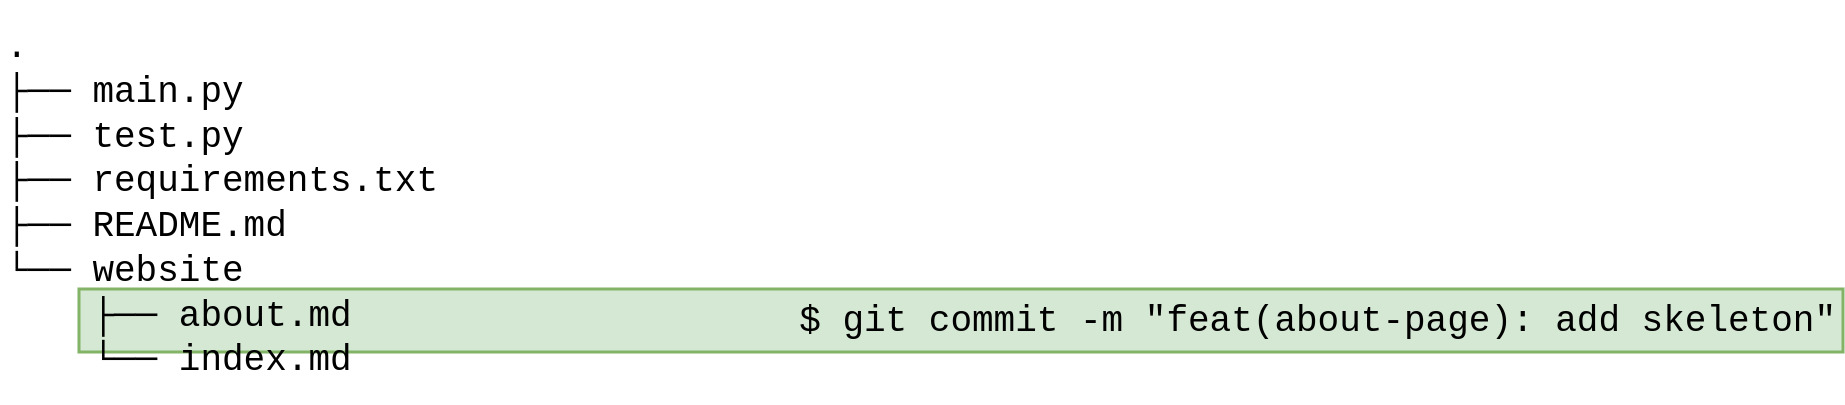
\includegraphics[scale=0.15]{images/st2}}
        \end{figure}
    \end{frame}
    \begin{frame}
        \frametitle{Standard commits}
        \begin{figure}[H]
            \centering
            \noindent
            \makebox[\textwidth]{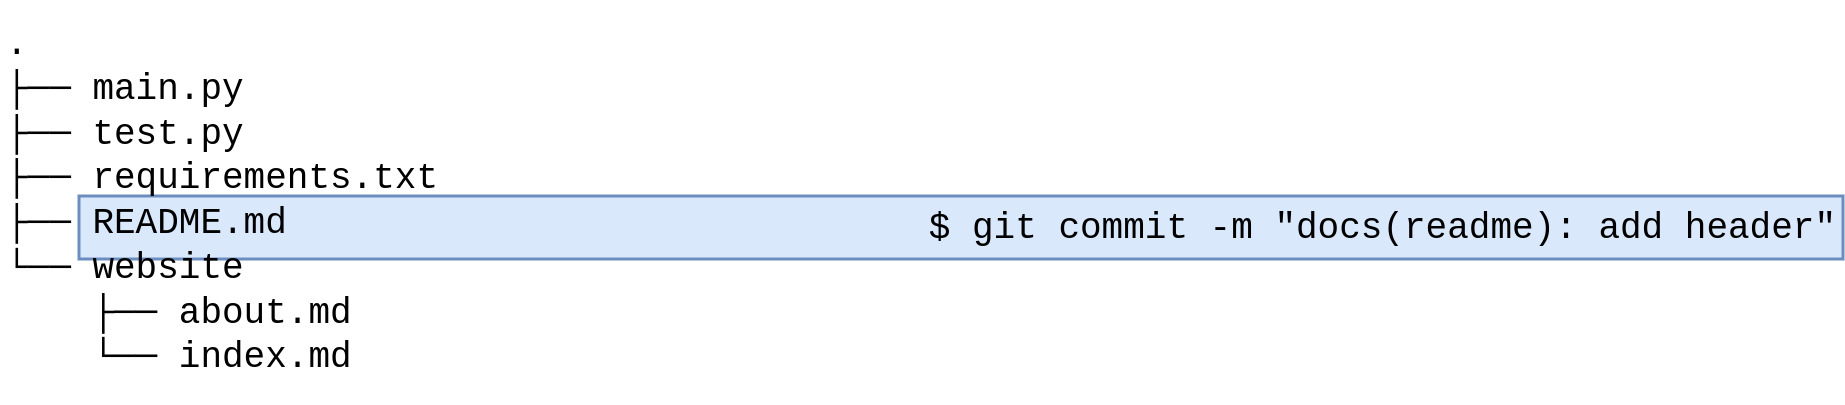
\includegraphics[scale=0.15]{images/st3}}
        \end{figure}
    \end{frame}
    \begin{frame}
        \frametitle{Standard commits}
        \begin{figure}[H]
            \centering
            \noindent
            \makebox[\textwidth]{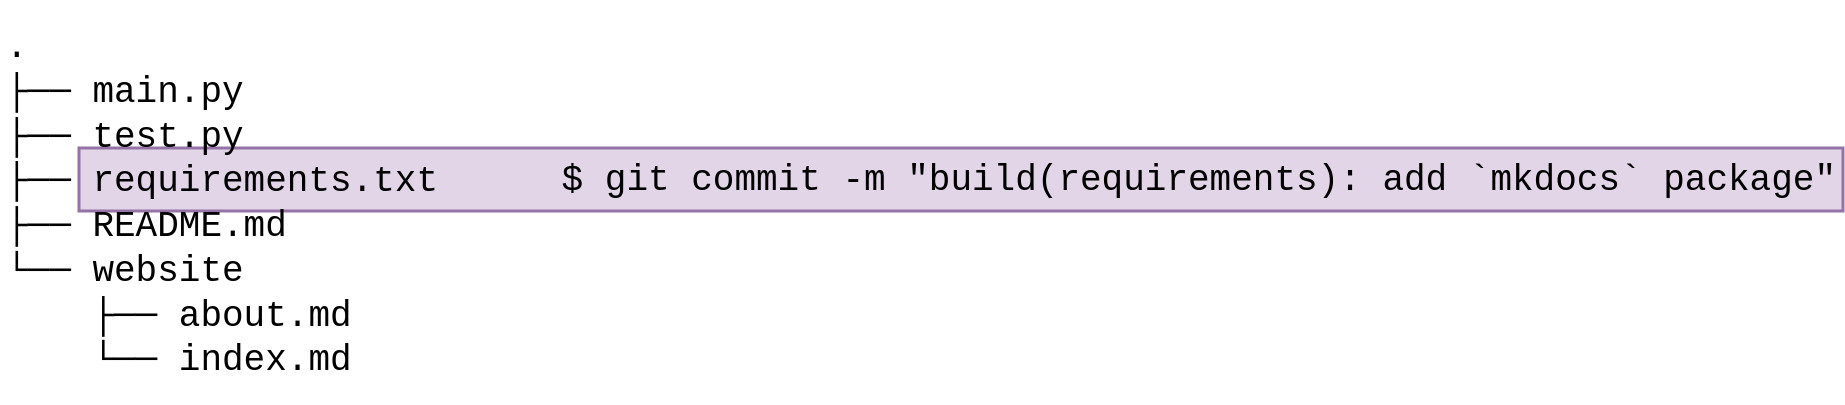
\includegraphics[scale=0.15]{images/st4}}
        \end{figure}
    \end{frame}
    \begin{frame}
        \frametitle{Standard commits}
        \begin{figure}[H]
            \centering
            \noindent
            \makebox[\textwidth]{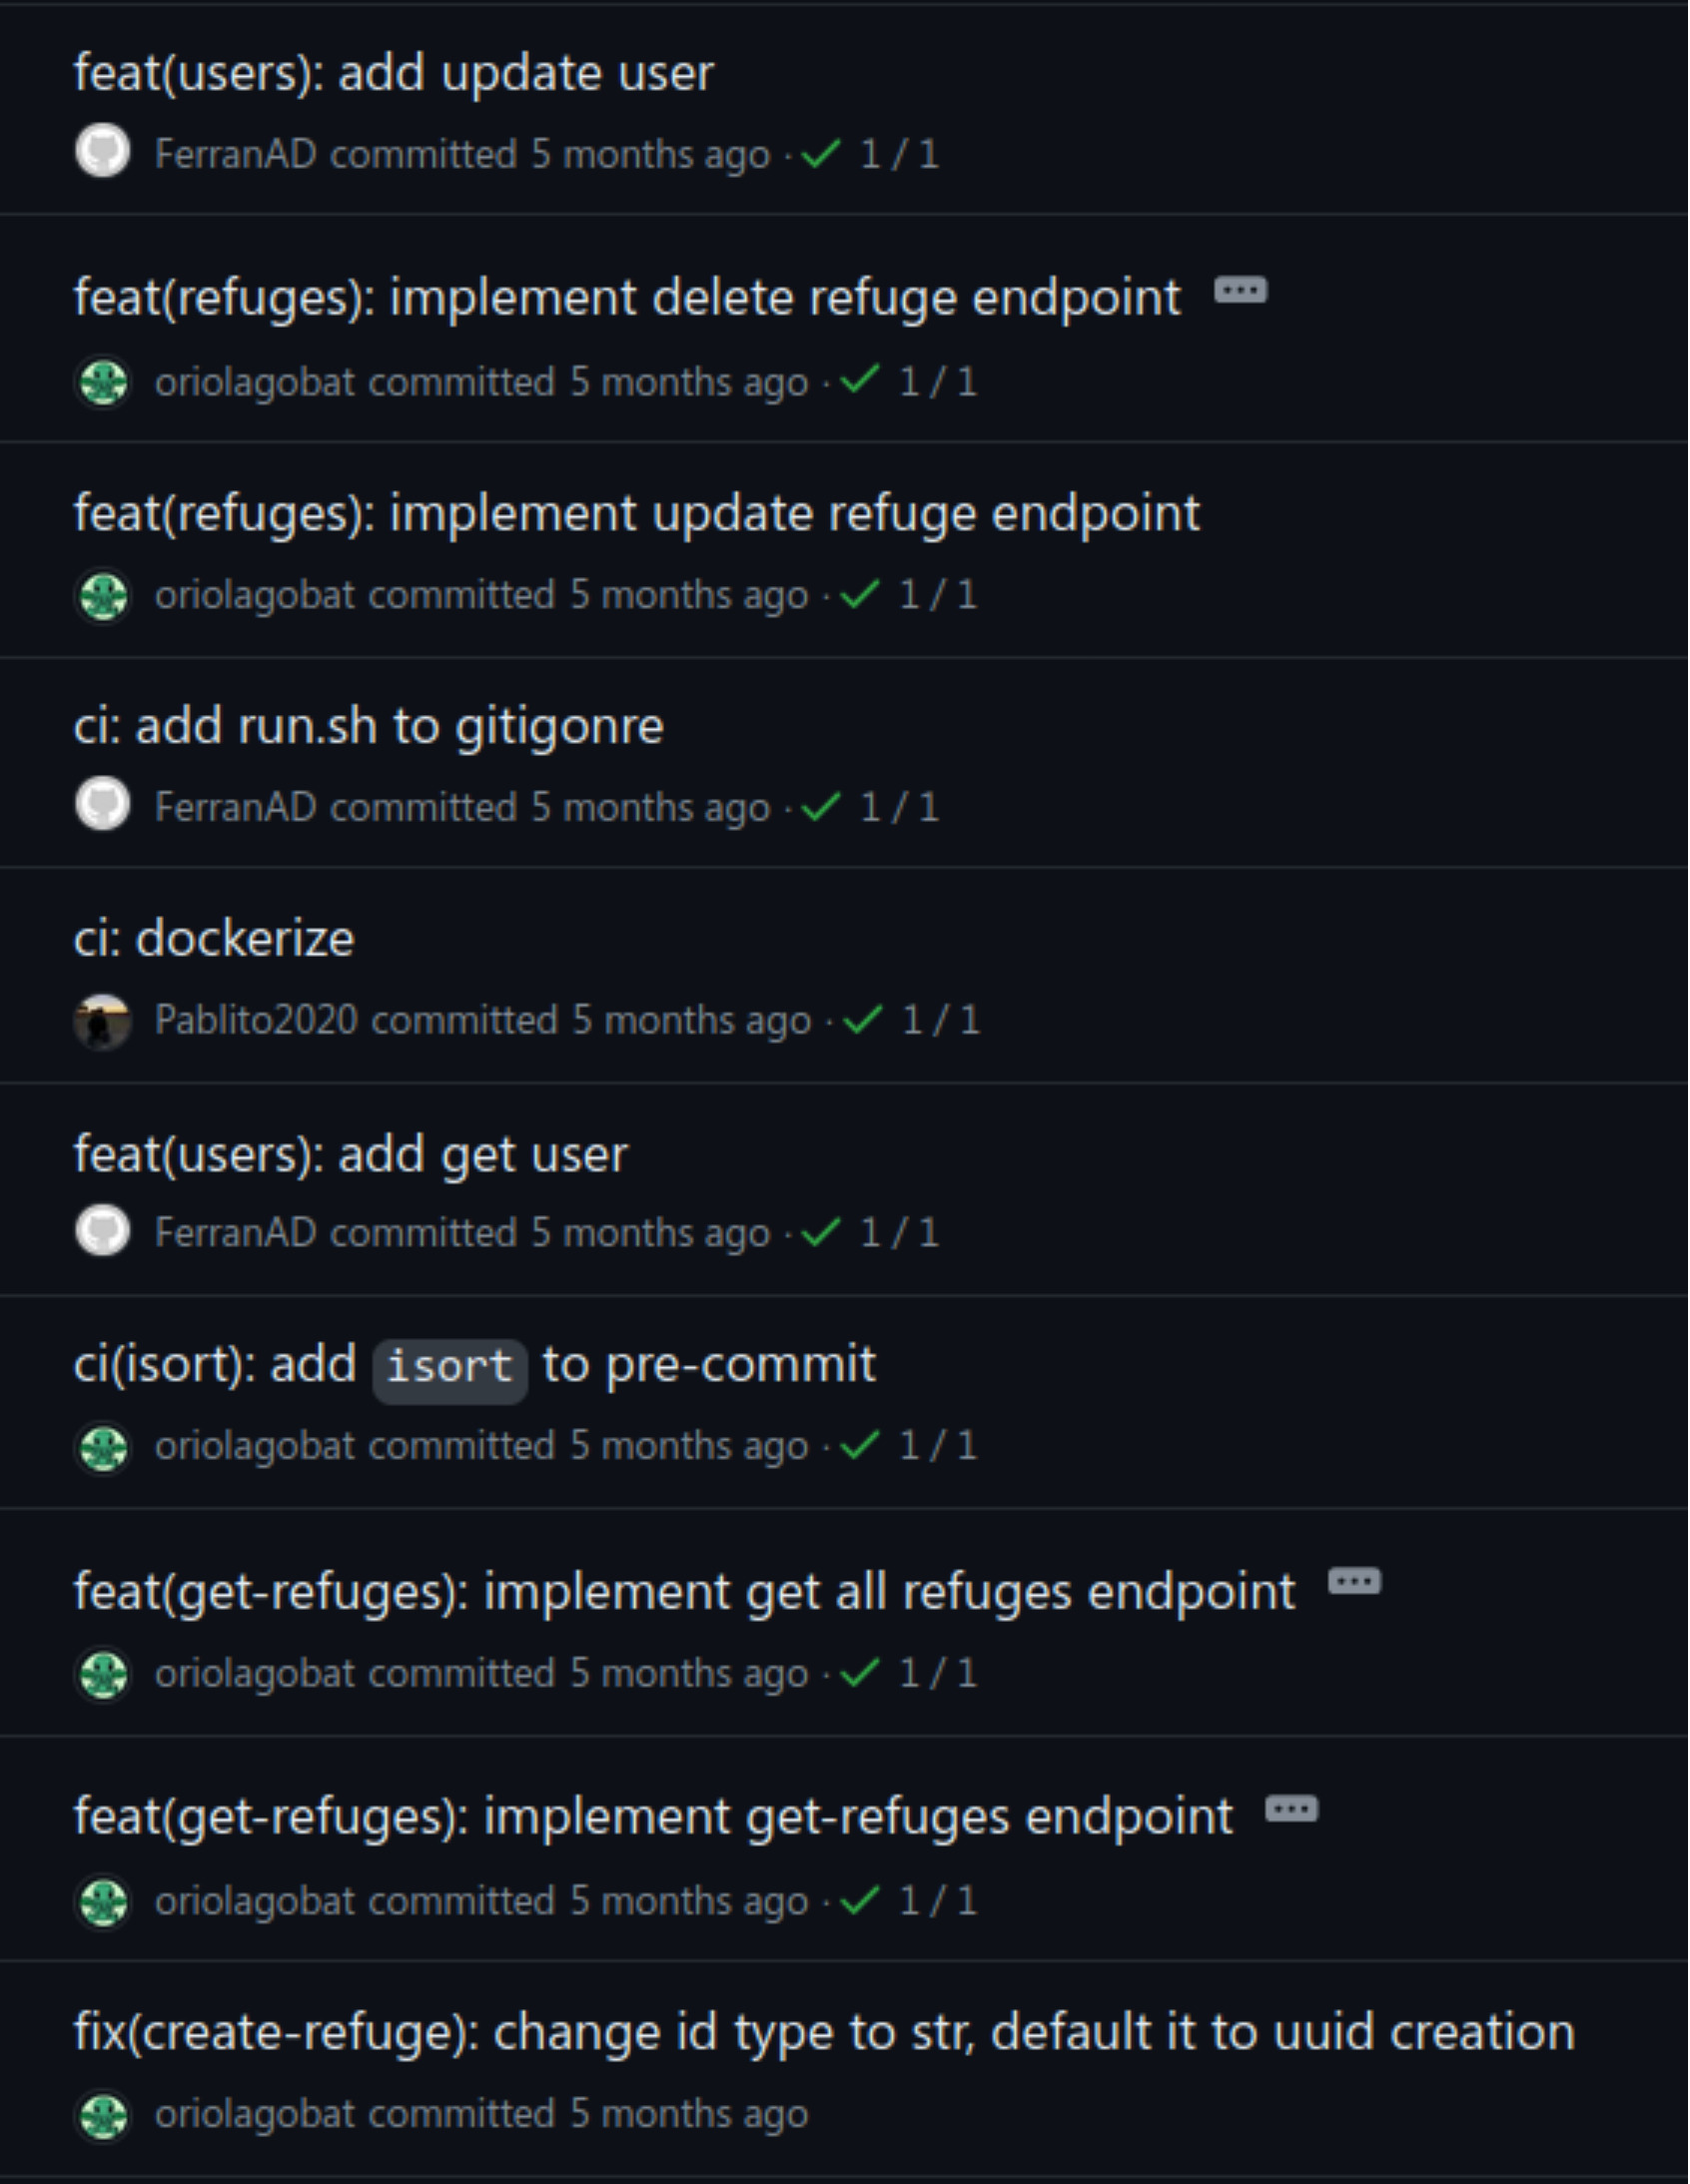
\includegraphics[scale=0.08]{images/st5}}
        \end{figure}
    \end{frame}
    \begin{frame}
        \frametitle{Standard commits}
        \begin{itemize}
            \item \url{https://github.com/RefuAPP/refuapp}
            \item \url{https://github.com/Spam-Number-Filter/Spam-Filter-WebPage}
            \item \url{https://github.com/SNMP-Python/snmp-data-analyzer}
            \item \url{https://github.com/ToDoTurtle/ToDoTurtle-Android}
            \item \url{https://github.com/hackudc-unplug/backend}
        \end{itemize}
    \end{frame}

    \subsection{Merge vs Rebase}\label{subsec:merge-rebase}
    \begin{frame}
        \frametitle{Merge vs Rebase}
        \begin{itemize}
            \item \textbf{Merge:}
                \begin{itemize}
                    \item Integrates changes from another branch into the current branch.
                    \item Creates a new commit with a merge message.
                    \item Maintains a linear history with clear separation of work.
                \end{itemize}
            \item \textbf{Rebase:}
                \begin{itemize}
                    \item Replays your commits on top of another branch.
                    \item Rewrites history, making the current branch appear as if the commits were originally made on the other branch.
                    \item Creates a cleaner linear history but can be risky if the branch has already been shared.
                \end{itemize}
        \end{itemize}
    \end{frame}

    \begin{frame}
        \frametitle{Merge vs Rebase}
        \item \textbf{Use Merge:}
        \begin{itemize}
            \item When collaborating with others and want a clear history of who made what changes.
            \item When the branch being merged into has already been shared with others.
        \end{itemize}
    
        \textbf{Use Rebase:}
        \begin{itemize}
            \item When working on a private branch and want a clean, linear history.
            \item Before pushing your branch to a shared repository to avoid merge commits.
        \end{itemize}
    \end{frame}

    \begin{frame}
       \begin{itemize}
           \item {\textbf{\texttt{git merge <branch-name>}}}: Merges the specified branch into the current branch.
           \item {\textbf{\texttt{git rebase <branch-name>}}}: Rebases the current branch onto the specified branch.
           \item {\textbf{\texttt{git merge --abort}}}: Aborts a merge that is in progress.
           \item {\textbf{\texttt{git rebase --abort}}}: Aborts a rebase that is in progress.
       \end{itemize}
   \end{frame}

    \subsection{Gitignore}\label{subsec:gitignore}
    \begin{frame}
        \frametitle{Gitignore}
        \begin{figure}[H]
            \centering
            \noindent
            \makebox[\textwidth]{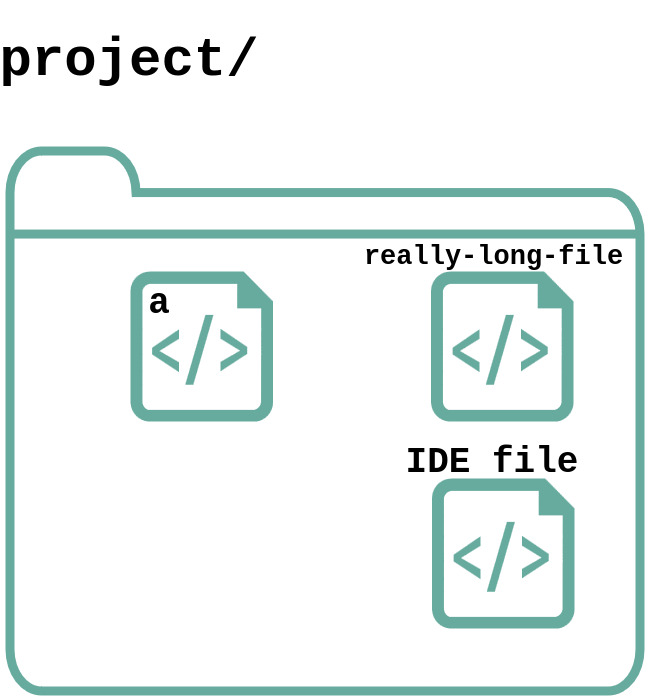
\includegraphics[scale=0.15]{images/gi1}}
        \end{figure}
    \end{frame}
    \begin{frame}
        \frametitle{Gitignore}
        \begin{figure}[H]
            \centering
            \noindent
            \makebox[\textwidth]{
\includegraphics[scale=0.1]{images/gi2}}
        \end{figure}
    \end{frame}
    \begin{frame}
        \frametitle{Gitignore}
        \begin{figure}[H]
            \centering
            \noindent
            \makebox[\textwidth]{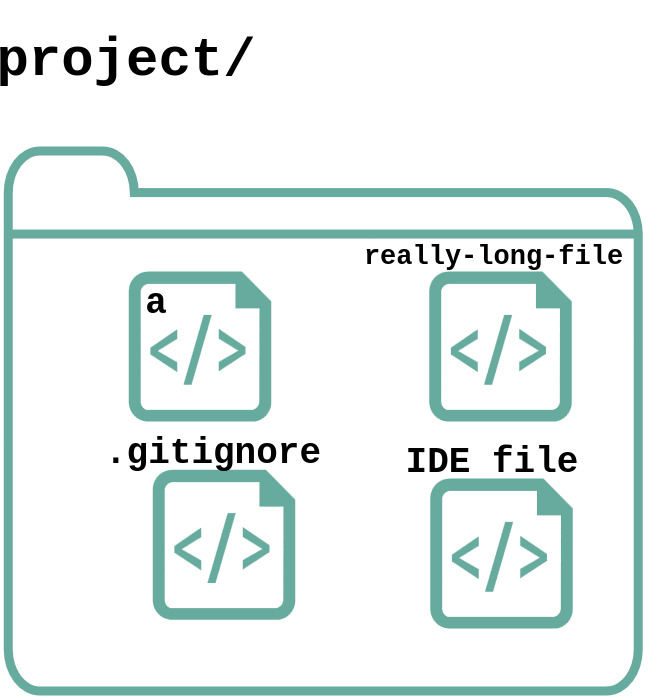
\includegraphics[scale=0.15]{images/gi3}}
        \end{figure}
    \end{frame}
    \begin{frame}
        \frametitle{Gitignore}
        \begin{figure}[H]
            \centering
            \noindent
            \makebox[\textwidth]{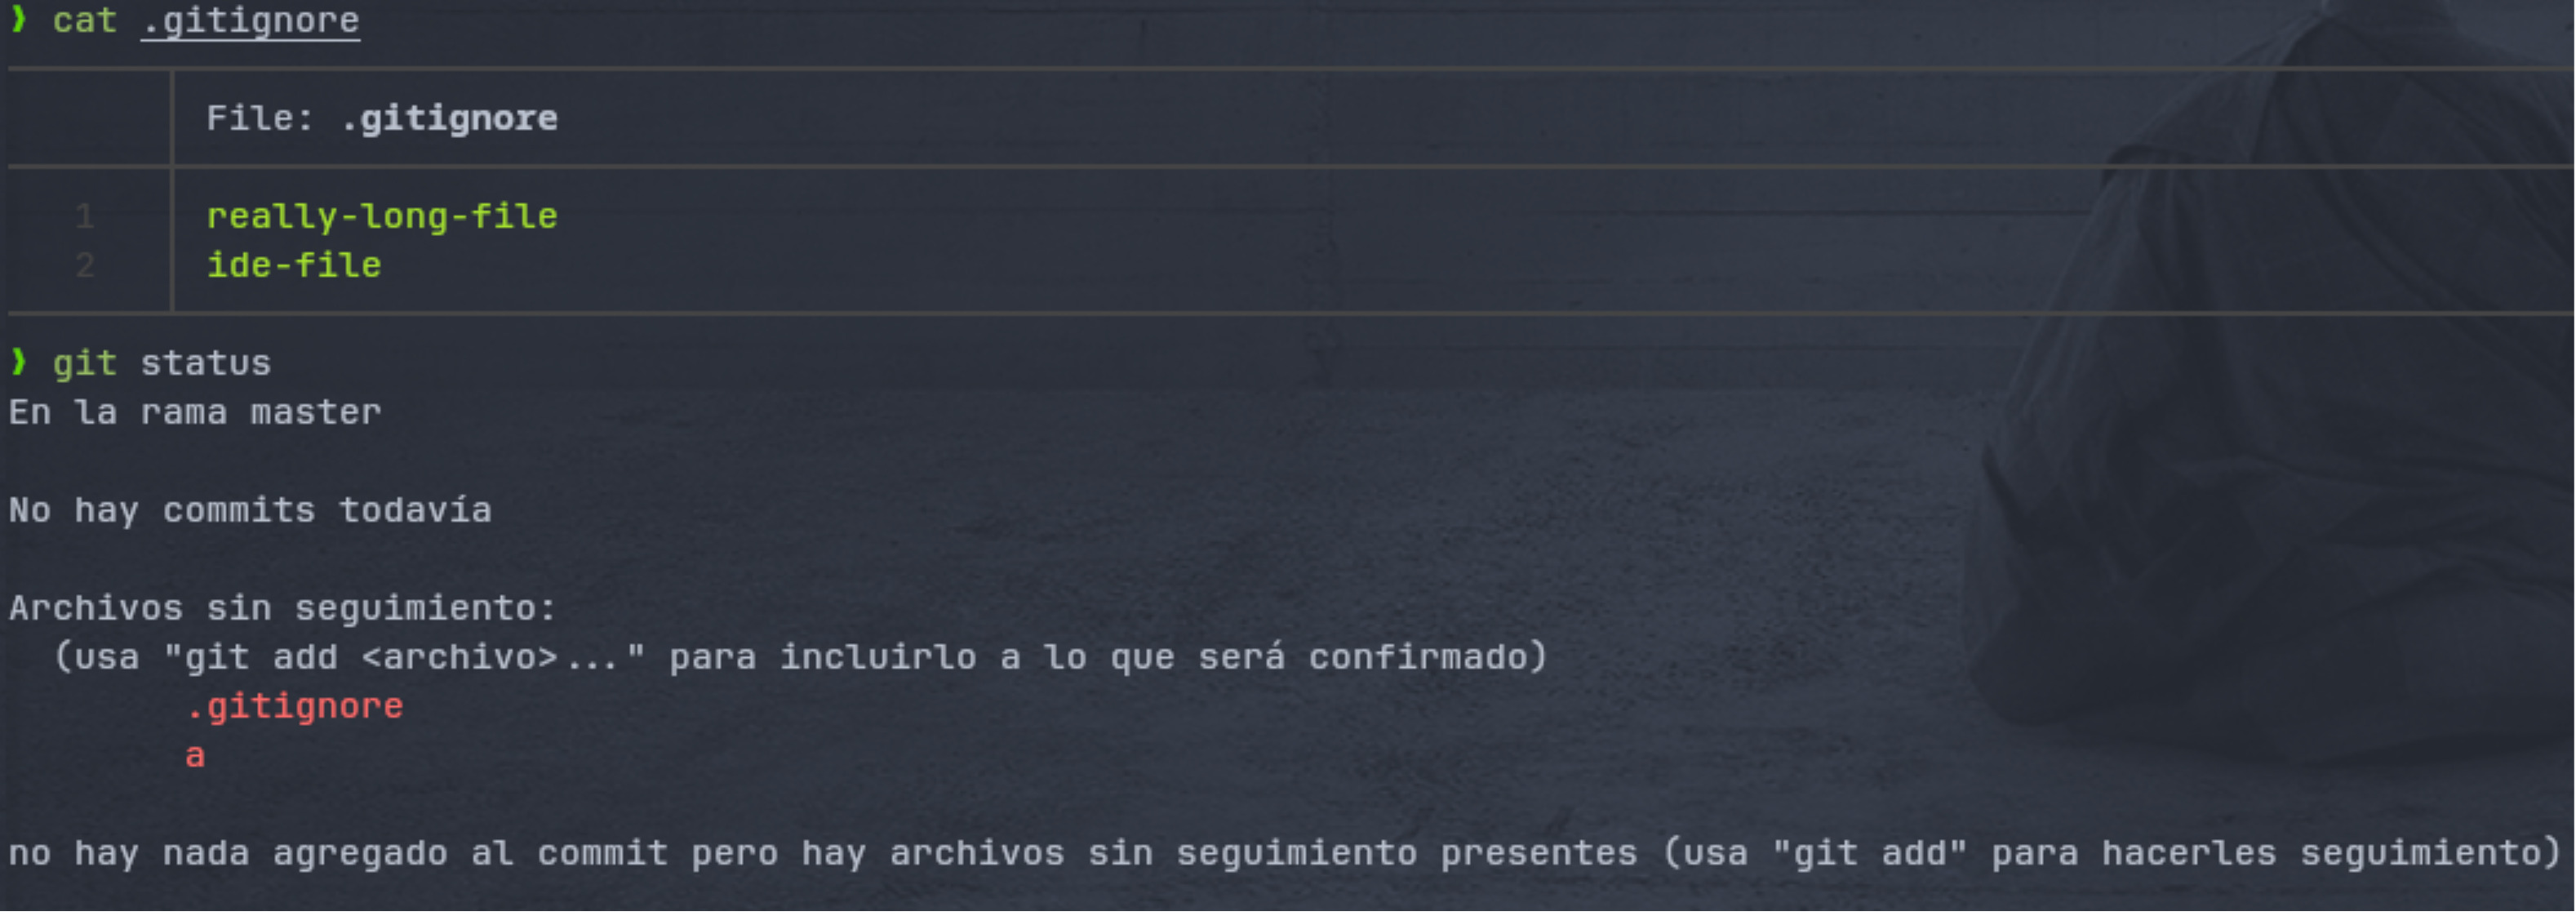
\includegraphics[scale=0.1]{images/gi4}}
        \end{figure}
    \end{frame}
    \begin{frame}
        \frametitle{Gitignore}
        \begin{figure}[H]
            \centering
            \noindent
            \makebox[\textwidth]{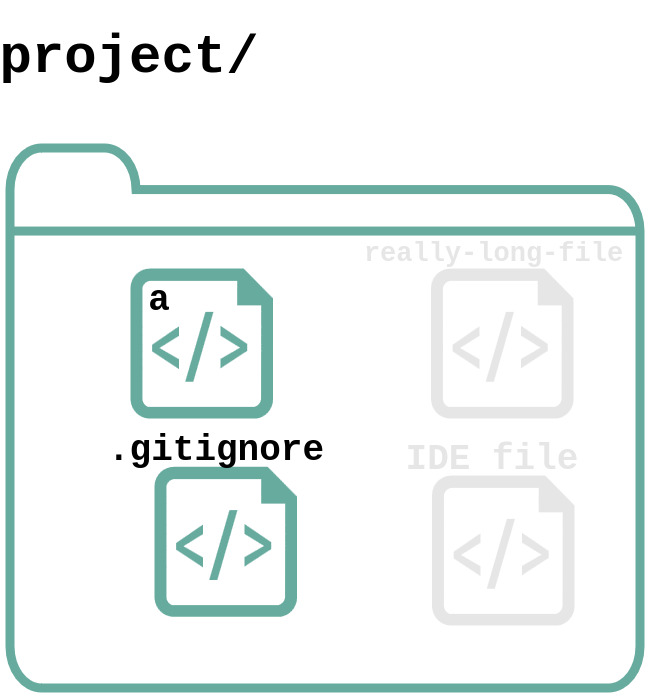
\includegraphics[scale=0.15]{images/gi5}}
        \end{figure}
    \end{frame}

    \subsection{Stash}\label{subsec:stash}
    \begin{frame}
        \frametitle{Stash}
        Git stash allows you to temporarily save your uncommitted changes without losing them. This is useful when you need to switch tasks or want to keep your working directory clean.
    \end{frame}

    \begin{frame}
        \begin{itemize}
            \item \texttt{git stash}: Creates a stash entry, saving your uncommitted changes.
            \item \texttt{git stash list}: Shows a list of all your stashed changes.
            \item \texttt{git stash apply <stash@{n}>}: Applies the most recent stash (or the nth stash) on top of your current work.
            \item \texttt{git stash pop <stash@{n}>}: Applies the most recent stash (or the nth stash) and removes it from the stash list.
            \item \texttt{git stash drop <stash@{n}>}: Removes the specified stash entry from the list.
        \end{itemize}
    \end{frame}

    \subsection{Coauthor}\label{subsec:coauthor}
    \begin{frame}
        \frametitle{Coauthor}
        In Git, commits are attributed to the user who committed them by default. However, you can add co-authors to a past commit if someone else contributed to the changes.

        \textbf{Important note}: Modifying past commits directly is generally discouraged as it rewrites history and can cause issues in shared repositories. Use this feature with caution.
    \end{frame}

    \begin{frame}
        There are two main approaches to adding a co-author:

        1. \textbf{Interactive rebase:}
            \begin{itemize}
                \item Use \texttt{git rebase -i <commit-hash>} to initiate interactive rebase.
                \item Edit the commit message and add the co-author using the format: "Co-authored-by: Name <email>".
                \item Save and continue the rebase to apply the changes.
            \end{itemize}

        2. \textbf{Commit amend:}
            \begin{itemize}
                \item Use \texttt{git commit --amend} to open the commit message editor for the latest commit.
                \item Add the co-author line in the format: "Co-authored-by: Name <email>".
                \item Stage any additional changes and save the commit message.
            \end{itemize}
    \end{frame}

    \subsection{Rebase interactive}\label{subsec:rebase-interactive}

    \begin{frame}
        \frametitle{Rebase Interactive}
        Git rebase interactive allows you to rewrite commit history by modifying or discarding commits. This can be helpful for cleaning up your branch history, squashing multiple commits into one, or fixing mistakes.

        \textbf{Use with caution:} Rebasing rewrites history, so ensure the branch hasn't been shared with others before using this feature.
    \end{frame}

    \begin{frame}
        Steps to perform an interactive rebase:

        1. Run \texttt{git rebase -i <starting-commit-hash>}. This opens an editor showing your commit history.
        2. Edit the instruction next to each commit:
            \begin{itemize}
                \item pick: Keep the commit unchanged.
                \item edit: Modify the commit message and content.
                \item squash: Combine the current commit with the previous one.
                \item drop: Discard the commit.
            \end{itemize}
        3. Save the changes in the editor.
        4. Git will replay the commits based on your instructions, rewriting the branch history.
    \end{frame}

    \subsection{Reflog}\label{subsec:reflog}
    \begin{frame}
        \frametitle{Reflog}
        The reflog is a log of all HEAD (reference) movements in your Git repository. It tracks every time the HEAD pointer changes, including commits, renames, merges, and reverts.

        This can be helpful for:
        \begin{itemize}
            \item Undoing accidental HEAD movements.
            \item Verifying the history of your commits.
            \item Recovering from lost commits.
        \end{itemize}
    \end{frame>

    \begin{frame}
        \frametitle{Viewing the Reflog}


        There are two main ways to view the reflog:\\

        1. \textbf{`git reflog show`:} This command displays the complete reflog by default. You can also use the `-n` flag to specify the number of entries to show.

        ```
        git reflog show
        git reflog show -n 10  # Show the last 10 entries
        ```

        2. \textbf{Filtering the Reflog:} You can filter the reflog output by providing a commit hash or a reference name.

        ```
        git reflog show <commit-hash>  # Show entries related to a specific commit
        git reflog show HEAD@{1.week.ago} # Show entries from a week ago
        ```
    \end{frame}
\end{document}